\documentclass[11pt]{article}
\usepackage[T1]{fontenc}
\usepackage[utf8]{inputenc}
\usepackage{lmodern}
\usepackage[margin=2.3cm]{geometry}
\usepackage{booktabs,longtable,array,graphicx,amsmath,url,hyperref,float,caption,enumitem,xcolor}
\usepackage{listings}
\usepackage{fancyhdr}
\usepackage{titlesec}
\usepackage{microtype}
\usepackage{placeins}
\usepackage{textcomp}

\renewcommand{\arraystretch}{1.12}
\newcolumntype{L}[1]{>{\raggedright\arraybackslash}p{#1}}
\graphicspath{{figures/}{../../final_work_deliverable_2/figures/}{../../outputs/eda_charts/}}
\hypersetup{colorlinks=true,linkcolor=blue,urlcolor=blue,citecolor=blue}
\captionsetup{font=small,labelfont=bf}

% Header and footer
\pagestyle{fancy}
\fancyhf{}
\fancyhead[L]{\small SmogShield Lahore --- Final Report}
\fancyhead[R]{\small\thepage}
\renewcommand{\headrulewidth}{0.4pt}

% Code listings
\lstset{
  basicstyle=\ttfamily\small,
  breaklines=true,
  frame=single,
  columns=fullflexible,
  keepspaces=true,
  showstringspaces=false
}

\title{\textbf{SmogShield Lahore}\\[3mm]
Final Report: Deliverables 1--3, Phases 1--6\\[2mm]
\large Problem Definition, Data Foundations, Modelling, Evaluation,\\
\large and the Deliverable 3 Application and Explainability Layer}
\author{Muhammad Haider Mughal (3006) \and Muhammad Ayub Butt (3076) \and Abdul Rehman (3059)}
\date{12 November 2026}

\begin{document}
\maketitle
\thispagestyle{empty}

\begin{abstract}
\noindent
SmogShield is an explainable next-day air-quality forecasting system for
Lahore. This report integrates the three deliverables and the six project
phases: the problem definition, the data foundations, the frozen modelling
core, the evaluation and bias analysis, the Deliverable 3 application, and the
final evaluation. The data cover 2,113 daily rows from 23 May 2019 to 4 March
2025, built from one OpenAQ PM$_{2.5}$ monitor, daily weather, and calendar
features. The modelling core is a histogram gradient-boosting regressor for
next-day PM$_{2.5}$ and a six-class histogram gradient-boosting classifier for
next-day AQI category, selected on a chronological validation split with a
seven-day purge. On the held-out test split, the regression essentially ties
persistence (RMSE 64.92 versus 64.82 $\mu$g/m$^3$; skill $-0.0016$) and the
classifier is weaker than persistence on macro-F1 (0.478 versus 0.516). These
results are reported without retuning on test. Deliverable 3 adds a Streamlit
application with six user inputs, two category views, an 80\% prediction
interval (80.3\% validation coverage, 77.0\% test coverage), local sensitivity
and global permutation importance, historical seasonal and hourly context, and
a persistence comparison on every forecast. The application has 14 passing
tests and a render smoke test. The project's contribution is an honest,
reproducible, explainable end-to-end system, not a claim of beating a strong
one-day baseline.
\end{abstract}

\vspace{2mm}
\begin{table}[htbp]
\centering
\small
\renewcommand{\arraystretch}{1.25}
\begin{tabular}{@{}L{6.6cm}L{7.4cm}@{}}
\toprule
\textbf{Question} & \textbf{Answer in this report} \\
\midrule
Does the regression beat persistence? &
No. Test RMSE 64.92 versus 64.82 $\mu$g/m$^3$; skill $-0.0016$. \\
Does the classifier beat persistence? &
No. Test macro-F1 0.478 versus 0.516. \\
What is new in Deliverable 3? &
The application, inference, 80\% intervals, explanations, seasonal context,
hourly profile, ablation, tests, and report. \\
What does the app forecast? &
Tomorrow's PM$_{2.5}$ and AQI category from six values for today. \\
What is the honest verdict? &
A reproducible, explainable demonstrator; not an operational warning system. \\
\bottomrule
\end{tabular}
\caption{Key results at a glance.}
\label{tab:glance}
\end{table}

\newpage
\tableofcontents
\newpage

% Phase 1: Problem Definition (included by report_main_final.tex).
% Needs in the main file's preamble: \usepackage{array,booktabs,enumitem}
% and this line:  \newcolumntype{L}[1]{>{\raggedright\arraybackslash}p{#1}}
% Citations resolve against the thebibliography block in report_main_final.tex.

\section{Phase 1: Problem Definition}

\subsection{Problem Statement}

Lahore experiences recurring episodes of severe air pollution, most visibly during the winter ``smog season'' that roughly spans October to February~\cite{majeed2024lahore}. The pollutant most often used to describe these episodes is fine particulate matter (PM$_{2.5}$), particles smaller than 2.5~$\mu$m that can be inhaled deeply~\cite{who2024ambient,epa_pm_basics}.

Our own data shows how persistent the problem is. The US Diplomatic Post monitor in Lahore recorded at least 18 valid hourly readings on 1{,}506 days between May 2019 and March 2025. Converting each day's mean PM$_{2.5}$ to the US EPA Air Quality Index (AQI, 2012 breakpoints)~\cite{epa_aqi_tad}, only 9 of those days (0.6\%) fell in the ``Good'' category, while 1{,}102 days (73.2\%) were ``Unhealthy'' or worse. These figures come from a single monitor and from days with enough valid readings, so they describe the data we have rather than the whole city.

\paragraph{The pain point.} A resident deciding whether to cycle to work, hold a school sports session, or work outdoors tomorrow needs three things: a forecast, an idea of how reliable it is, and a reason for it. Air-quality information is commonly presented as a current reading, which leaves three gaps:
\begin{itemize}
  \item \textbf{Timing:} a current value does not say what tomorrow will look like.
  \item \textbf{Trust:} a single number gives no sense of how uncertain it is.
  \item \textbf{Understanding:} people are rarely told which conditions (for example calm air, cold temperatures, high humidity) are driving the pollution.
\end{itemize}

\paragraph{Our solution.} SmogShield Lahore is a web application that forecasts the next day's PM$_{2.5}$ level and AQI category for Lahore from historical air-quality and weather data (with calendar-based proxies where traffic data is unavailable). Each forecast comes with a prediction interval, the main factors the model relied on, and cautious, non-medical guidance. The project also studies recurring seasonal pollution patterns and tests whether adding weather and calendar information improves forecast accuracy.

\subsection{Target Audience}

\begin{table}[h]
\centering
\small
\begin{tabular}{L{3.6cm}L{4.6cm}L{5.6cm}}
\toprule
\textbf{User group} & \textbf{Decision they face} & \textbf{What SmogShield provides} \\
\midrule
Commuters, cyclists and runners & Whether to travel or exercise outdoors tomorrow & Next-day AQI category with an uncertainty range \\
Parents and schools & Whether to hold outdoor activities & Category-based, cautious guidance \\
Outdoor workers & Planning the working day & Forecast and typical cleaner hours from historical patterns \\
Residents who may be sensitive to air pollution, and their carers & Deciding how cautious to be & The forecast category and the factors behind it (not medical advice) \\
Students and researchers & Assessing a transparent baseline & Documented data, models and limitations \\
\bottomrule
\end{tabular}
\caption{Target users and how the application supports their decisions.}
\end{table}

The primary audience is the general public in Lahore. SmogShield is not a medical tool and does not replace official public-health advisories.

\subsection{AI Justification}

A rule-based system would encode expert thresholds such as ``if wind speed is below X and humidity is above Y, predict poor air quality.'' Machine-learning models have already been used to forecast Lahore's AQI from historical series~\cite{waqas2024lahore}; SmogShield extends this line by forecasting next-day PM$_{2.5}$ with weather and calendar inputs and by attaching uncertainty and explanations to each forecast. We argue that machine learning is better suited to this problem for the following reasons.

\begin{enumerate}
  \item \textbf{Many interacting factors.} Tomorrow's PM$_{2.5}$ depends on today's level and on wind speed and direction, humidity, dew point, temperature, pressure, rainfall and the time of year. The effect of one factor depends on the others (for example, calm air matters most when it is also cold and humid). Writing and justifying thresholds for every combination by hand does not scale, whereas learning algorithms such as tree ensembles fit these interactions directly from data.
  \item \textbf{Relationships change with the season.} The same wind speed does not mean the same thing in a monsoon July and in a December smog episode. Rules would need separate hand-tuned sets for each regime. A model trained on several years of data can learn these differences.
  \item \textbf{Uncertainty has to be estimated.} A fixed rule gives a single answer. Learned models allow prediction intervals to be estimated from historical forecast errors (for example with quantile regression), which supports the trust gap described above.
  \item \textbf{The data is suitable.} We have an observed daily PM$_{2.5}$ series with 1{,}506 usable days, together with more than 2{,}600 days of daily weather. This is a tabular supervised learning problem with enough rows for tree-based models and regularised linear models, and possibly a small recurrent network for comparison.
  \item \textbf{Maintainability.} When new data arrives, a model can be retrained and re-evaluated. A rule set must be re-tuned manually.
  \item \textbf{Complement to physical models.} Atmospheric models exist, but a modeled air-quality dataset we examined during Phase 2 read about half as high as the monitor on overlapping days and under-read smog peaks. A statistical model trained on local observations is a practical complement.
\end{enumerate}

\paragraph{An honest counterpoint.} Daily pollution is strongly persistent, so a simple baseline that predicts ``tomorrow equals today'' is hard to beat. For this reason we compare every learned model against that persistence baseline and against simple linear models. We claim a benefit from machine learning only where the evaluation shows one.

\begin{table}[h]
\centering
\small
\begin{tabular}{L{4.0cm}L{4.9cm}L{4.9cm}}
\toprule
\textbf{Aspect} & \textbf{Rule-based} & \textbf{Machine learning} \\
\midrule
Factor interactions & Hand-written, limited & Learned from data \\
Seasonal differences & Separate rule sets & Learned, can use season as input \\
Uncertainty & Not provided & Estimated from past errors \\
Updating & Manual re-tuning & Retrain on new data \\
Evidence of accuracy & Hard to measure fairly & Compared with baselines on held-out data \\
\bottomrule
\end{tabular}
\caption{Why a learned model is preferred over fixed rules for this problem.}
\end{table}

\subsection{Research Questions and Scope}

\begin{enumerate}
  \item[\textbf{RQ1}] Can machine learning models forecast next-day PM$_{2.5}$ and AQI category better than a persistence baseline?
  \item[\textbf{RQ2}] Does adding weather, and then calendar information, improve accuracy compared with air-quality history alone (ablation study)?
  \item[\textbf{RQ3}] Where do the models fail? We examine errors by season and on extreme-pollution days.
\end{enumerate}

\paragraph{Scope and limitations.} The forecast is for the next day at daily resolution, for Lahore, based mainly on one reference monitor. Traffic is represented by calendar proxies because no open, time-aligned Lahore traffic dataset was found. The data has gaps, and the evaluation uses a time-based split so that no future information leaks into training. The application gives cautious guidance and is not medical advice.

% References are listed in the thebibliography block of report_main_final.tex.

% Phase 2: Data Foundations (included by report_main_final.tex).
% Needs in the main file's preamble:
%   \usepackage{array,booktabs,enumitem,graphicx,url,amsmath}
%   \newcolumntype{L}[1]{>{\raggedright\arraybackslash}p{#1}}
%   \graphicspath{{processed/eda_charts/}}

\section{Phase 2: Data Foundations}

Phase 2 turns the problem definition into a documented, reproducible dataset. This section records where every file came from, what was cleaned and why, how variables are encoded for modelling, and what the exploratory analysis shows about Lahore's PM$_{2.5}$.

\subsection{Data Collection}

\paragraph{Sources.}
Table~\ref{tab:sources} lists the five data products. We combine a measured target series with meteorological features and two modelled products that serve as validation; the modelled products are never treated as ground truth.

\begin{table}[htbp]
\centering
\footnotesize
\begin{tabular}{@{}L{2.7cm}L{4.4cm}L{2.2cm}L{1.3cm}L{1.6cm}@{}}
\toprule
\textbf{Dataset} & \textbf{Source and access} & \textbf{Coverage} & \textbf{Rows} & \textbf{Licence} \\
\midrule
OpenAQ hourly PM$_{2.5}$ & OpenAQ v3 API, sensor 25135 (US Diplomatic Post, Lahore) & 22 May 2019 -- 4 Mar 2025 & 46{,}465 hourly & Provider-specific \\
ERA5 daily weather & Open-Meteo Historical Weather API, model \texttt{era5} & 1 Jun 2019 -- 7 Oct 2026 & 2{,}686 daily & CC BY 4.0 \\
Station AQI + weather & GitHub \path{taimoorbarlas15/Lahore_Air_Quality} & 1 Jun 2019 -- 30 Nov 2023 & 1{,}644 daily & Not stated \\
CAMS hourly (modelled) & Kaggle \path{aadbutt/dataset}; regenerable from the Open-Meteo Air-Quality API & 1 Jan 2023 -- 1 May 2025 & 20{,}448 hourly & Unknown / CC BY 4.0 \\
CAMS daily (modelled) & Zenodo DOI 10.5281/zenodo.18673725 & 1 Aug 2022 -- 18 Feb 2026 & 1{,}298 daily & CC0-1.0 \\
\bottomrule
\end{tabular}
\caption{Data sources used in Phase 2.}
\label{tab:sources}
\end{table}

\paragraph{How the data was obtained.}
The API-based sources are downloaded by \path{data_scripts/01_download_data.py}, which uses only the Python standard library. OpenAQ data is requested in 90-day chunks with pagination and retries; the key is read from the \texttt{OPENAQ\_API\_KEY} environment variable and is never written into the code or the repository. The Open-Meteo requests are chunked where a single response would be too large. The Zenodo archive and the GitHub station file are downloaded directly.

\paragraph{Reproducibility and storage.}
Every delivered raw file is fingerprinted with SHA-256 in \path{reports/data_collection_log.md}. Re-running the collection script reproduced the station file and all three Zenodo files byte-for-byte; the ERA5 and CAMS sources are live and may be revised slightly, so they are equivalent rather than necessarily identical. Raw files are kept on the shared Google Drive folder and are excluded from GitHub; only scripts, documentation and derived outputs are version-controlled.

\paragraph{Why several sources.}
OpenAQ provides the measured target. ERA5 supplies the weather features that Phase~1 identified as physically relevant. The GitHub station file offers an independent cross-check of AQI and weather over 2019--2023: daily AQI computed from the OpenAQ series agrees with it over 1{,}153 shared days, with a correlation of 0.99 and a mean absolute difference of 9.3 AQI points. The two CAMS products quantify how far a modelled air-quality product is from the monitor, which is useful context for the ``complement to physical models'' argument in Phase~1.

\subsection{Data Cleaning Implementation}

\paragraph{Scope.}
Cleaning covers missing values, duplicate records, impossible or extreme values, and the standardisation of dates and units. Combining columns is feature engineering and is described in Section~\ref{sec:features}. Missing values are left as missing rather than imputed: fabricating a smog peak would bias both the forecast and the evaluation.

\paragraph{Code.}
The steps below are implemented in \path{data_scripts/}: \path{02_clean_pm25_simple.py} and \path{03_pm25_aqi_and_eda.py} (OpenAQ series, daily aggregation, AQI and the EDA charts), \path{04_clean_station_simple.py} (station file), three scripts numbered 05--07 (ERA5 weather and the two CAMS files; the CAMS hourly timestamps are UTC and are converted to Pakistan time), \path{08_build_calendar.py} (calendar table) and \path{09_build_features.py} (feature table). Each script prints before-and-after counts.

\subsubsection{OpenAQ hourly PM$_{2.5}$}

The raw file contains 46{,}465 hourly records. There are no duplicate timestamps, no negative values and no values above 1{,}000~$\mu$g/m$^3$; the maximum is 974~$\mu$g/m$^3$, which is a plausible extreme smog reading rather than a data error. A total of 8{,}997 values (19.4\%) are empty, a further 4{,}238 hours between the first and last timestamp have no record at all, and 9{,}596 records carry OpenAQ quality flags, of which 1{,}018 still contain a value.

We aggregate the hourly series to local calendar days (Pakistan Standard Time, UTC+5). A day is \emph{usable} when it has at least 18 valid hourly readings; this leaves 1{,}506 usable days out of the 2{,}113 calendar days spanned by the file. The daily value is the mean of the valid hours, and the daily AQI is computed from that mean with the US EPA 2012 breakpoints. Flagged values are retained for now; a sensitivity test that excludes them is planned for the modelling phase.

\subsubsection{Station file}

The station file has 1{,}644 daily rows and 17 columns. Three problems were fixed. First, dates are stored as \texttt{dd-mm-yy}; they were parsed with an explicit \texttt{\%d-\%m-\%y} format, because allowing pandas to infer the format misparsed 594 of the 1{,}644 days. Second, temperatures are in Fahrenheit, wind speeds in miles per hour and pressure in inches of mercury; these were converted to degrees Celsius, kilometres per hour and hectopascals. Third, zeros in the minimum-temperature, minimum-dew-point, minimum-humidity and minimum-pressure columns are physically impossible in Lahore (53, 53, 61 and 127 cells respectively), and spikes in the maximum columns (for example a maximum temperature of 196~$^\circ$F) fall outside physical limits; in total 323 impossible values were set to missing. Gaps of at most three days in the daily average weather columns were filled from the previous day. The AQI itself is never filled: only 2 of the 221 missing AQI values fall on days with a usable PM$_{2.5}$ value in the OpenAQ series, so they stay missing.

\subsubsection{Weather and modelled datasets}

The ERA5 file contains three metadata lines followed by 2{,}686 daily rows; it has no duplicate dates and no missing cells after the empty trailing row for 8 October 2026 is dropped. The CAMS hourly file has 20{,}448 rows with no duplicates, missing cells or negative values. The CAMS daily file has 1{,}298 rows and 35 missing cells; these are left as missing because the file is used only for comparison.

\begin{table}[htbp]
\centering
\footnotesize
\begin{tabular}{@{}L{2.8cm}L{5.2cm}L{5.0cm}@{}}
\toprule
\textbf{Dataset} & \textbf{Issue detected} & \textbf{Action taken} \\
\midrule
OpenAQ hourly & 8{,}997 missing values (19.4\%) & Left missing; day needs $\geq$18 valid hours \\
OpenAQ hourly & 9{,}596 flagged records & Retained; sensitivity test planned \\
OpenAQ hourly & No duplicates or impossible values & None required \\
Station daily & Dates as \texttt{dd-mm-yy} & Parsed with explicit day-first format \\
Station daily & Fahrenheit, mph, inches & Converted to $^\circ$C, km/h, hPa \\
Station daily & 221 missing AQI values & Left missing (only 2 recoverable) \\
Station daily & 323 impossible values (zeros in minima, spikes in maxima) & Set to missing \\
ERA5 daily & One empty trailing row & Dropped \\
CAMS hourly & No issues found & None required \\
CAMS daily & 35 missing cells & Left missing (comparison only) \\
\bottomrule
\end{tabular}
\caption{Cleaning actions and their effect.}
\label{tab:cleaning}
\end{table}

After cleaning, the measured target series has 2{,}113 daily rows, of which 1{,}506 are usable for modelling and 607 (28.7\%) are missing.

\subsection{Feature Strategy}
\label{sec:features}

\paragraph{Target.}
The forecasting target is the next day's daily mean PM$_{2.5}$, defined as \texttt{target\_next\_pm25} $=$ \texttt{pm25.shift(-1)}. Because the daily distribution is strongly right-skewed (median 88, 95th percentile 331 and maximum 630~$\mu$g/m$^3$), the models are also given a log-transformed target, \texttt{target\_next\_log} $=$ $\log(1+\text{PM}_{2.5})$. Predictions can be transformed back with the inverse. For the classification task, \texttt{target\_next\_aqi\_category} is the next day's AQI category.

\paragraph{Feature groups.}
Table~\ref{tab:features} summarises the 63-column feature table written to \path{data/processed/features_daily.csv} by \path{09_build_features.py}. Every historical feature is shifted so that it would have been available at forecast time. After requiring a next-day target and lags 1--3, 1{,}179 rows remain (1{,}173 when weather is also required); this is the number of days available to the models.

\begin{table}[htbp]
\centering
\small
\begin{tabular}{L{3.4cm}L{8.6cm}}
\toprule
\textbf{Group} & \textbf{Variables and purpose} \\
\midrule
Air-quality history & Today's value, $\log(1+\text{PM}_{2.5})$, lags 1--3, rolling means over 3 and 7 days, and the one-day difference. These capture the strong day-to-day persistence of pollution. \\
Weather & Mean, maximum and minimum temperature; mean humidity; dew point; surface pressure; mean and maximum wind speed; dominant wind direction; precipitation; shortwave radiation; cloud cover. \\
Weather lags & Temperature, humidity, wind speed and pressure from the previous day, because yesterday's weather is known when tomorrow's forecast is issued. \\
Calendar & Year, month, day of year, weekday; weekend, Ramadan, Eid and public-holiday flags (a simplified list; the fuller table from \path{08_build_calendar.py} is kept separately). These are proxies for traffic and behaviour, since no open, time-aligned Lahore traffic dataset was found. \\
Cyclical encoding & Sine and cosine of month, day of year and weekday. This preserves the fact that December is adjacent to January and that Sunday is adjacent to Monday. \\
Season encoding & One-hot indicators for winter, spring, summer and autumn (meteorological seasons). \\
Scaled weather & Robustly scaled copies of the meteorological variables (see below). \\
\bottomrule
\end{tabular}
\caption{Feature groups in the daily modelling table.}
\label{tab:features}
\end{table}

\paragraph{Normalisation and scaling.}
Meteorological variables have different units and ranges, and PM$_{2.5}$ contains extreme smog peaks. We therefore use a robust scaler, subtracting the median and dividing by the interquartile range, rather than the mean and standard deviation. The resulting scaled columns have median zero and unit interquartile range, and a single extreme day cannot dominate them. In the feature table the median and interquartile range are computed on all rows; they are re-fitted on the training years only when models are trained, so that statistics from the test period do not leak into training. PM$_{2.5}$ itself is handled with the log transform described above rather than with standardisation.

\paragraph{Encoding.}
Calendar variables are encoded twice. The raw values (month 1--12, weekday 0--6) are kept for interpretability, and sine/cosine pairs are added so that a linear model sees a smooth cycle. Season is one-hot encoded because it is nominal, not ordered. Weekend, Ramadan, Eid and public-holiday flags are already binary.

\paragraph{Missing values and leakage.}
Missing PM$_{2.5}$ values are not imputed. Tree-based models can handle missing features natively; for linear models the plan is median imputation with an explicit missing-value indicator. All lags and rolling means are computed after shifting, so no value from the target day enters the features. The evaluation will use a time-based split (training on earlier years and testing on later ones), never a random split, so that the model cannot learn from the future.

\subsection{Exploratory Data Analysis}

\paragraph{Distribution and seasonality.}
Figure~\ref{fig:dist} shows the daily PM$_{2.5}$ distribution: it is unimodal but heavily right-skewed, with a long tail of severe episodes. Figure~\ref{fig:monthly} shows the seasonal cycle. Winter (December--February) averages 219~$\mu$g/m$^3$, autumn 146, spring 78 and summer 55. The winter peak coincides with the smog season described in Phase~1 and with the cold, calm, high-pressure conditions that trap pollution near the ground.

\begin{figure}[htbp]
\centering
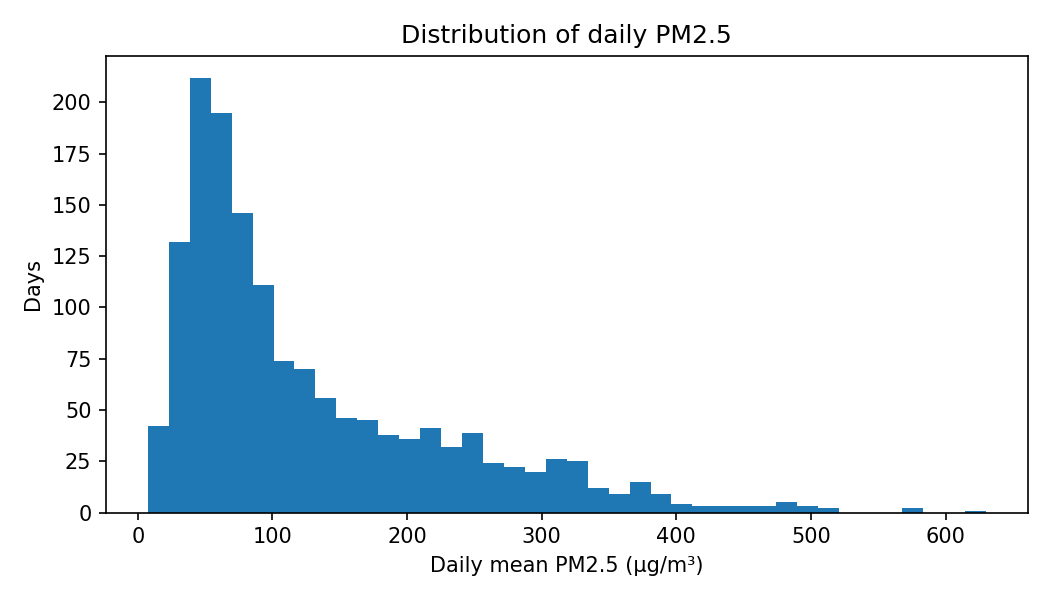
\includegraphics[width=0.78\textwidth]{pm25_distribution.png}
\caption{Distribution of daily mean PM$_{2.5}$ for usable days, Lahore 2019--2025.}
\label{fig:dist}
\end{figure}

\begin{figure}[htbp]
\centering
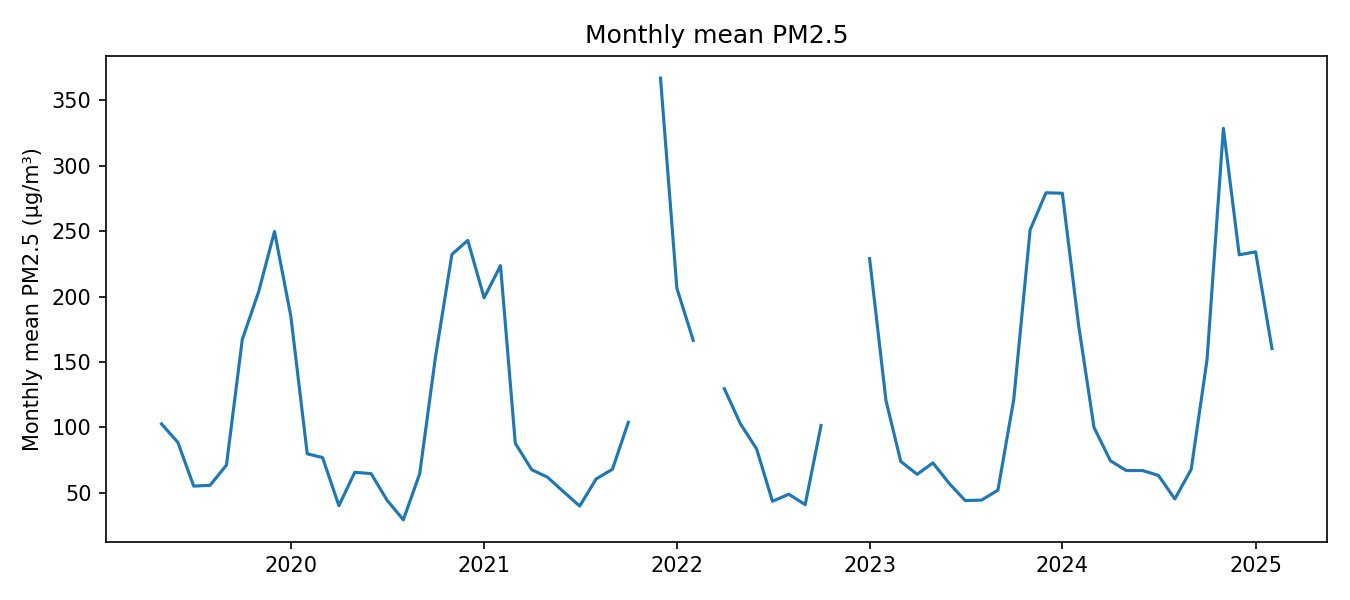
\includegraphics[width=0.86\textwidth]{pm25_monthly.png}
\caption{Monthly mean PM$_{2.5}$. The winter peaks dominate the series; gaps are months with too few usable days.}
\label{fig:monthly}
\end{figure}

\paragraph{Data coverage.}
Coverage is uneven. Figure~\ref{fig:coverage} shows the percentage of usable days in each month: some months are complete, while parts of 2022 and 2023 have very few usable days. This matters for evaluation, because a model trained mostly on winter smog will see a different mix of conditions in a sparse summer month. The time-based split and the per-season error analysis in Phase~3 are designed with this in mind.

\begin{figure}[htbp]
\centering
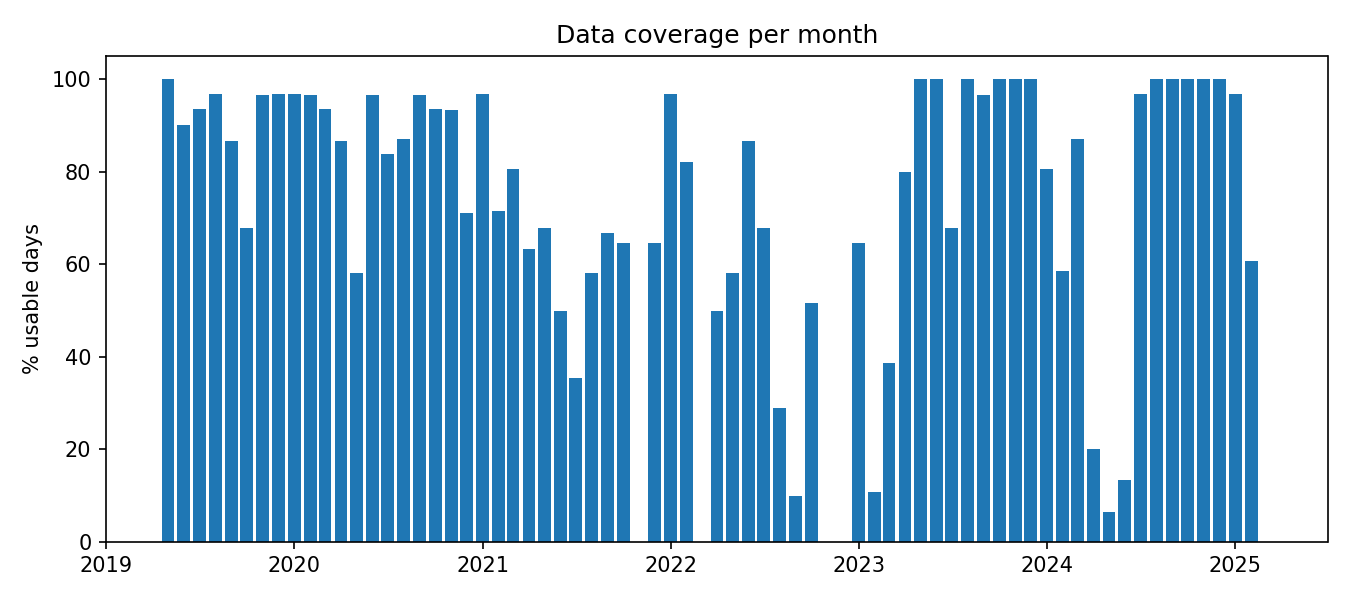
\includegraphics[width=0.86\textwidth]{coverage_by_month.png}
\caption{Percentage of usable days per month. Gaps are months with insufficient valid hourly readings.}
\label{fig:coverage}
\end{figure}

\paragraph{AQI categories.}
Figure~\ref{fig:aqi} and Table~\ref{tab:aqi} show the AQI class distribution. ``Unhealthy'' is the most common class (647 days, 43.0\%), and 1{,}102 days (73.2\%) are ``Unhealthy'' or worse. Only 9 days (0.6\%) are ``Good''. The classes are therefore strongly imbalanced, so overall accuracy would be misleading; Phase~3 will report macro-averaged F1 and per-class recall alongside accuracy.

\begin{figure}[htbp]
\centering
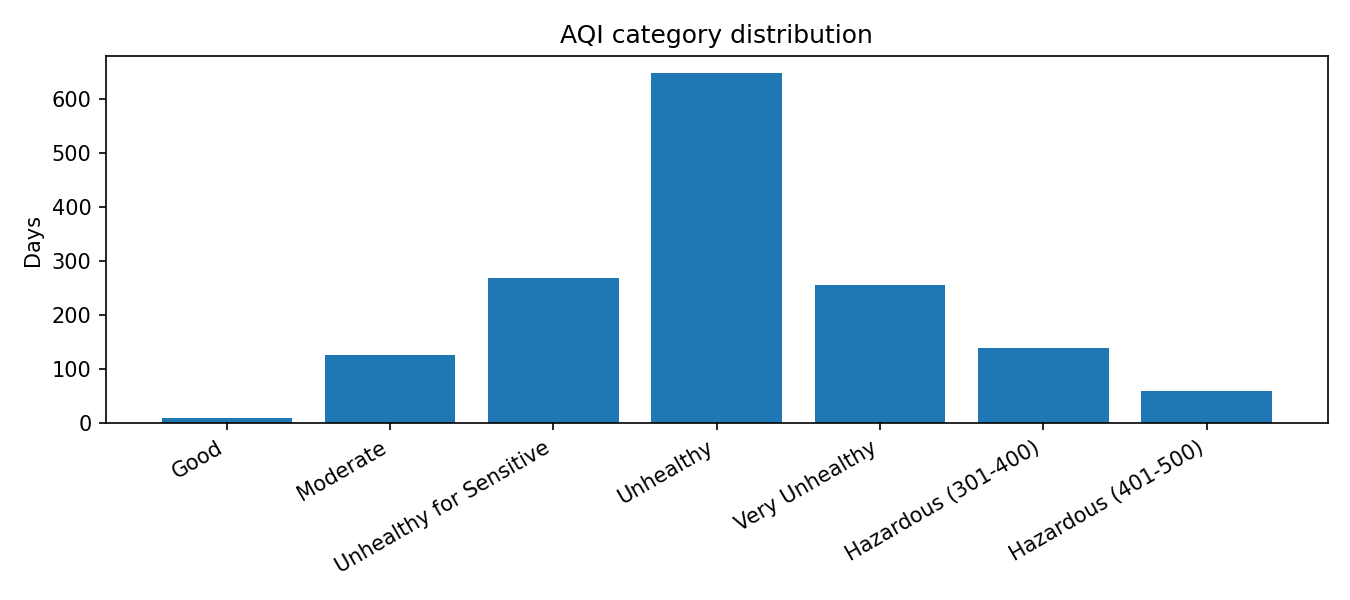
\includegraphics[width=0.86\textwidth]{aqi_class_distribution.png}
\caption{Daily AQI category counts for usable days.}
\label{fig:aqi}
\end{figure}

\begin{table}[htbp]
\centering
\small
\begin{tabular}{L{5.2cm}rr}
\toprule
\textbf{AQI category} & \textbf{Days} & \textbf{Share} \\
\midrule
Good & 9 & 0.6\% \\
Moderate & 126 & 8.4\% \\
Unhealthy for Sensitive Groups & 269 & 17.9\% \\
Unhealthy & 647 & 43.0\% \\
Very Unhealthy & 256 & 17.0\% \\
Hazardous (301--400) & 139 & 9.2\% \\
Hazardous (401--500) & 60 & 4.0\% \\
\midrule
Total & 1{,}506 & 100\% \\
\bottomrule
\end{tabular}
\caption{AQI category distribution for the 1{,}506 usable days.}
\label{tab:aqi}
\end{table}

\paragraph{Relationships with weather.}
Figure~\ref{fig:corr} reports Pearson correlations between daily PM$_{2.5}$ and the meteorological variables. The strongest associations are negative with temperature ($r=-0.64$) and shortwave radiation ($r=-0.50$), and positive with surface pressure ($r=+0.64$). Wind speed is negatively associated ($r=-0.38$) and humidity positively ($r=+0.30$). Figure~\ref{fig:weather} shows the same relationships as scatter plots with linear fits. These patterns are physically consistent: cold, calm, high-pressure days with weak sunlight and little ventilation allow pollution to accumulate, while wind and rain disperse it.

\begin{figure}[htbp]
\centering
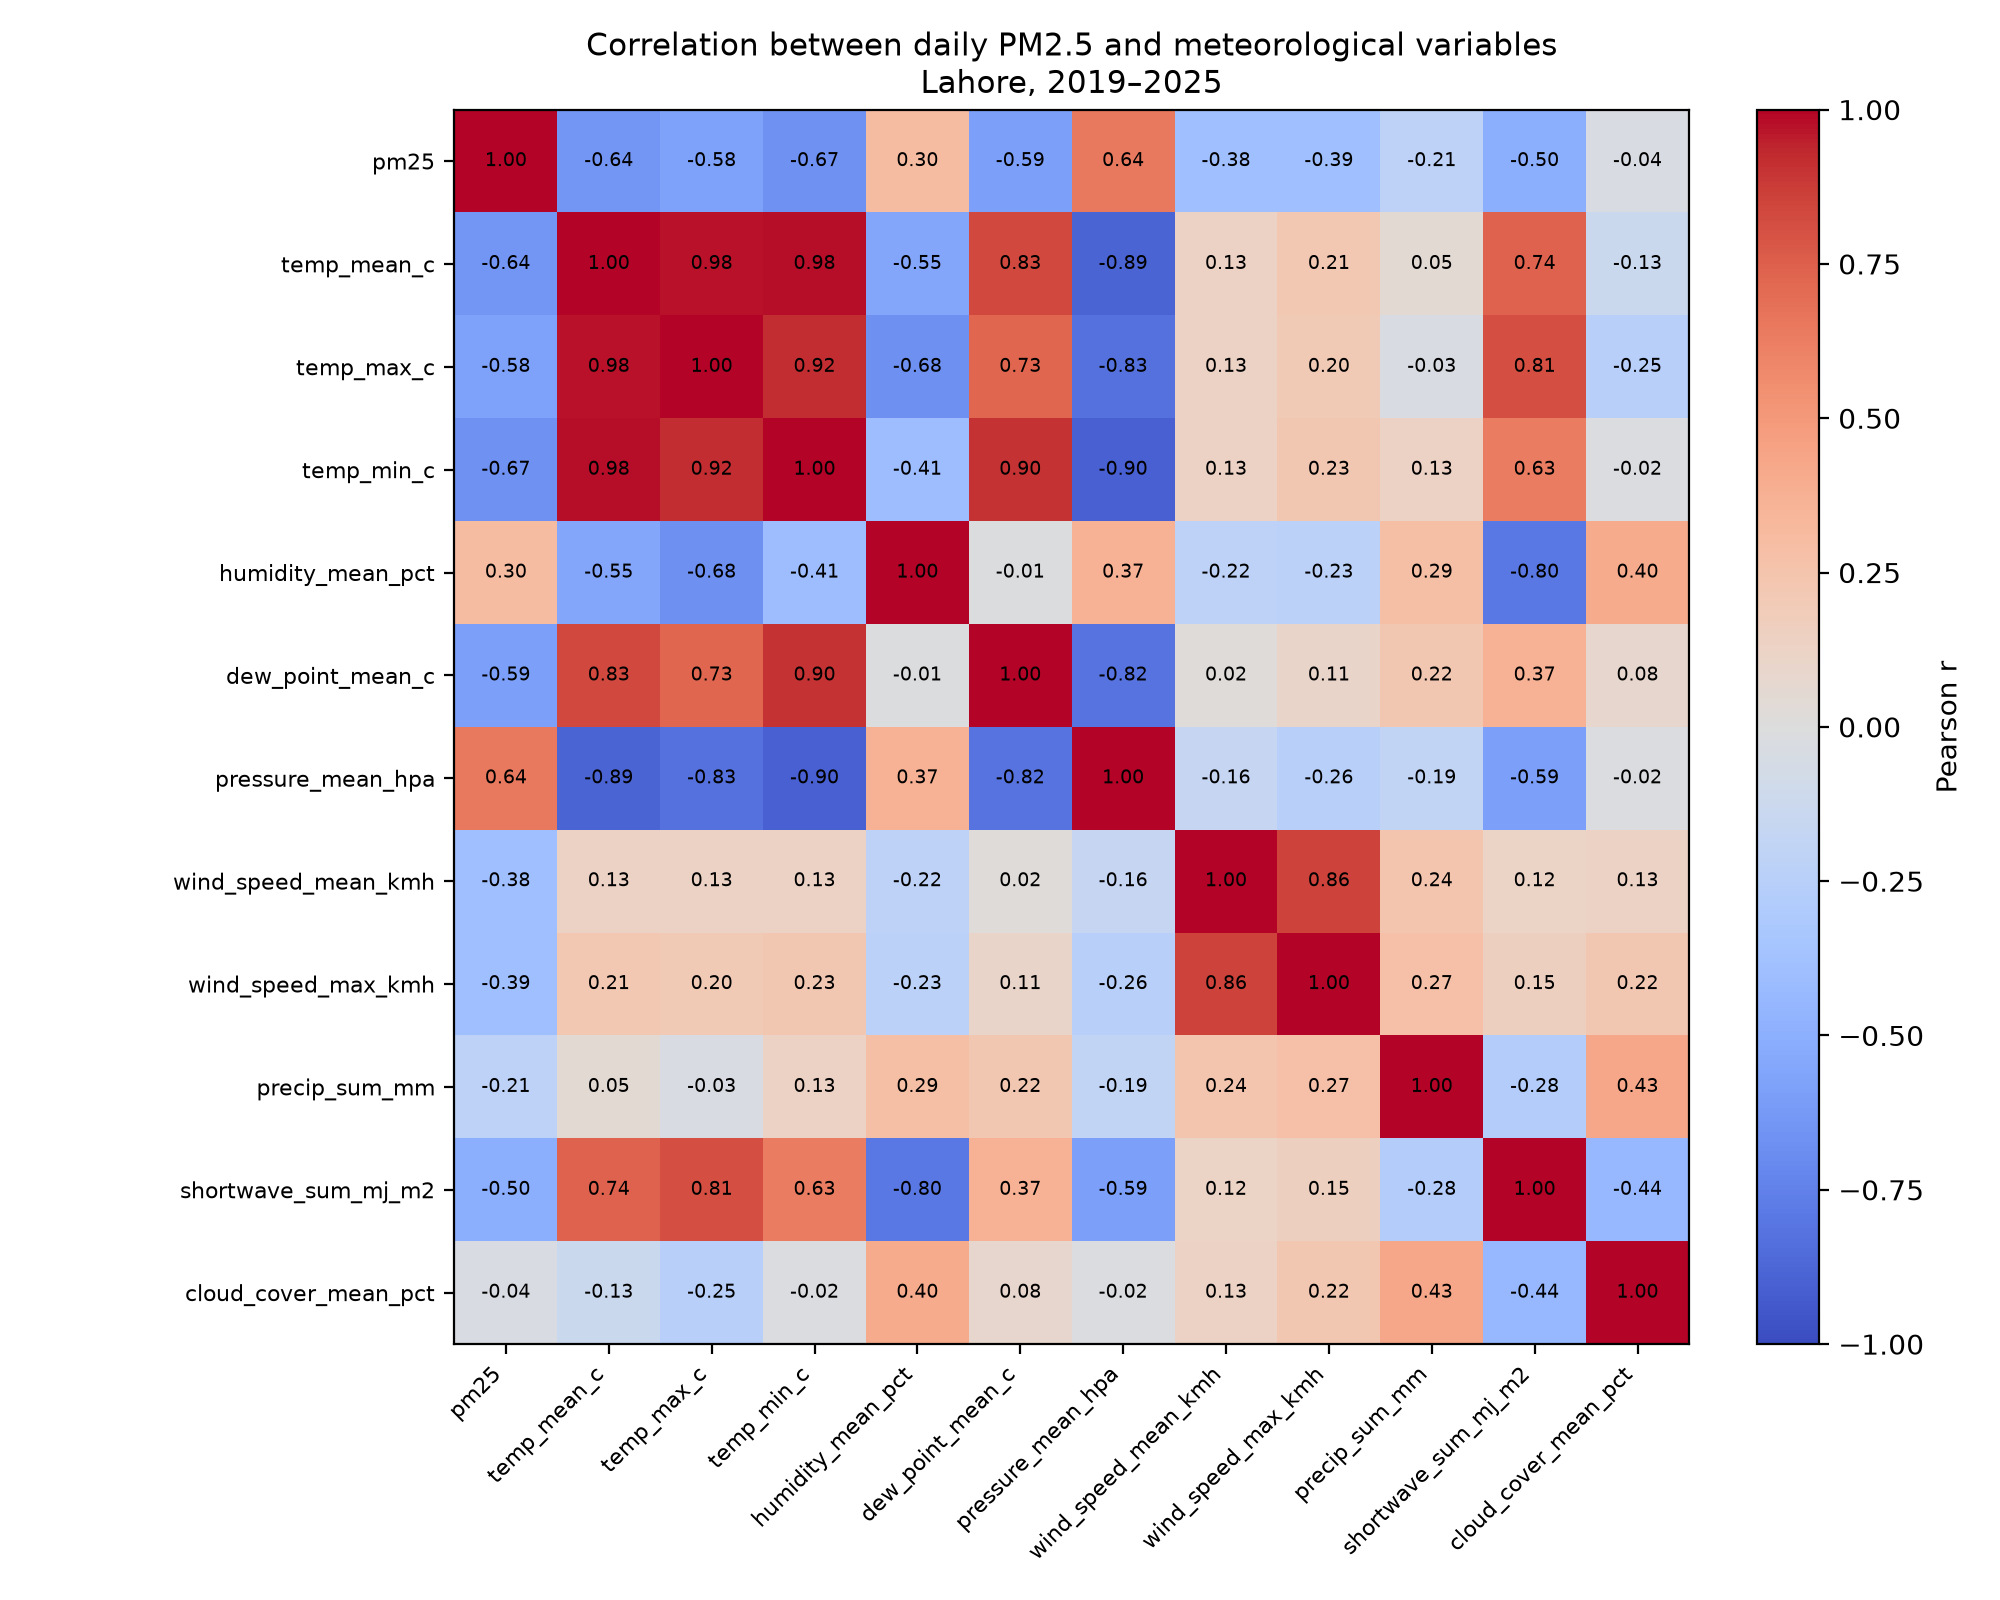
\includegraphics[width=0.86\textwidth]{correlation_heatmap.png}
\caption{Pearson correlation matrix for daily PM$_{2.5}$ and meteorological variables.}
\label{fig:corr}
\end{figure}

\begin{figure}[htbp]
\centering
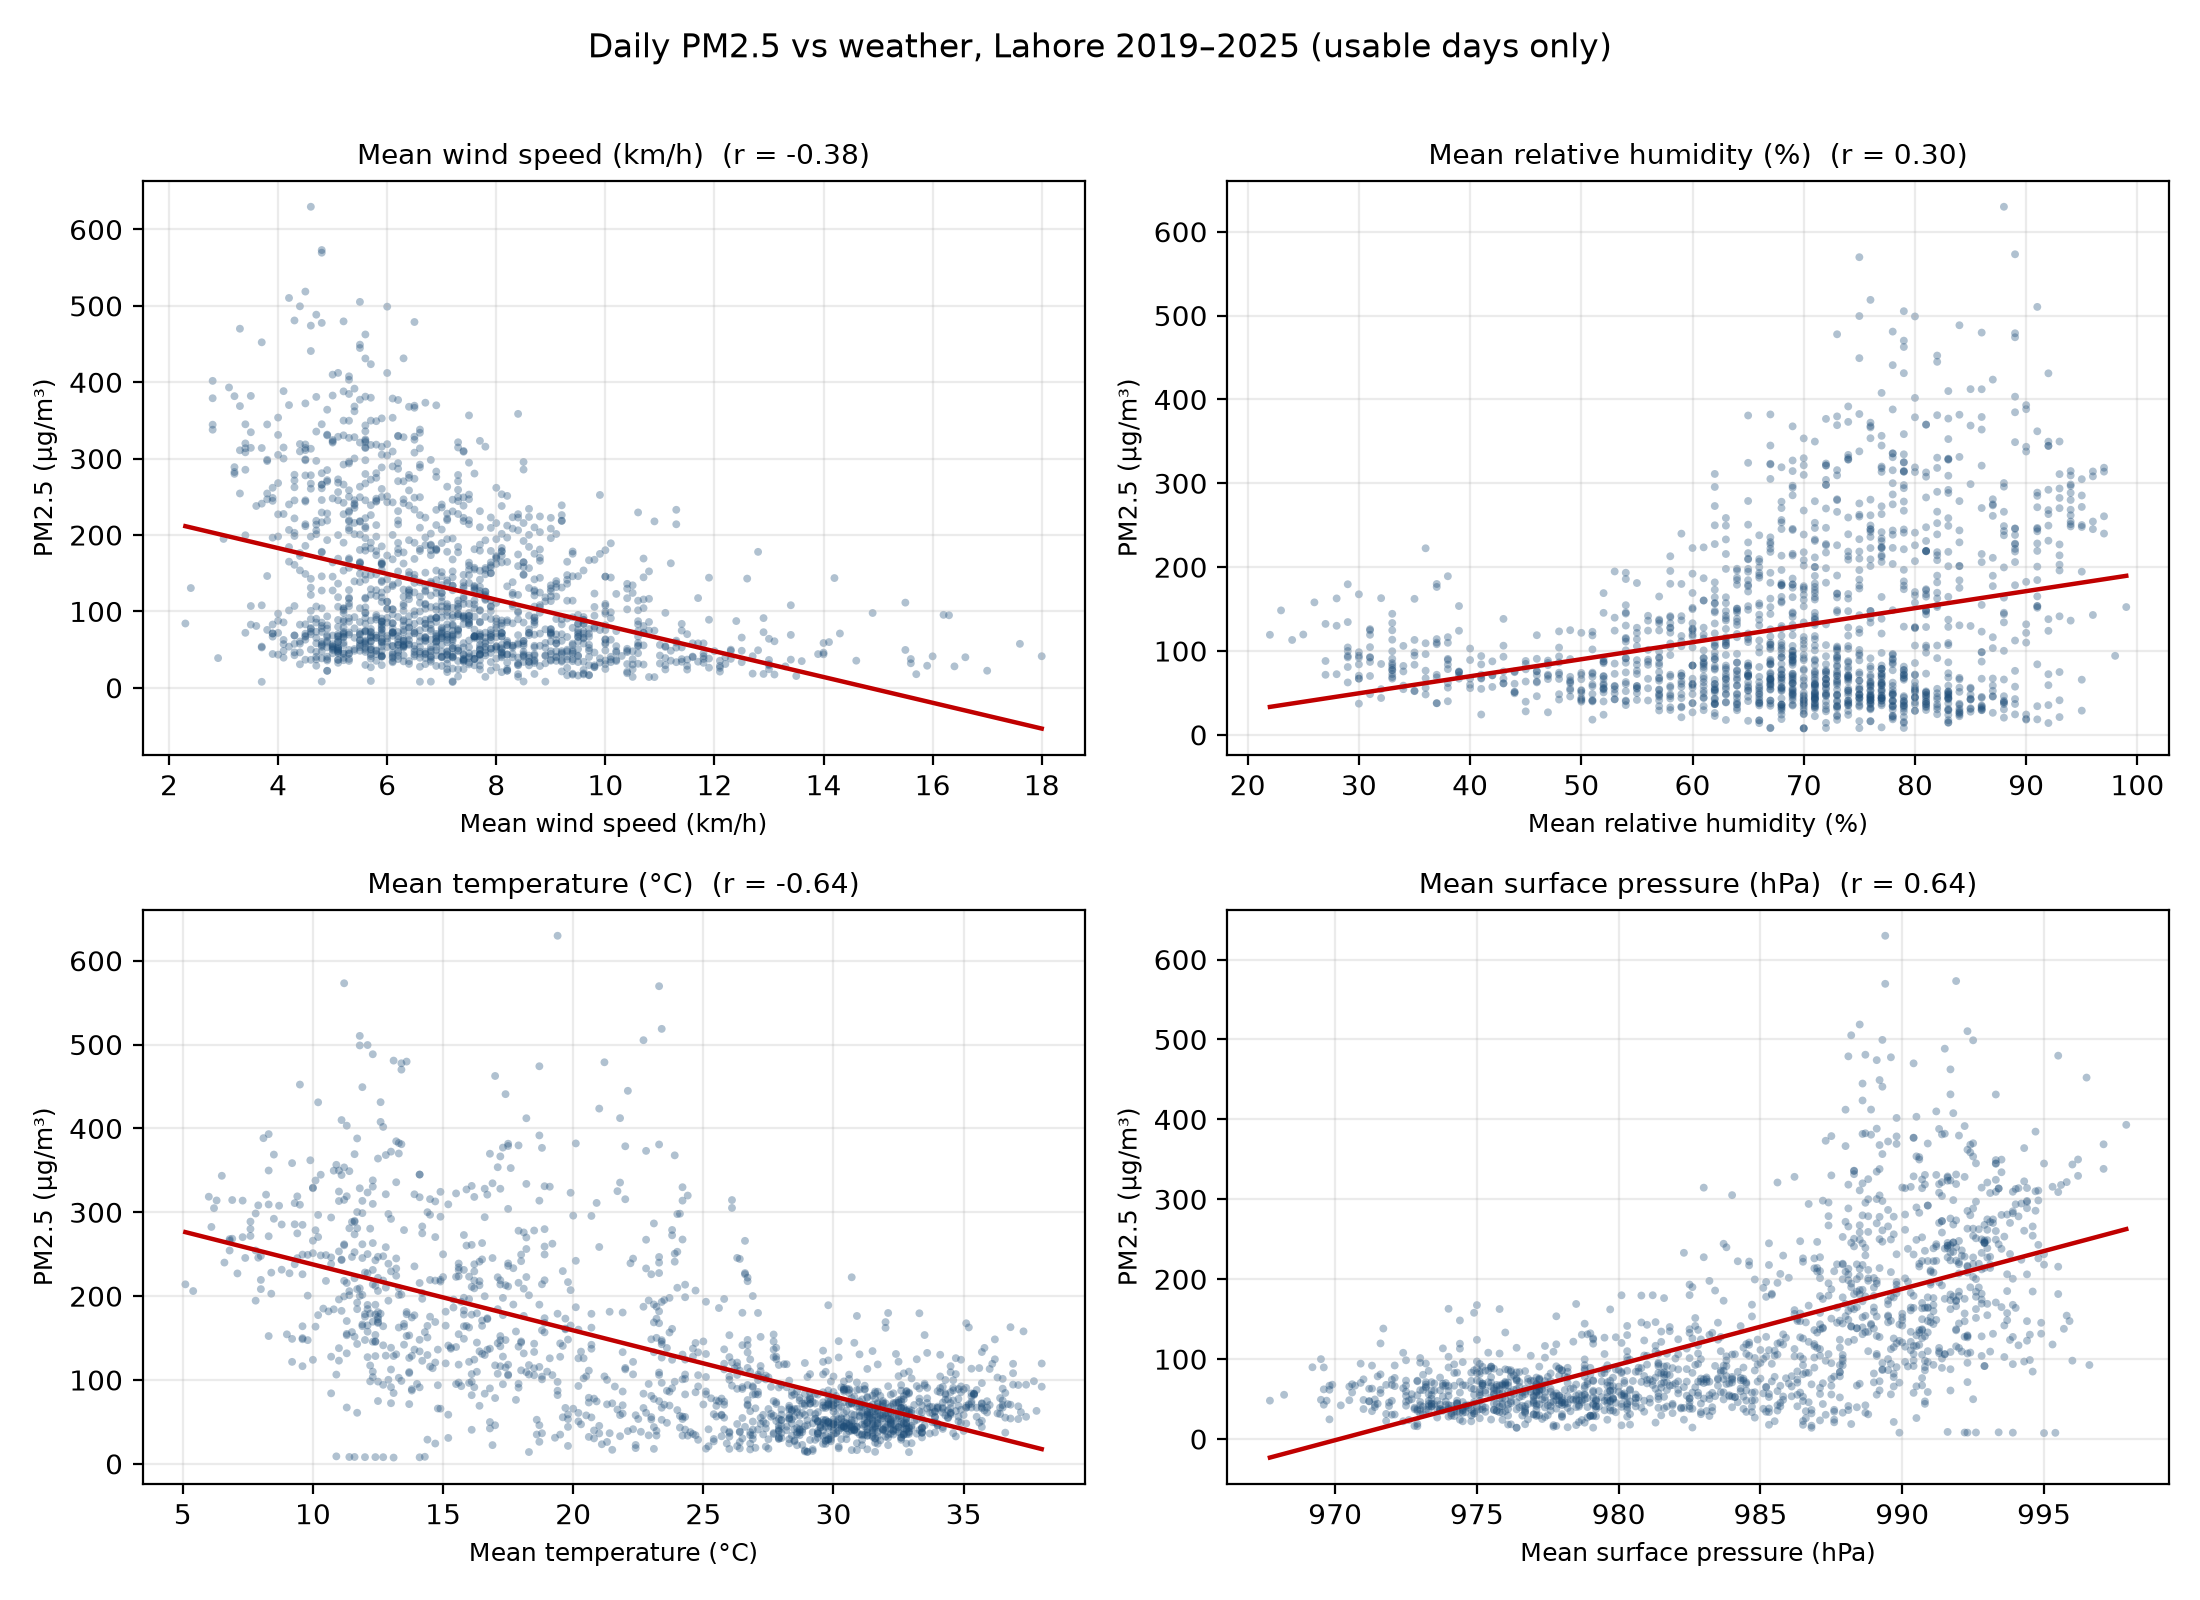
\includegraphics[width=0.92\textwidth]{weather_vs_pm25.png}
\caption{Daily PM$_{2.5}$ against wind speed, humidity, temperature and pressure, with linear fits.}
\label{fig:weather}
\end{figure}

\paragraph{What the EDA implies for modelling.}
Three points follow. First, the seasonal cycle is strong enough that season and calendar features are necessary, not optional. Second, persistence is likely to be the hardest baseline to beat, which is why Phase~1 commits to reporting it. Third, the weather relationships are correlations, not causal effects; the models will be evaluated on held-out years rather than on their ability to fit these patterns.

\subsection{Data Limitations and Ethical Considerations}

\begin{itemize}
  \item \textbf{One monitor, not a city.} The target comes from a single US Diplomatic Post monitor. It is a useful reference series but does not represent every neighbourhood in Lahore.
  \item \textbf{Substantial gaps.} 607 of 2{,}113 calendar days (28.7\%) do not have enough valid hours. Coverage is uneven across months, so evaluation must report results by season as well as overall.
  \item \textbf{Station file gaps.} The station AQI is missing on 221 of 1{,}644 days (13.4\%), including a 47-day gap in the 2021 smog season.
  \item \textbf{Modelled data is not measured data.} The CAMS products are used for comparison only. On the 632 days shared with the monitor, the modelled daily series averaged 0.54 of the monitor's level (median daily ratio 0.61) and under-read smog peaks, so it cannot substitute for observations.
  \item \textbf{Calendar proxies are approximate.} Ramadan and Eid dates follow published calendars but can shift by a day with moon sighting; public holidays are a simplification. Traffic is not observed directly.
  \item \textbf{Licences.} The Zenodo dataset is CC0-1.0 and Open-Meteo/ERA5 is CC BY 4.0. The Kaggle \texttt{aadbutt} dataset states an unknown licence, and the GitHub station repository states no licence. We therefore attribute both sources and keep raw files out of the public repository rather than redistributing them.
  \item \textbf{Not medical advice.} The application provides cautious, category-based guidance and does not replace official health advisories.
\end{itemize}

% Phase 3 and Phase 4 body, extracted from final_work_deliverable_2/report_d2.tex.
% Table paths are adjusted for the report/ build directory.
% The scientific content and numbers are unchanged from Deliverable 2.
\section{Phase 3: Models, baselines, and selection protocol}

\subsection{Classification}

The classification candidates were:

\begin{enumerate}[leftmargin=1.4em]
  \item Majority class.
  \item Persistence: tomorrow's category equals today's category.
  \item Logistic regression with class weights.
  \item Histogram gradient boosting (HGB).
  \item An optional small MLP, retained only if it improved validation performance.
\end{enumerate}

The persistence baseline uses the majority training class code, 2 (Unhealthy), as its fallback when today's category is missing. This fallback must be stated whenever the persistence result is reported. The MLP was excluded after validation macro F1 of 0.4124 did not exceed HGB's 0.4941.

Hyperparameters were tuned with five-fold \texttt{TimeSeriesSplit} on the raw training frame, with a seven-day gap. Tuning never cross-validated on the already-preprocessed training matrix. The final model was refitted on the training split only, not on train plus validation. The test set was then touched once for the final model. The classification selection metric was validation macro F1 over all six configured labels. The CV score is computed per fold over the classes present in that fold, so it is not directly comparable with the six-label validation score; that caveat is recorded in the metrics file.

\begin{table}[htbp]
\centering
\scriptsize
\caption{Selected hyperparameters. Classification used five-fold time-series CV with a seven-day gap and selected on validation macro F1; regression selected on validation RMSE.}
\label{tab:hyperparameters}
\begin{tabular}{llL{5.0cm}L{3.2cm}l}
\toprule
Task & Model & Selected parameters & Validation metric & Status \\
\midrule
Classification & LogisticRegression & \texttt{\{"C": 0.1, "class\_weight": "balanced", "max\_iter": 500, "penalty": "l1"\}} & macro F1 = 0.4665 & completed \\
Classification & HistGradientBoosting & \texttt{\{"l2\_regularization": 0.1, "learning\_rate": 0.1, "max\_iter": 100, "max\_leaf\_nodes": 31, "min\_samples\_leaf": 10\}} & macro F1 = 0.4941 & selected \\
Classification & MLP & \texttt{\{"alpha": 0.01, "early\_stopping": true, "hidden\_layer\_sizes": [128, 64, 32], "learning\_rate": "constant", "max\_iter": 500, "n\_iter\_no\_change": 15, "validation\_fraction": 0.1\}} & macro F1 = 0.4124 & excluded \\
Regression & Ridge & \texttt{\{"alpha": 10.0\}} & RMSE = 45.6916 & not selected \\
Regression & HGB & \texttt{\{"learning\_rate": 0.05, "max\_depth": 3, "max\_iter": 200\}} & RMSE = 45.6243 & selected \\
\bottomrule
\end{tabular}

\end{table}


\subsection{Regression}

The regression candidates were persistence, Ridge regression, and histogram gradient boosting. Hyperparameters were tuned with the same five-fold time-series procedure and a seven-day gap. Model selection used validation RMSE. The selected model was refitted on training rows only and evaluated once on test. Persistence is not imputed for missing current-day PM2.5; it is scored on the same scorable rows as the models. The final code calls the metric helper with \texttt{allow\_missing=False} for every method. The option \texttt{allow\_missing=True} remains reserved for an unfiltered persistence baseline only; the persistence \texttt{n\_dropped} values are 6 validation and 1 test, the same rows on which every method is scored.

The selected regression model was HGB, with validation RMSE 45.6243; Ridge was close behind at 45.6916. The test comparison is reported in Section~\ref{sec:reg-results} without changing the selection rule.

\section{Phase 3: Classification results}
\label{sec:clf-results}

Table~\ref{tab:clf-metrics} reports validation and test metrics for the majority, persistence, logistic regression, and HGB candidates. HGB was selected on validation macro F1 (0.4941 versus 0.4665 for logistic regression). On test, HGB reached macro F1 0.4780, below persistence's 0.5157. HGB's test accuracy was higher than persistence (0.5856 versus 0.5676), but accuracy is dominated by the larger classes; macro F1 exposes the weaker performance on rare classes.

\begin{table}[htbp]
\centering
\scriptsize
\caption{Classification results on the chronological validation and test splits. Macro F1 is the selection metric.}
\label{tab:clf-metrics}
\begin{tabular}{llrrrrrrr}
\toprule
Model & Split & Acc. & Bal. acc. & Macro P & Macro R & Macro F1 & Wtd. F1 & AUC \\
\midrule
Majority class & Validation & 0.3033 & 0.1667 & 0.0505 & 0.1667 & 0.0776 & 0.1411 & -- \\
Majority class & Test & 0.3468 & 0.1667 & 0.0578 & 0.1667 & 0.0858 & 0.1786 & -- \\
Persistence & Validation & 0.5697 & 0.4760 & 0.4772 & 0.4760 & 0.4766 & 0.5691 & -- \\
Persistence & Test & 0.5676 & 0.5157 & 0.5157 & 0.5157 & 0.5157 & 0.5676 & -- \\
Logistic regression & Validation & 0.5287 & 0.4995 & 0.4775 & 0.4995 & 0.4665 & 0.5521 & 0.8842 \\
Logistic regression & Test & 0.5225 & 0.5062 & 0.4673 & 0.5062 & 0.4601 & 0.5337 & 0.8719 \\
\textbf{HGB} & Validation & 0.5943 & 0.4976 & 0.5049 & 0.4976 & 0.4941 & 0.5824 & 0.8765 \\
\textbf{HGB} & Test & 0.5856 & 0.4776 & 0.4804 & 0.4776 & 0.4780 & 0.5815 & 0.8886 \\
\bottomrule
\end{tabular}

\end{table}


The selected HGB model's test AUC-ROC is 0.8886 and logistic regression's is 0.8719. The one-vs-rest macro AUC is computed from the aligned six-column probability matrix. Rows sum to one within the helper's tolerance. The majority baseline has no probability output, so its AUC is reported as undefined rather than filled with a fake value. HGB's test AUC (0.8886) is higher than its validation AUC (0.8765) even though its test macro F1 is below persistence. AUC measures probability ranking rather than the thresholded label decision, and persistence has no probability output, so the two metrics answer different questions. Persistence's test macro precision, recall, and F1 are all 0.5157, and its weighted F1 equals accuracy (0.5676), because predicted and true class counts coincide exactly on the test rows. This is not a copy error; it is a property of the persistence shift on this series.

Table~\ref{tab:clf-per-class} gives the selected HGB model's test per-class results. Good/Moderate has support 8 and Hazardous 401--500 has support 19; both should be read as noisy. The largest class, Unhealthy, has F1 0.7013, while Very Unhealthy has F1 0.7040. The two Hazardous bands are weaker: 0.3600 and 0.2353.

\begin{table}[htbp]
\centering
\small
\caption{Per-class test performance of the selected HistGradientBoosting classifier. Good/Moderate and Hazardous (401--500) have small support and should be treated as noisy estimates.}
\label{tab:clf-per-class}
\begin{tabular}{lrrrr}
\toprule
Category & Support & Precision & Recall & F1 \\
\midrule
Good/Moderate & 8 & 0.3750 & 0.3750 & 0.3750 \\
Unhealthy for Sensitive & 34 & 0.5161 & 0.4706 & 0.4923 \\
Unhealthy & 77 & 0.7013 & 0.7013 & 0.7013 \\
Very Unhealthy & 60 & 0.6769 & 0.7333 & 0.7040 \\
Hazardous (301-400) & 24 & 0.3462 & 0.3750 & 0.3600 \\
Hazardous (401-500) & 19 & 0.2667 & 0.2105 & 0.2353 \\
\bottomrule
\end{tabular}

\end{table}


Table~\ref{tab:clf-confusion} gives the test confusion matrix. The model frequently predicts Unhealthy when the truth is Unhealthy for Sensitive, and it confuses the two Hazardous bands with each other and with Very Unhealthy. This is consistent with ordered severity classes and with the class imbalance.

\begin{table}[htbp]
\centering
\scriptsize
\caption{Selected HGB test confusion matrix. Codes: 0 Good/Moderate, 1 Unhealthy for Sensitive, 2 Unhealthy, 3 Very Unhealthy, 4 Hazardous (301--400), 5 Hazardous (401--500).}
\label{tab:clf-confusion}
\begin{tabular}{lrrrrrr}
\toprule
True & Pred 0 & Pred 1 & Pred 2 & Pred 3 & Pred 4 & Pred 5 \\
\midrule
0 & 3 & 2 & 3 & 0 & 0 & 0 \\
1 & 4 & 16 & 14 & 0 & 0 & 0 \\
2 & 1 & 13 & 54 & 6 & 2 & 1 \\
3 & 0 & 0 & 6 & 44 & 7 & 3 \\
4 & 0 & 0 & 0 & 8 & 9 & 7 \\
5 & 0 & 0 & 0 & 7 & 8 & 4 \\
\bottomrule
\end{tabular}

\end{table}


\begin{figure}[htbp]
  \centering
  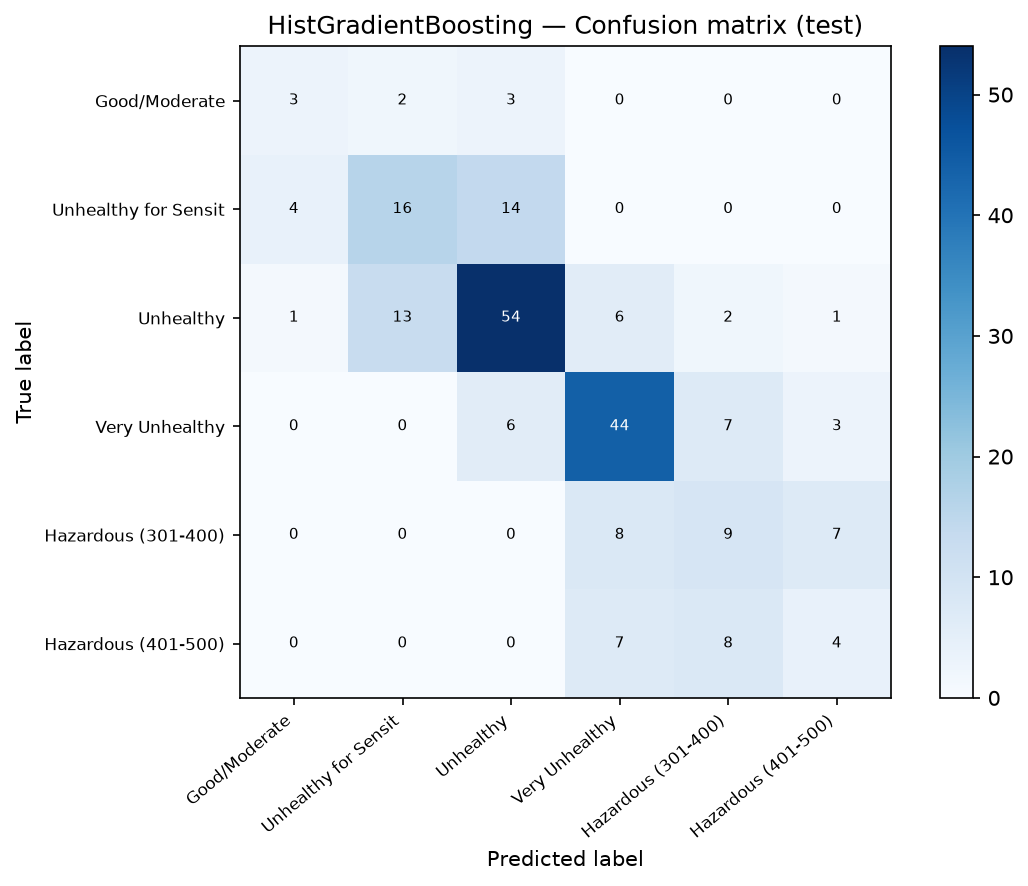
\includegraphics[width=0.82\linewidth]{classification_confusion_histgradientboosting_test.png}
  \caption{Selected HGB test confusion matrix. The raw matrix is also given in Table~\ref{tab:clf-confusion}.}
  \label{fig:clf-confusion}
\end{figure}

\begin{figure}[htbp]
  \centering
  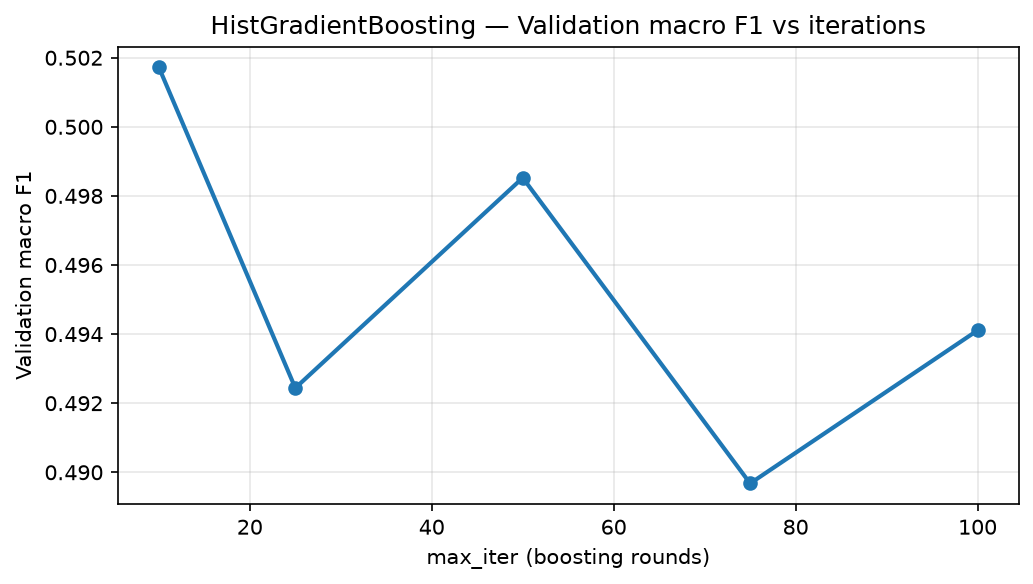
\includegraphics[width=0.82\linewidth]{classification_hgb_val_curve.png}
  \caption{Validation macro F1 for the HGB configuration used in model selection.}
  \label{fig:clf-curve}
\end{figure}

\begin{figure}[htbp]
  \centering
  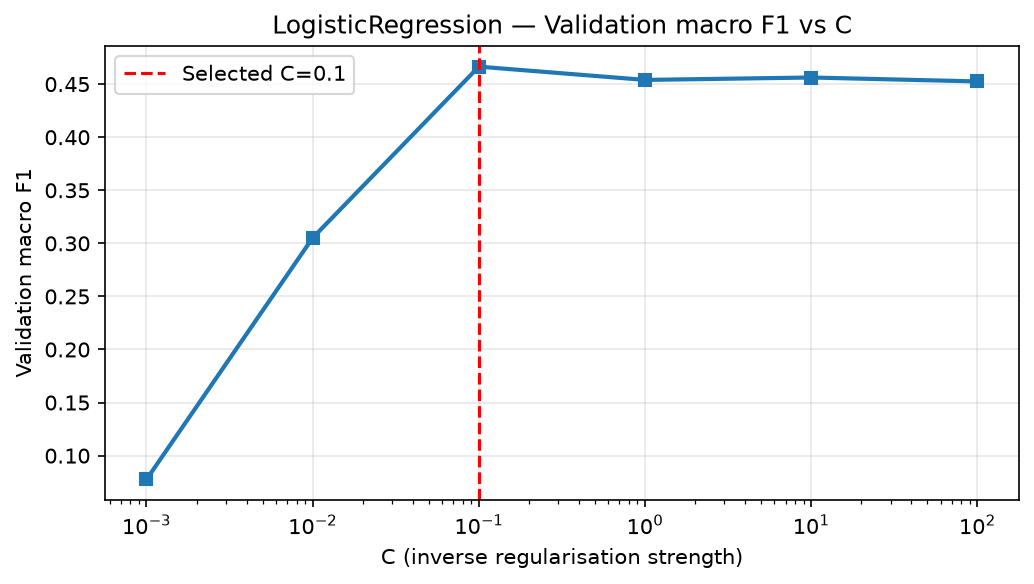
\includegraphics[width=0.78\linewidth]{classification_lr_C_curve.png}
  \caption{Logistic-regression validation curve over the regularisation strength $C$. The selected value was $C=0.1$.}
  \label{fig:clf-c}
\end{figure}

\paragraph{Training curves.} A per-epoch training-loss curve exists only for the MLP, which was excluded because its validation macro F1 (0.4124) did not exceed that of HGB (0.4941). For logistic regression (full-batch solver) and HGB (no per-epoch loss recorded in our configuration) we report validation-score curves instead (Figures~\ref{fig:clf-curve}, \ref{fig:clf-c}, and \ref{fig:reg-learning}). Figure~\ref{fig:clf-curve} is nearly flat (macro F1 between about 0.490 and 0.502), so the iteration count is not a sensitive parameter.

\section{Phase 3: Regression results}
\label{sec:reg-results}

Table~\ref{tab:reg-metrics} reports the regression comparison. On validation, HGB had the lowest RMSE (45.6243), narrowly ahead of Ridge (45.6916); both beat persistence (51.5457) by about 11.4--11.5\%. On test, however, HGB reached 64.9198, essentially tied with persistence (64.8175, a 0.10 RMSE gap); its skill score was $-0.0016$. Ridge reached 62.0956 on test and beat persistence, with skill 0.0420. R2 follows the same pattern: Ridge's test $R^2$ is 0.7356, HGB's is 0.7110, and persistence's is 0.7119.

This is a genuine validation-to-test reversal, not a reporting error. The selection rule chose HGB on validation RMSE before test was touched. The report keeps that selection and reports the test outcome honestly. It does not switch the final model to Ridge after seeing test.

\begin{table}[htbp]
\centering
\small
\caption{Regression results on the chronological validation and test splits. Skill is $1-\mathrm{RMSE}_{model}/\mathrm{RMSE}_{persistence}$.}
\label{tab:reg-metrics}
\begin{tabular}{llrrrrr}
\toprule
Model & Split & RMSE & MAE & $R^2$ & Skill & $n$ \\
\midrule
Persistence & Validation & 51.5457 & 33.5298 & 0.7808 & -- & 244 \\
Persistence & Test & 64.8175 & 39.9777 & 0.7119 & -- & 222 \\
Ridge & Validation & 45.6916 & 31.8794 & 0.8277 & 0.1136 & 244 \\
Ridge & Test & 62.0956 & 38.4750 & 0.7356 & 0.0420 & 222 \\
\textbf{HGB} & Validation & 45.6243 & 29.9781 & 0.8282 & 0.1149 & 244 \\
\textbf{HGB} & Test & 64.9198 & 40.7740 & 0.7110 & -0.0016 & 222 \\
\bottomrule
\end{tabular}

\end{table}


All models are scored on the same 244 validation and 222 test scorable rows; the 6 validation and 1 test rows dropped for missing current-day PM2.5 are not scored.

\begin{figure}[htbp]
  \centering
  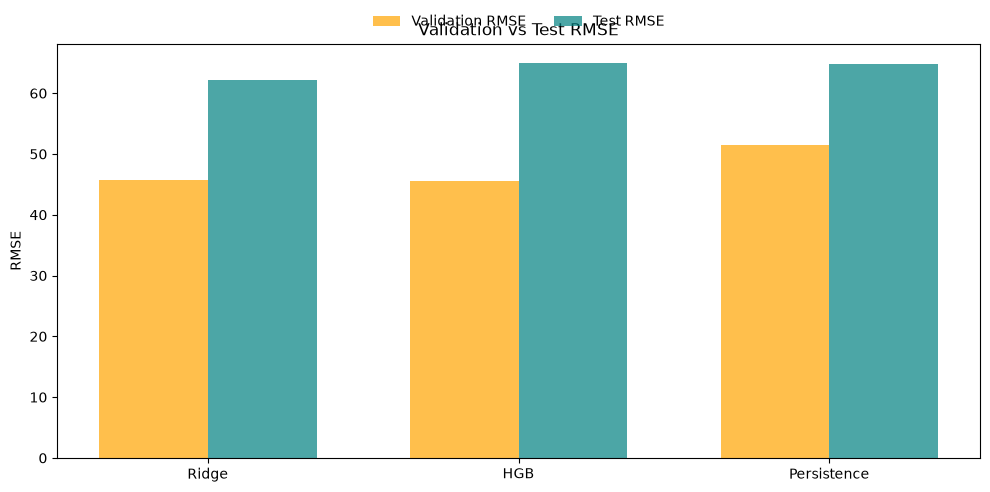
\includegraphics[width=0.82\linewidth]{regression_metric_comparison.png}
  \caption{Regression metric comparison across candidate models and splits.}
  \label{fig:reg-comparison}
\end{figure}

\begin{figure}[htbp]
  \centering
  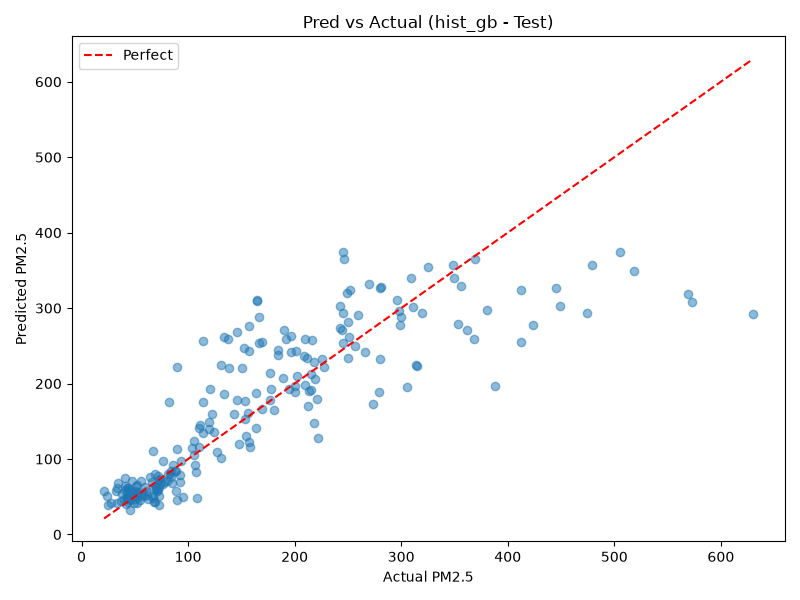
\includegraphics[width=0.9\linewidth]{regression_hist_gb_pred_vs_actual.png}
  \caption{Selected HGB regression: predicted versus actual next-day PM2.5.}
  \label{fig:reg-pred}
\end{figure}

\begin{figure}[htbp]
  \centering
  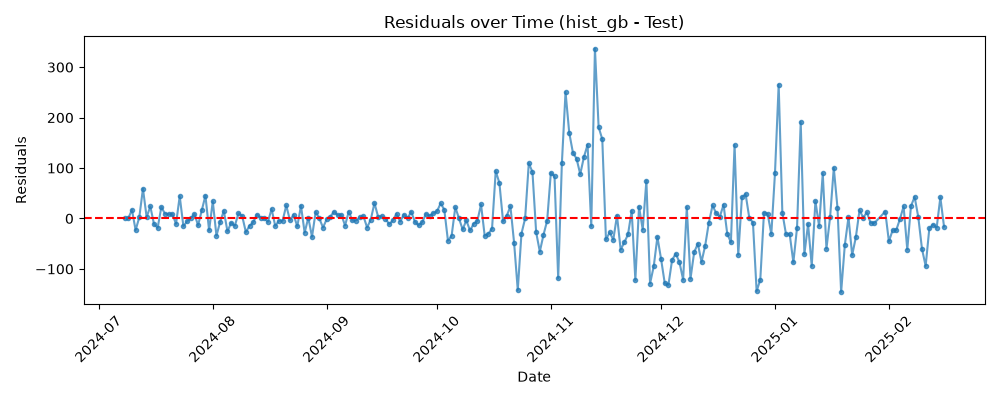
\includegraphics[width=0.9\linewidth]{regression_hist_gb_residuals_over_time.png}
  \caption{Selected HGB regression residuals over time.}
  \label{fig:reg-resid-time}
\end{figure}

\begin{figure}[htbp]
  \centering
  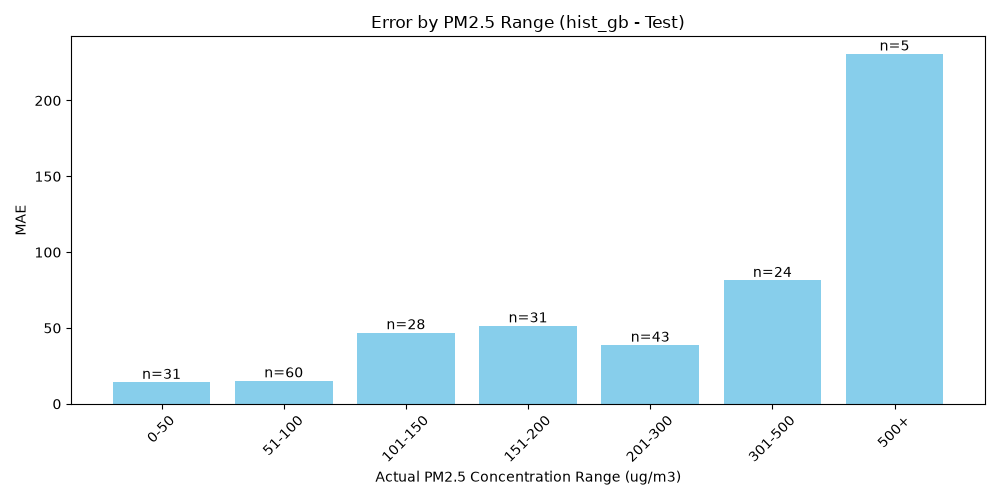
\includegraphics[width=0.82\linewidth]{regression_hist_gb_error_by_severity.png}
  \caption{Selected HGB regression error by pollution severity.}
  \label{fig:reg-severity}
\end{figure}

\begin{figure}[htbp]
  \centering
  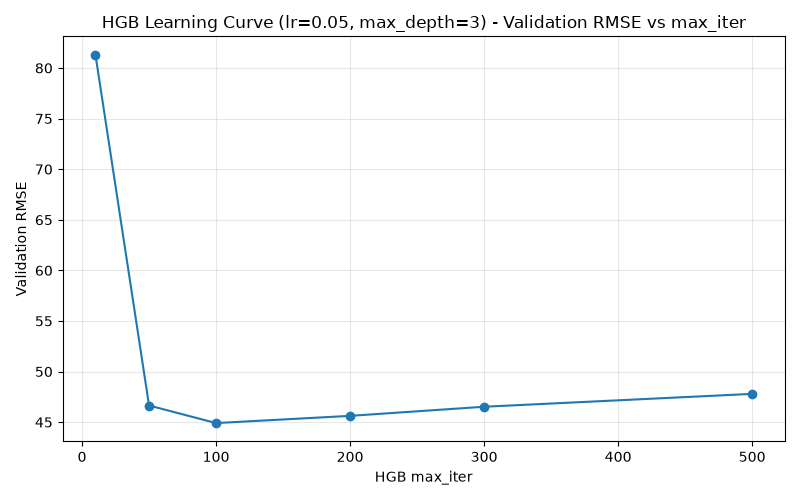
\includegraphics[width=0.82\linewidth]{regression_hgb_learning_curve.png}
  \caption{HGB regression learning curve used as training diagnostic material.}
  \label{fig:reg-learning}
\end{figure}

\section{Phase 4: Bias and error analysis}

The bias analysis joins the final regression and classification predictions on date and split. It uses 466 joined rows: 244 validation and 222 test. The subgroup table has 47 rows across seven dimensions: AQI category, season, year, weekday versus weekend, Islamic events, public holidays, and PM2.5 severity band. Missing subgroup keys were counted per split and dimension; all counts were zero in the final join.

The joined validation rows contain 25 scorable Ramadan rows and no scorable Eid rows. The feature table flags Eid on 10--12 April and 17--19 June 2024, but the AQI label is missing on those dates; all six dates also lack a next-day target, so they never enter the split. This is a label-coverage limitation, not a calendar-flag gap. The test split has only one Islamic-event group, \texttt{Normal}; no test Ramadan or Eid comparison is therefore possible. Public-holiday test rows number only seven, so the holiday result is marked as small-support. The analysis is environmental and temporal, not demographic: the dataset has one monitoring station and no demographic attributes. It cannot establish fairness across people or neighbourhoods.

\begin{table}[htbp]
\centering
\small
\caption{Missing subgroup keys after joining regression and classification predictions.}
\label{tab:bias-missing}
\begin{tabular}{lrr}
\toprule
Dimension & Validation missing & Test missing \\
\midrule
AQI Category & 0 & 0 \\
Islamic\_Event & 0 & 0 \\
Public\_Holiday & 0 & 0 \\
Season & 0 & 0 \\
Severity\_Band & 0 & 0 \\
Weekday\_Weekend & 0 & 0 \\
Year & 0 & 0 \\
\bottomrule
\end{tabular}

\end{table}


Table~\ref{tab:bias-test} reports the test subgroups. Positive signed error is $y_{true}-y_{pred}$, so a positive value means under-prediction relative to the observed PM2.5. The most important pattern is the severe-pollution tail. Hazardous 401--500 has RMSE 162.14 and signed error 141.70; the 301--500 severity band has RMSE 99.60 and signed error 75.72; and the 500+ band, with only five rows, has RMSE 242.00 and signed error 230.76. These are large errors, not just noise, although the 500+ estimate is unstable because of its tiny support. Severity bands and AQI-category groups are defined by the observed outcome, so high-severity groups look under-predicted and low-severity groups over-predicted partly by construction. The size of the errors (for example RMSE 99.60 on the 301--500 band), not the sign, is the informative result.

Seasonal errors are also uneven. Winter test RMSE is 72.38 with signed error $-17.43$, indicating average over-prediction, while autumn RMSE is 75.32 with signed error $+14.15$, indicating average under-prediction. Summer is much easier (RMSE 19.65). Test 2025 has only 45 rows (1 January--16 February, winter), whereas 2024 has 177 mixed-season rows. The 2025 comparison is therefore confounded with season: RMSE is 69.86 versus 63.60, and macro F1 is 0.4306 versus 0.4832, but this is not a clean temporal comparison. Weekday RMSE is higher than weekend RMSE (68.32 versus 55.64), though weekend macro F1 is lower (0.4276 versus 0.4875).

{\footnotesize
\setlength{\tabcolsep}{4pt}
\begin{longtable}{@{}llrrrrrr@{}}
\caption{Test-set subgroup error and classification performance. Positive signed error means the true value is above the prediction (under-prediction). Small-support groups are marked with $^{*}$.}\label{tab:bias-test}\\
\toprule
Dimension & Group & $n$ & RMSE & MAE & Signed err. & Acc. & Macro F1 \\
\midrule
\endfirsthead
\toprule
Dimension & Group & $n$ & RMSE & MAE & Signed err. & Acc. & Macro F1 \\
\midrule
\endhead
AQI Category & Good/Moderate$^{*}$ & 8 & 25.4601 & 23.6583 & -23.6583 & 0.3750 & 0.5455 \\
AQI Category & Unhealthy for Sensitive & 34 & 12.5892 & 9.8540 & -7.1164 & 0.4706 & 0.6400 \\
AQI Category & Unhealthy & 77 & 43.8019 & 27.9535 & -11.1751 & 0.7013 & 0.8244 \\
AQI Category & Very Unhealthy & 60 & 59.1430 & 44.7748 & -27.9941 & 0.7333 & 0.8462 \\
AQI Category & Hazardous (301-400)$^{*}$ & 24 & 53.2085 & 41.5136 & 11.8486 & 0.3750 & 0.5455 \\
AQI Category & Hazardous (401-500)$^{*}$ & 19 & 162.1417 & 141.6998 & 141.6998 & 0.2105 & 0.3478 \\
Season & Winter & 76 & 72.3755 & 52.6206 & -17.4306 & 0.6053 & 0.4494 \\
Season & Summer & 55 & 19.6486 & 15.0855 & 0.7674 & 0.5091 & 0.4763 \\
Season & Autumn & 91 & 75.3234 & 46.4062 & 14.1519 & 0.6154 & 0.4358 \\
Year & 2024 & 177 & 63.6013 & 39.2136 & 0.7755 & 0.5763 & 0.4832 \\
Year & 2025 & 45 & 69.8649 & 46.9118 & -2.9323 & 0.6222 & 0.4306 \\
Weekday\_Weekend & Weekday & 158 & 68.3224 & 41.7848 & 1.0546 & 0.6139 & 0.4875 \\
Weekday\_Weekend & Weekend & 64 & 55.6356 & 38.2786 & -2.5206 & 0.5156 & 0.4276 \\
Severity\_Band & 0-50 & 31 & 17.6658 & 14.2902 & -12.6398 & 0.4839 & 0.5386 \\
Severity\_Band & 51-100 & 60 & 26.2778 & 15.2874 & 1.1969 & 0.6333 & 0.5302 \\
Severity\_Band & 101-150$^{*}$ & 28 & 61.8758 & 47.0172 & -34.7032 & 0.7143 & 0.8333 \\
Severity\_Band & 151-200 & 31 & 66.9282 & 51.5369 & -42.0886 & 0.8387 & 0.9123 \\
Severity\_Band & 201-300 & 43 & 50.0110 & 38.7876 & -8.5917 & 0.5349 & 0.5635 \\
Severity\_Band & 301-500$^{*}$ & 24 & 99.6015 & 81.4907 & 75.7243 & 0.2083 & 0.2556 \\
Severity\_Band & 500+$^{*}$ & 5 & 242.0043 & 230.7646 & 230.7646 & 0.6000 & 0.7500 \\
Islamic\_Event & Normal & 222 & 64.9198 & 40.7740 & 0.0239 & 0.5856 & 0.4780 \\
Public\_Holiday & Normal & 215 & 65.6586 & 41.4275 & -0.3726 & 0.5767 & 0.4680 \\
Public\_Holiday & Holiday$^{*}$ & 7 & 35.3757 & 20.7040 & 12.2017 & 0.8571 & 0.7333 \\
\bottomrule
\end{longtable}
}


\noindent{\footnotesize\textit{Table note:} Subgroup macro F1 is computed within each subgroup over the true classes present, so it is not comparable across groups or with Table~\ref{tab:clf-metrics}. For AQI Category rows, use accuracy (= recall).\par}

\begin{figure}[htbp]
  \centering
  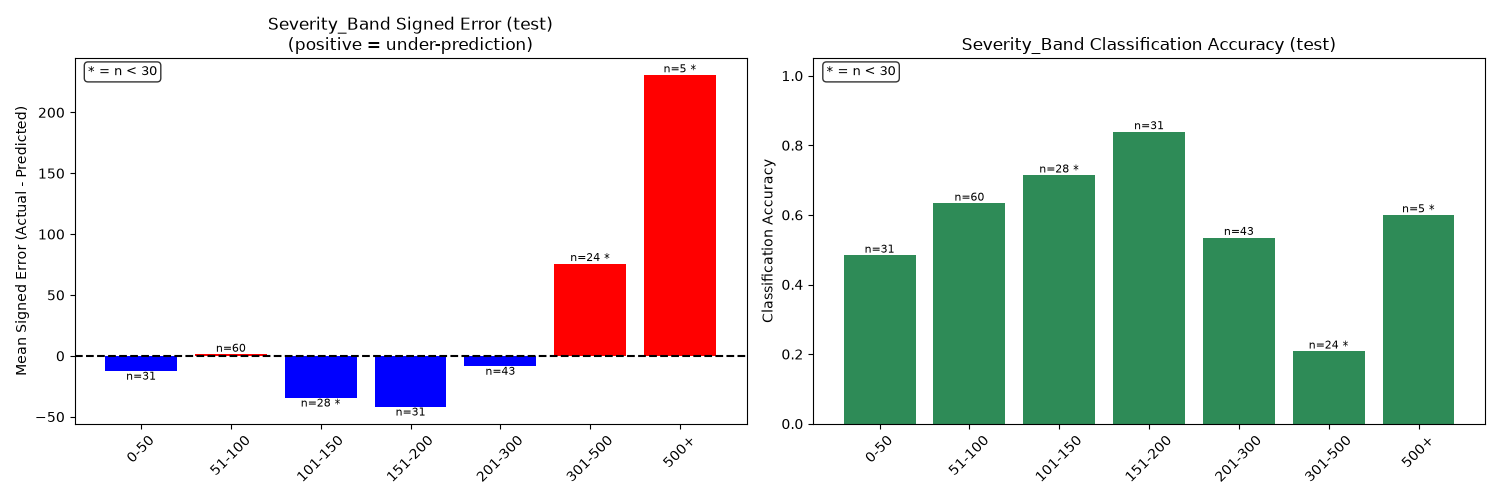
\includegraphics[width=0.95\linewidth]{bias_Severity_Band_test.png}
  \caption{Test signed error and classification accuracy by PM2.5 severity band. Because groups are defined by the observed outcome, the sign is partly constructed; the error magnitude is the informative result. Small groups are marked with an asterisk.}
  \label{fig:bias-severity}
\end{figure}

\begin{figure}[htbp]
  \centering
  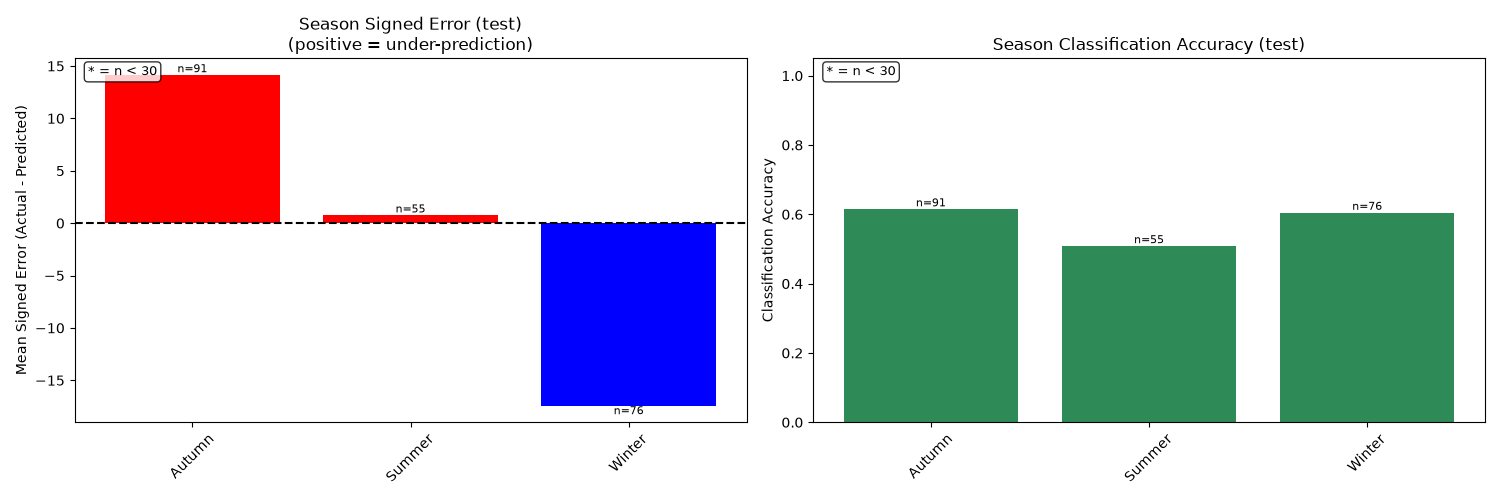
\includegraphics[width=0.95\linewidth]{bias_Season_test.png}
  \caption{Test signed error and classification accuracy by season.}
  \label{fig:bias-season}
\end{figure}

\begin{figure}[htbp]
  \centering
  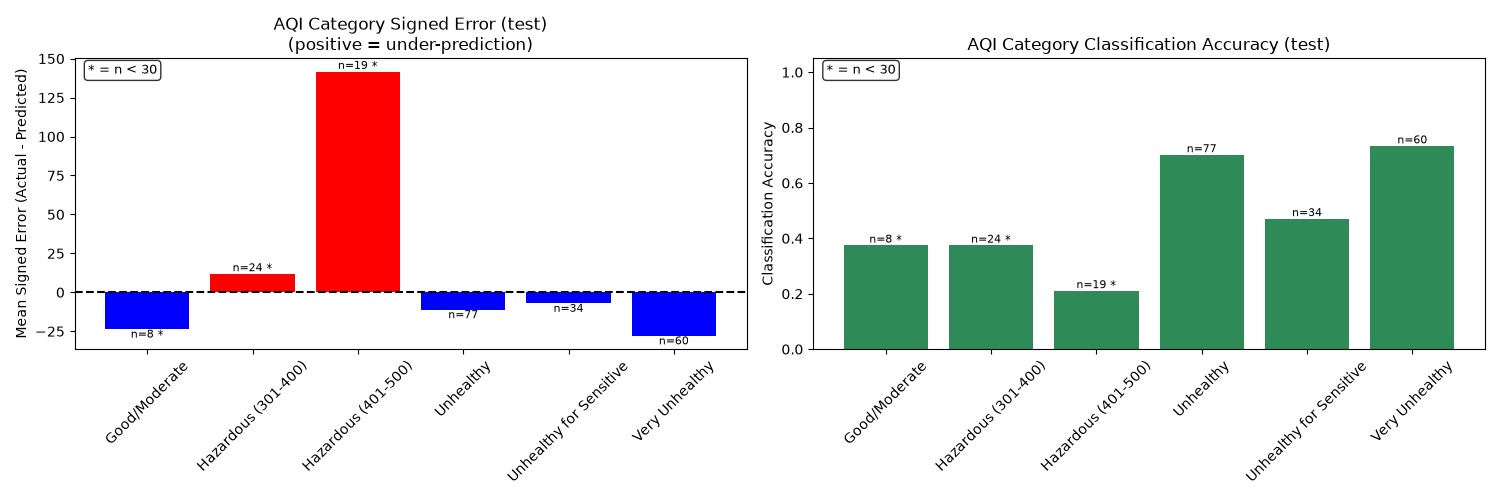
\includegraphics[width=0.95\linewidth]{bias_AQI_Category_test.png}
  \caption{Test signed error and classification accuracy by observed AQI category.}
  \label{fig:bias-aqi}
\end{figure}

\begin{figure}[htbp]
  \centering
  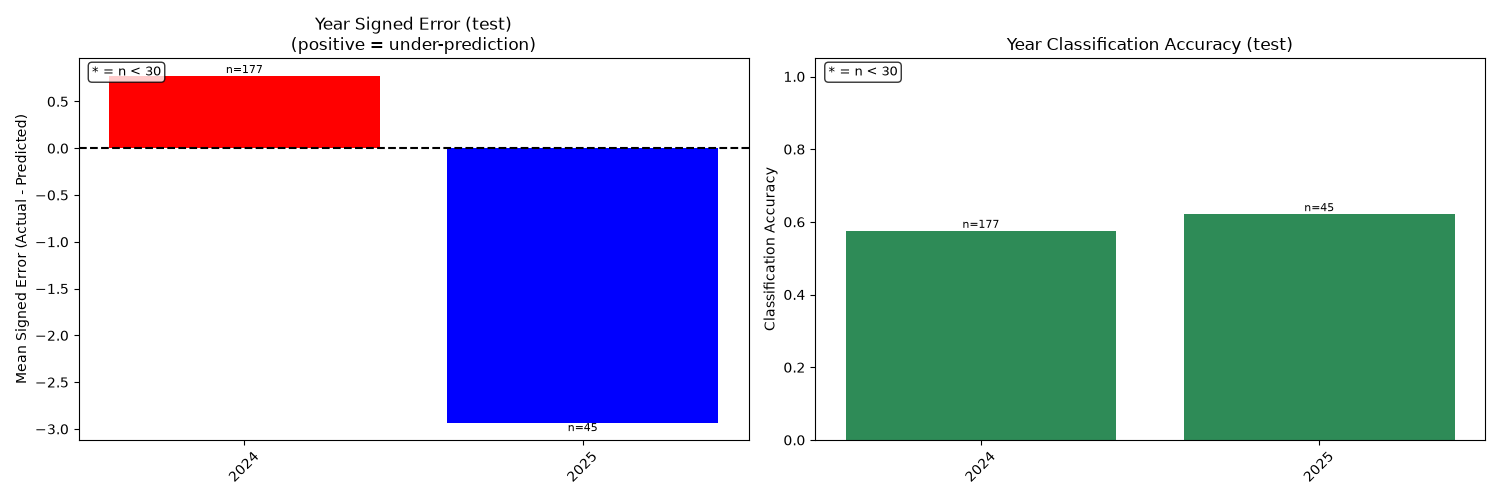
\includegraphics[width=0.95\linewidth]{bias_Year_test.png}
  \caption{Test signed error and classification accuracy by year.}
  \label{fig:bias-year}
\end{figure}

\begin{figure}[htbp]
  \centering
  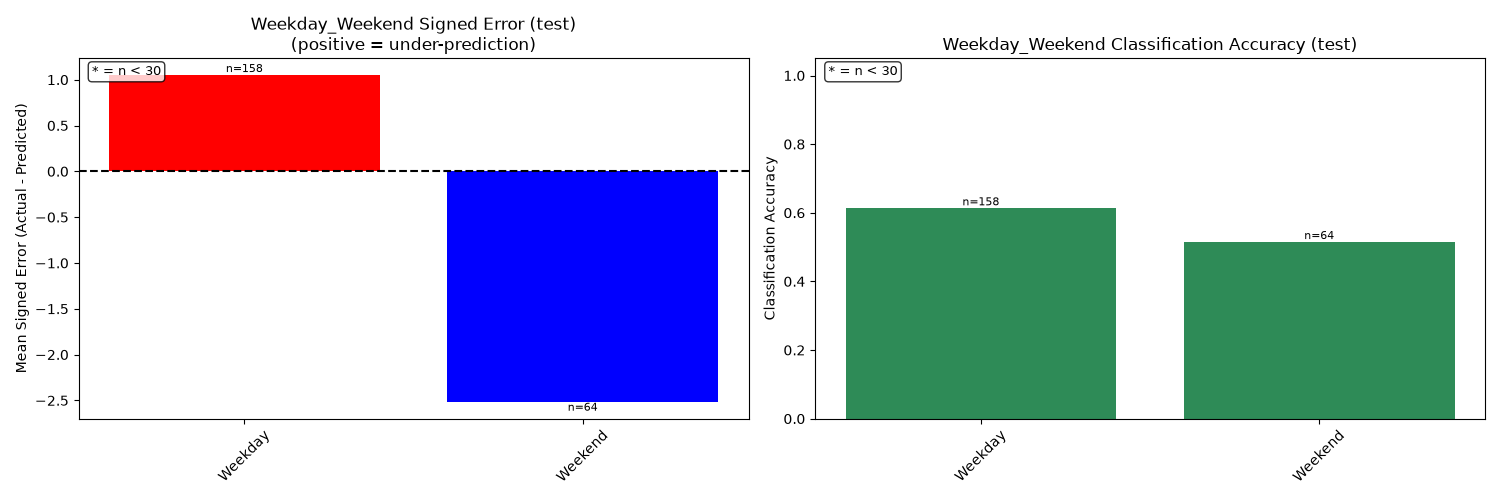
\includegraphics[width=0.95\linewidth]{bias_Weekday_Weekend_test.png}
  \caption{Test signed error and classification accuracy for weekday versus weekend rows.}
  \label{fig:bias-weekday}
\end{figure}

\begin{figure}[htbp]
  \centering
  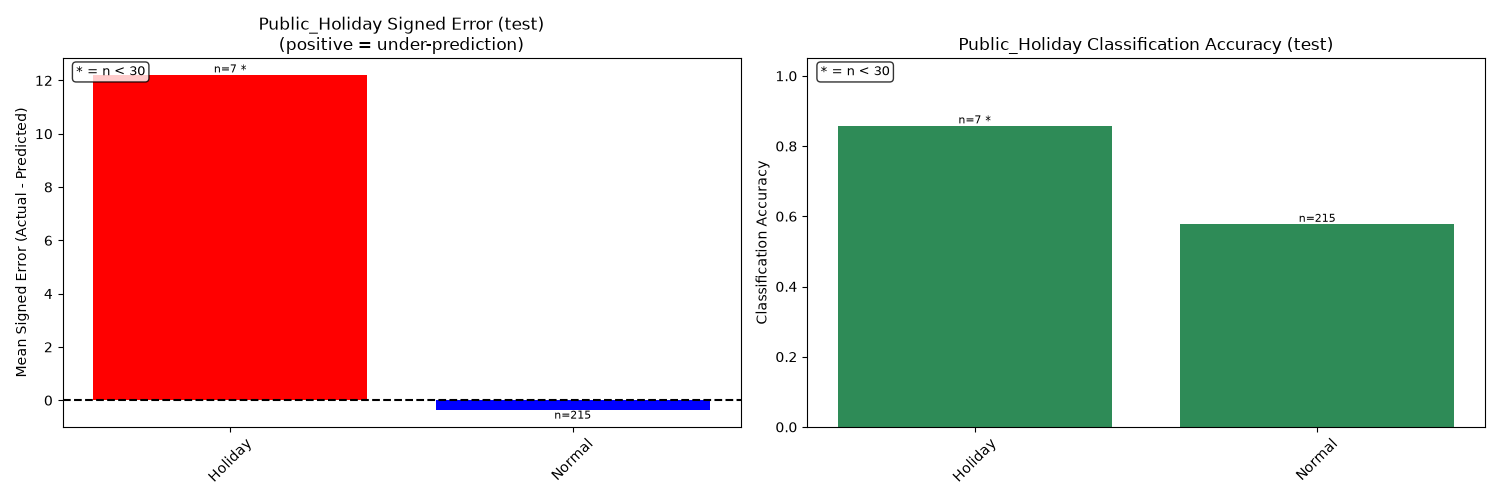
\includegraphics[width=0.95\linewidth]{bias_Public_Holiday_test.png}
  \caption{Test signed error and classification accuracy for normal days versus public holidays. Holiday support is only seven rows.}
  \label{fig:bias-holiday}
\end{figure}

The full set of 14 bias charts (seven dimensions for validation and test) is included in the \texttt{figures/} folder. The charts mark groups with $n<30$ with an asterisk; those estimates should not be read as precise.

The class mix also shifts across periods. Unhealthy is about 48\% of training rows but 32\% of validation and 35\% of test. The two Hazardous bands together are about 10\% of training but 22\% of validation and 19\% of test. This may reflect seasonal composition, missing training days or targets, or real worsening; the data do not identify a single cause. The later-period under-prediction of severe days is consistent with that shift, but it is not proof of a causal trend.

\section{Phase 4: Model limitations and recommendations}

\begin{itemize}[leftmargin=1.4em]
  \item \textbf{Rare-class uncertainty.} Good/Moderate has 8 test rows and Hazardous 401--500 has 19. Their per-class precision/recall are noisy. The same applies to small bias subgroups such as public holidays and the 500+ severity band.
  \item \textbf{Single station.} The dataset represents one monitoring location and has no demographic attributes. The bias check cannot support claims about population-level fairness.
  \item \textbf{Distribution shift.} The class mix and the validation-to-test error pattern change over time. A model selected on validation can fail to beat persistence on a later period, as happened on both tasks (macro F1 below persistence for classification, and essentially tied on RMSE for regression).
  \item \textbf{Coverage gaps.} The validation split contains 250 usable rows over the 326 days from 2023-07-14 to 2024-06-03 (about 77\%), because many days lack an AQI label or a next-day target; the test split has 223 rows over the 224 days from 2024-07-08 to 2025-02-16 and contains no spring rows. Validation and test therefore cover different seasonal mixes, which limits how directly their metrics can be compared.
  \item \textbf{Macro F1 versus accuracy.} HGB's test accuracy is higher than persistence's, but its macro F1 is lower. Reporting only accuracy would obscure the rare-class weakness.
  \item \textbf{No traffic data.} Calendar features are proxies; no open, time-aligned Lahore traffic dataset was available. This limits the explanatory scope of the features.
  \item \textbf{No test-time retuning.} The report preserves the validation-based selection. Switching to Ridge after seeing test would be post-hoc and would invalidate the test-once rule.
\end{itemize}

Recommended next steps are to collect more severe-pollution days, evaluate cost-sensitive or class-balanced variants with a pre-registered validation rule, add calibrated probabilities and prediction intervals, and test on a later period or a second station. Any such change should be selected without using the current test set.

\section{Phase 4: Reproducibility}

The final results were produced from merge commit \texttt{a55a7f5} on \texttt{main}; the repository README was updated afterwards (commit \texttt{56dea73}). The final pipeline was run from the repository root with:

\begin{verbatim}
python -m src.check_setup
python -m unittest discover -s tests -t .
python -m src.classification
python -m src.regression
python -m src.bias_analysis
\end{verbatim}

\texttt{check\_setup} reported 0 bad next-day PM2.5 values, 0 bad lag-1 values, and 0 bad next-day categories. The unit tests ran 15 tests and passed. Classification completed in 427.92 seconds and regression in 37.61 seconds. The bias analysis then joined the final prediction files.

The classification prediction file has 473 rows and 12 columns; 466 rows are scorable. Its SHA-256 hash is \texttt{47D8E0A89FC3F37EA6B74E807DCF566FBDD6D79F734D5A05CFD56124888EB2EB}, matching the verified Drive copy. Regression also has 473 prediction rows, 466 scorable.

Dependencies are listed in \texttt{requirements.txt}. The final environment used pandas 3.0.3, scikit-learn 1.9.1, and matplotlib 3.11.2. The seed is 42 from \texttt{configs/base.yaml}. Generated prediction CSVs, metrics JSON, and charts are review artifacts and should not be committed to Git; the data and large artifacts belong on the shared Drive or a release link. No fitted model weights are published: the selected pipelines are refit from fixed seeds by the committed scripts (see the repository README).

\subsection{Git-author contributions}

Table~\ref{tab:git-authors} is the Git-author contribution table: it maps each commit author to the project modules and representative commits they own. The repository history contains only the three project contributors. The Git identities used in the D2 work are Abdul Rehman \texttt{<}\url{arehman4275@gmail.com}\texttt{>}, Muhammad Haider Mughal \texttt{<}\url{haiderirfanmm@gmail.com}\texttt{>}, and Muhammad Ayub Butt \texttt{<}\url{purestudy83010@gmail.com}\texttt{>}. Some earlier commits by the same author also appear under the display name ``Haider Mughal'' with the same e-mail address. No AI or OpenCode co-author trailer was added.

\begin{table}[htbp]
\centering
\footnotesize
\caption{Git-author contribution table: commit authors mapped to project modules. The package and report list exactly the three human project contributors.}
\label{tab:git-authors}
\begin{tabular}{llL{4.5cm}L{4.9cm}}
\toprule
Contributor & ID & D2 contribution & Key modules and representative commits \\
\midrule
Abdul Rehman & 3059 & Shared data and evaluation foundation; integration; D2 report & \texttt{src/data.py}; \texttt{src/evaluate.py}; \texttt{src/check\_setup.py}; \texttt{configs/base.yaml}; \texttt{tests/test\_evaluate.py}; \texttt{reports/} (\texttt{b672bfc}, \texttt{20fa79e}, \texttt{a55a7f5}) \\
Muhammad Haider Mughal & 3006 & Classification pipeline and tuning & \texttt{src/classification.py} (\texttt{d311f8e}, \texttt{5f57987}) \\
Muhammad Ayub Butt & 3076 & Regression and bias analysis & \texttt{src/regression.py}; \texttt{src/bias\_analysis.py} (\texttt{fae7490}, \texttt{6e2448d}) \\
\bottomrule
\end{tabular}
\end{table}


\section{Phase 4: Evaluation summary}

The primary classification model, HGB, was selected on validation macro F1 and reached 0.4780 on test. It did not beat persistence's 0.5157 macro F1, even though its accuracy was slightly higher. The secondary regression model, HGB, was selected on validation RMSE only; test results were not used to change the selection. Its test RMSE was 64.9198, essentially tied with persistence's 64.8175 (a 0.10 gap and skill $-0.0016$). Ridge did beat persistence on test with RMSE 62.0956, but switching to it after seeing test would violate the validation-only selection rule. The bias analysis shows that the largest error magnitudes occur on the most severe pollution days; because those groups are defined by the observed outcome, the sign is partly constructed, so the magnitude is the informative result. Seasonal and temporal errors are also uneven. These results are reported as observed, without retuning on the test set.

% Phase 5 and Phase 6: the Deliverable 3 application, explainability,
% final evaluation, and discussion. Included by report_d3.tex.

\section{Phase 5: Application and Explainability}
\label{sec:phase5}

Deliverable 3 (Track A) turns the frozen Deliverable 2 pipelines into a
working, explainable application. It does not retrain, retune, or reselect a
model. The regression and classification pipelines, their preprocessing, the
chronological split, and the reported test scores are exactly those of
Deliverable 2. The new contribution is the application and inference layer:
a six-input forecast screen, an 80\% prediction interval, local and global
explanations, historical seasonal context, a persistence comparison, and a
reproducible artifact pipeline.

This distinction matters for the evaluation. The application cannot repair a
model that ties or loses to persistence. It can, however, make the forecast
usable, show its uncertainty, expose its limitations, and prevent the user from
mistaking a demonstration for an operational warning system.

\subsection{Design goals and scope}
\label{sec:d3-goals}

Table~\ref{tab:d3-goals} maps the Track A requirements to the implementation and
to the evidence that the requirement was met. The design goals were deliberately
narrow: a working local application, transparent behaviour, and an honest
comparison with the simplest baseline.

\begin{table}[htbp]
\centering
\footnotesize
\begin{tabular}{@{}L{3.7cm}L{7.0cm}L{4.6cm}@{}}
\toprule
\textbf{Design goal} & \textbf{Implementation} & \textbf{Evidence} \\
\midrule
Next-day PM$_{2.5}$ and AQI forecast &
Frozen HGB regression and six-class HGB classifier in
\texttt{src/inference.py}; the app shows both views &
Regression test RMSE 64.92; classifier test macro-F1 0.478 \\
Uncertainty &
Quantile HGB models at the 10th and 90th percentiles, with a
validation-calibrated 80\% central interval &
Validation coverage 80.3\%; test coverage 77.0\% \\
Explanations &
One-at-a-time local sensitivity and validation-set permutation
importance &
Sensitivity chart and top-feature panel in the app \\
Historical context &
Monthly medians, winter stagnation, seasonal means, and an
hourly profile &
Metadata generated by \texttt{src/train\_pipeline.py} and
\texttt{src/hourly.py} \\
Honest baseline comparison &
Persistence is displayed on every forecast; the app warns when
the two category views disagree &
Test metrics and the persistence card are shown in the result
panel \\
Reproducibility &
Frozen hyperparameters, fixed seed, refit script, 14 tests, and
no committed binaries &
The D3 refit reproduces the D2 metrics exactly \\
Documentation &
\texttt{README.md}, \texttt{STUDY\_REPORT.md}, this report, and
the report build script &
The repository is self-contained apart from the external data
files \\
\bottomrule
\end{tabular}
\caption{Deliverable 3 design goals and evidence. The model itself is unchanged
from Deliverable 2.}
\label{tab:d3-goals}
\end{table}

\paragraph{Scope.} The application is an \emph{illustrative single-day
forecaster}, not a live feed. The user supplies six values for today; the app
returns a forecast for the following day. It does not ingest a live weather
feed, a live sensor stream, or a multi-day history. The remaining model inputs
use training-set medians or modes, and the PM$_{2.5}$ lags and rolling windows
are held at today's value. Section~\ref{sec:d3-features} explains why this is a
deliberate usability trade-off and where it can mislead.

\subsection{System architecture and artifact policy}
\label{sec:d3-architecture}

Figure~\ref{fig:d3-architecture} shows the six layers of the delivered system.
The committed data layer contains the source scripts and documentation; the
processed feature table is derived and is not committed. The model layer refits
the frozen pipelines and writes four joblib artifacts plus a metadata file. The
pipelines use scikit-learn's histogram gradient boosting~\cite{scikit,hgb}. The
application layer loads those artifacts and performs feature assembly,
prediction, interval construction, explanations, and guidance. The interface
layer is the Streamlit screen~\cite{streamlit}. The evaluation layer contains the ablation and
the unit tests. The user outputs are the forecast cards, interval, guidance,
and charts.

\begin{figure}[htbp]
  \centering
  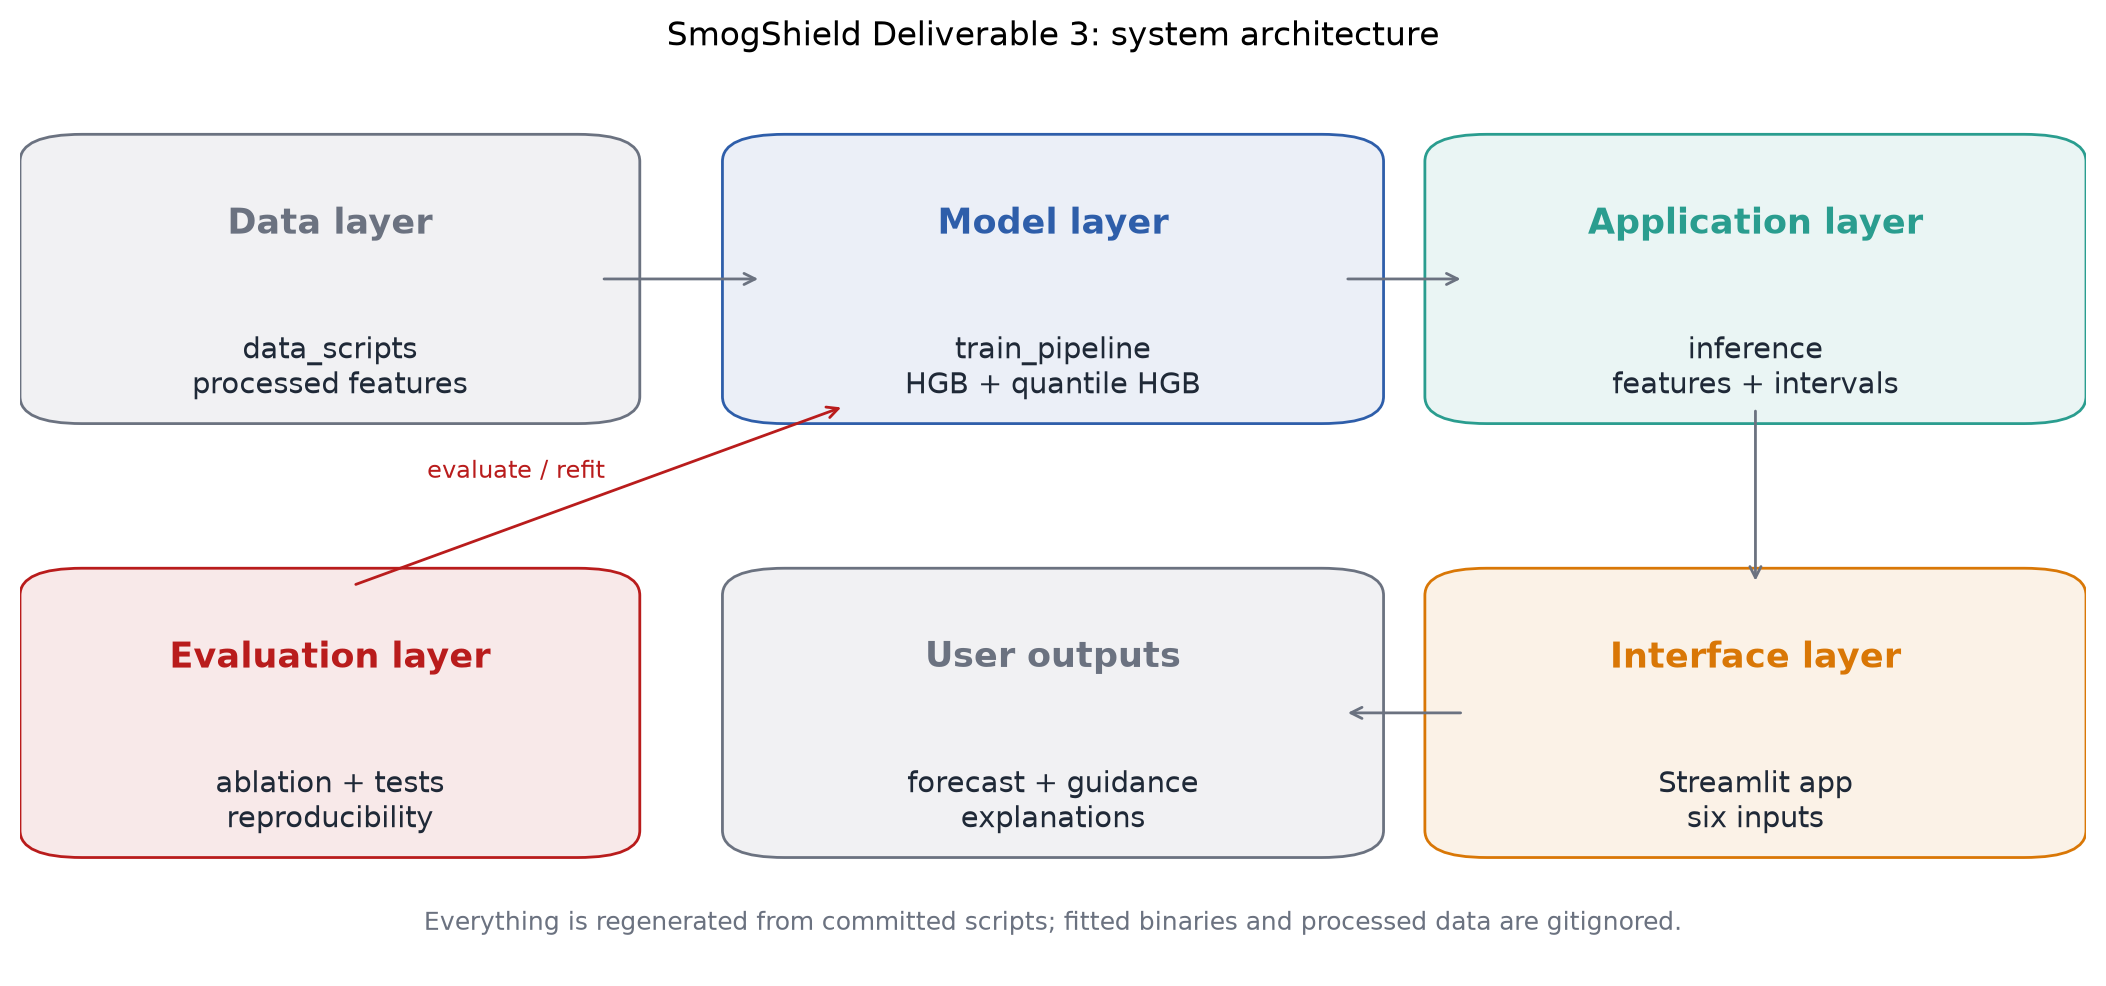
\includegraphics[width=\linewidth]{fig_architecture.png}
  \caption{Deliverable 3 system architecture. Fitted artifacts and processed
  data are regenerated from committed scripts; they are not committed to Git.}
  \label{fig:d3-architecture}
\end{figure}

Table~\ref{tab:artifacts} lists the runtime artifacts. The important policy is
that no fitted model binary and no processed data file is committed. The
repository contains the scripts that recreate them from fixed seeds. This is the
same policy used in Deliverable 2, extended to the four new pipelines and the
metadata file.

\begin{table}[htbp]
\centering
\footnotesize
\begin{tabular}{@{}L{5.4cm}L{3.5cm}L{3.5cm}L{2.6cm}@{}}
\toprule
\textbf{Artifact} & \textbf{Produced by} & \textbf{Consumed by} & \textbf{Committed?} \\
\midrule
\path{models/regression_pipeline.joblib} &
\texttt{src/train\_pipeline.py} & \texttt{src/inference.py} & No \\
\path{models/regression_q10_pipeline.joblib} &
\texttt{src/train\_pipeline.py} & \texttt{src/inference.py} & No \\
\path{models/regression_q90_pipeline.joblib} &
\texttt{src/train\_pipeline.py} & \texttt{src/inference.py} & No \\
\path{models/classification_pipeline.joblib} &
\texttt{src/train\_pipeline.py} & \texttt{src/inference.py} & No \\
\texttt{models/metadata.json} &
\texttt{src/train\_pipeline.py} & \texttt{src/inference.py}, app & No \\
\texttt{models/ablation.json} &
\texttt{src/ablation.py} & report, review & No \\
\path{data/processed/features_daily.csv} &
\path{data_scripts/09_build_features.py} &
\texttt{src/train\_pipeline.py} & No \\
\path{data/processed/pm25_hourly.csv} &
\path{data_scripts/02_clean_pm25_simple.py} &
\texttt{src/hourly.py} & No \\
\bottomrule
\end{tabular}
\caption{Runtime artifacts and their Git policy. The model directory has its own
\texttt{.gitignore}; the processed data directory is ignored at the repository
root.}
\label{tab:artifacts}
\end{table}

The architecture separates \emph{training} from \emph{serving}. The Streamlit
app imports \texttt{src.inference}, not the training modules. The inference
module loads the pipelines once, caches them in memory, and exposes a single
\texttt{predict()} call. If the artifacts are missing, it raises an error that
points the user at \texttt{python -m src.train\_pipeline}. This makes the failure
mode explicit rather than silently serving a stale or partial model.

\subsection{From six inputs to 46 features}
\label{sec:d3-features}

The model contract contains 46 raw features, which become 80 encoded columns
after one-hot encoding and missing-value indicators. The app collects only six
user-facing inputs. Table~\ref{tab:app-inputs} shows how each input is mapped
onto the model's real feature names.

\begin{table}[htbp]
\centering
\footnotesize
\begin{tabular}{@{}L{2.3cm}L{2.1cm}L{5.6cm}L{5.2cm}@{}}
\toprule
\textbf{App input} & \textbf{Unit} & \textbf{Derived model features} & \textbf{Default} \\
\midrule
Feature date & date &
\texttt{month}, \texttt{day\_of\_year}, \texttt{weekday},
\texttt{is\_weekend}, sin/cos terms, season dummies &
Today's date \\
Today's PM$_{2.5}$ & $\mu$g/m$^3$ &
\texttt{pm25}, \texttt{pm25\_log}, numeric \texttt{aqi}, lags 1--3,
rolling 3/7, difference &
Monthly historical median \\
Today's AQI category & seven raw labels &
\texttt{aqi\_category} (one-hot encoded) &
Derived from the default PM$_{2.5}$ \\
Temperature & $^\circ$C &
\texttt{temp\_mean\_c}, \texttt{temp\_max\_c}, \texttt{temp\_min\_c},
\texttt{temp\_mean\_c\_lag1} & 22 \\
Relative humidity & \% &
\texttt{humidity\_mean\_pct}, \texttt{humidity\_mean\_pct\_lag1} & 60 \\
Wind speed & km/h &
\texttt{wind\_speed\_mean\_kmh}, \texttt{wind\_speed\_max\_kmh},
\texttt{wind\_speed\_mean\_kmh\_lag1} & 7 \\
\bottomrule
\end{tabular}
\caption{The six user inputs and the model features they populate. Unlisted
features use training-set medians or modes.}
\label{tab:app-inputs}
\end{table}

The feature contract is filled in four steps. First, \texttt{build\_feature\_row}
starts from the training medians for numeric features and the training modes for
categorical features, both stored in \texttt{metadata.json}. Second, it maps the
six friendly inputs onto the model columns. Third, it derives the PM$_{2.5}$
history as a steady state: lags 1--3, the 3-day and 7-day rolling means, and the
day-to-day difference are set from today's PM$_{2.5}$, with the difference set to
zero. Fourth, explicit feature-column overrides are applied last. The
date-derived calendar features are computed from the selected feature date, not
from the forecast date; the forecast is always for the following day.

\paragraph{The numeric AQI fix.} The app does not ask for a numeric AQI. In an
early version the \texttt{aqi} feature therefore stayed at the training median of
165 even when the user entered a clean or hazardous PM$_{2.5}$ value. That was
internally inconsistent: the model saw a category and a PM$_{2.5}$ value that did
not correspond to the same AQI. The inference layer now derives \texttt{aqi} from
the entered PM$_{2.5}$ through the same US-EPA breakpoints used to build the
training labels. This is an inference-layer fix; the fitted pipelines and all
reported metrics are unchanged.

\paragraph{The category input is nearly inert.} The raw AQI category is a
categorical feature, but the numeric AQI and PM$_{2.5}$ carry almost all of the
signal. In an audit of the default November example, changing the category input
across all seven raw labels left the regression prediction identical to two
decimals (189.74 $\mu$g/m$^3$). The classifier's top probability moved only
between 0.9865 and 0.9910, and its arg-max stayed \emph{Very Unhealthy}. This is
not a bug in the UI; it is a property of the fitted model. The app keeps the
category input because it is part of the model contract and because the raw
seven-label vocabulary is familiar to users, but the report does not claim that
the category selector drives the forecast.

\begin{table}[htbp]
\centering
\small
\begin{tabular}{@{}lrr@{}}
\toprule
\textbf{Input category} & \textbf{Regression PM$_{2.5}$} &
\textbf{Classifier top label (probability)} \\
\midrule
Good & 189.74 & Very Unhealthy (0.991) \\
Moderate & 189.74 & Very Unhealthy (0.991) \\
Unhealthy for Sensitive & 189.74 & Very Unhealthy (0.991) \\
Unhealthy & 189.74 & Very Unhealthy (0.987) \\
Very Unhealthy & 189.74 & Very Unhealthy (0.991) \\
Hazardous (301--400) & 189.74 & Very Unhealthy (0.991) \\
Hazardous (401--500) & 189.74 & Very Unhealthy (0.991) \\
\bottomrule
\end{tabular}
\caption{Category-input audit for the default November example (PM$_{2.5}$ =
234.2, temperature 22$^\circ$C, humidity 60\%, wind 7 km/h, 12 November 2026).
The numeric PM$_{2.5}$ and derived AQI dominate; the category selector is nearly
inert.}
\label{tab:category-audit}
\end{table}

\paragraph{Feature groups.} Table~\ref{tab:feature-groups} groups the 46 raw
features. The 12 history features are the inputs that the ablation calls
``history only.'' Adding 17 calendar features gives the 29-feature set; adding
17 weather features gives the full 46-feature set. This is the same nested
design used in the Deliverable 3 ablation.

\begin{table}[htbp]
\centering
\small
\begin{tabular}{@{}L{3.4cm}rL{9.2cm}@{}}
\toprule
\textbf{Feature group} & \textbf{Raw count} & \textbf{Examples} \\
\midrule
Air quality and history & 12 &
\texttt{pm25}, \texttt{aqi}, \texttt{aqi\_category}, \texttt{pm25\_log},
lags 1--3, rolling 3/7, difference, data-quality flags \\
Calendar and events & 17 &
month, day-of-year, weekday, weekend, sin/cos terms, season dummies,
Ramadan, Eid, public holiday \\
Weather & 17 &
temperature (mean/max/min/lag), humidity (mean/lag), dew point, pressure
(mean/lag), wind (mean/max/lag/direction), rain, solar radiation, cloud cover \\
\midrule
Total & 46 & 80 encoded columns after preprocessing \\
\bottomrule
\end{tabular}
\caption{The nested feature groups. The ablation uses the 12-, 29-, and
46-feature sets with the same frozen hyperparameters.}
\label{tab:feature-groups}
\end{table}

\subsection{The forecast screen}
\label{sec:d3-ui}

Figure~\ref{fig:d3-ui} shows the flow of the forecast screen. The user enters
the six values in a two-column form. Pressing \emph{Forecast next day} calls
\texttt{inference.predict()} and returns three rows of output. The first row
shows the predicted PM$_{2.5}$, the AQI implied by that PM$_{2.5}$, and the
implied AQI category. The second row shows the classifier's category, its
confidence, and the persistence value. The third block shows the 80\% interval,
the guidance banner, the local sensitivity chart, and the expanders for global
importance, winter stagnation, and the hourly profile.

\begin{figure}[htbp]
  \centering
  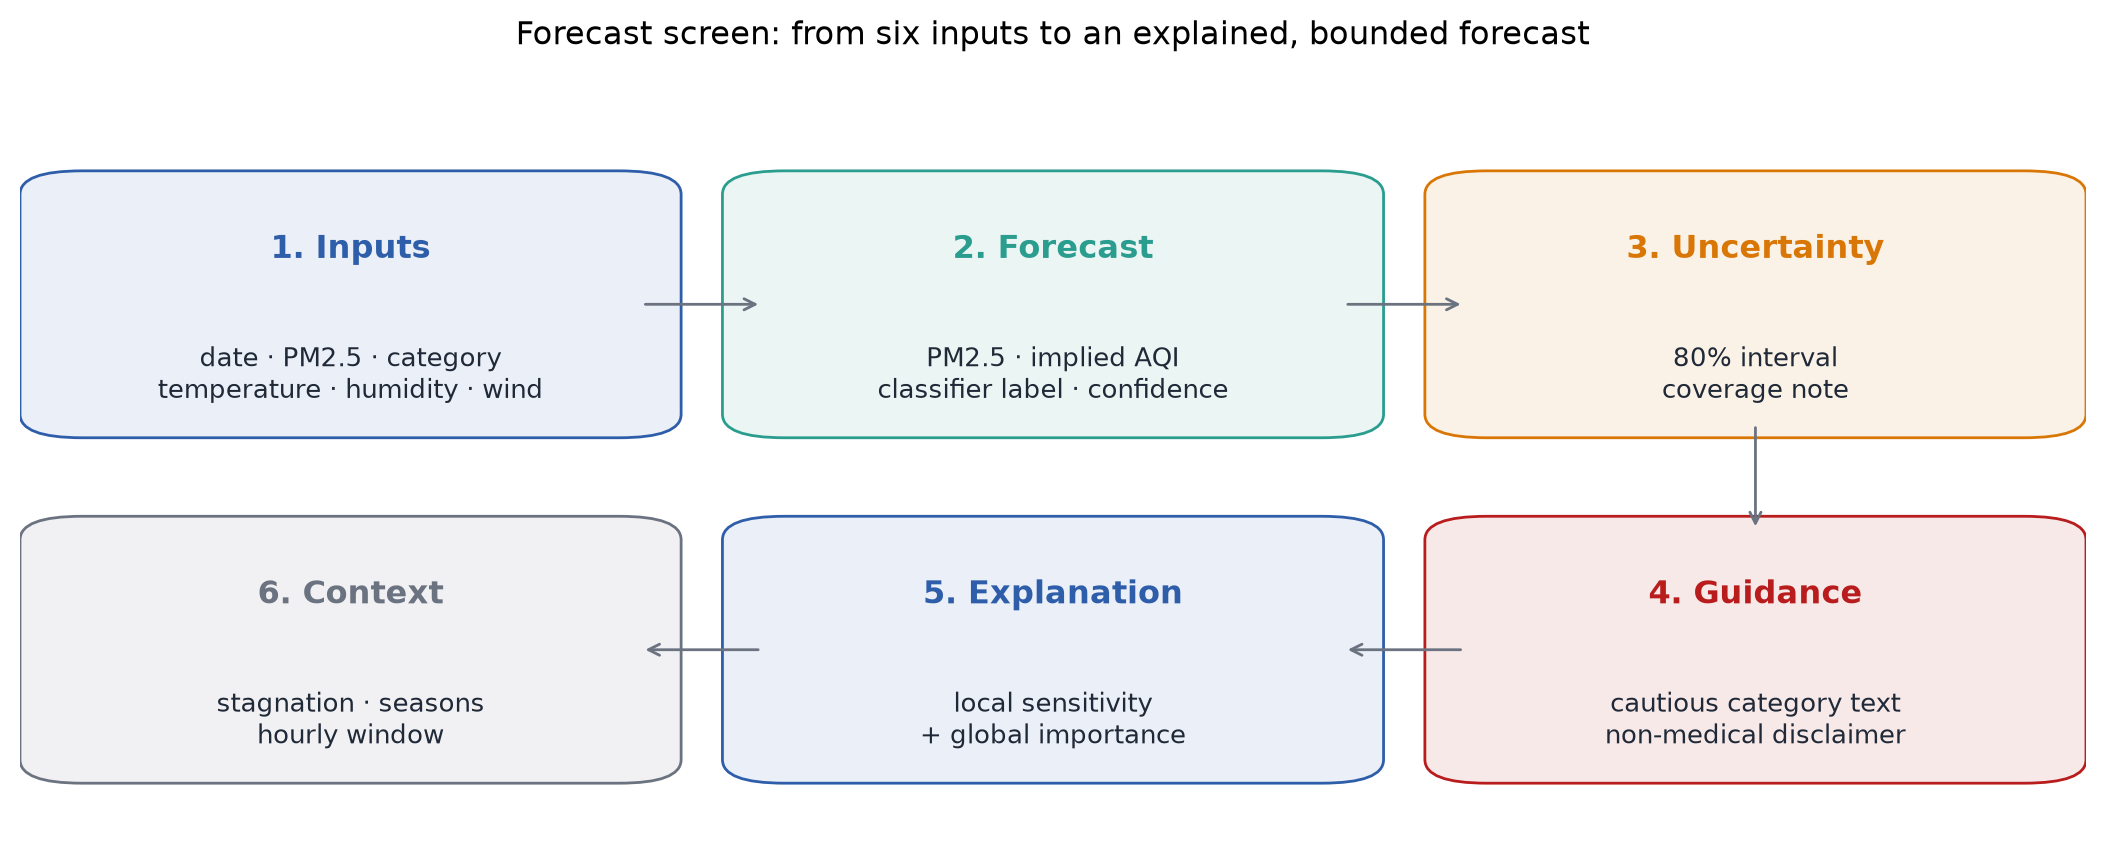
\includegraphics[width=\linewidth]{fig_ui_flow.png}
  \caption{The forecast screen in six steps. The interface is a single
  Streamlit page; the expanders keep the historical context available without
  crowding the primary forecast.}
  \label{fig:d3-ui}
\end{figure}

Table~\ref{tab:ui-outputs} explains each output. The table is intentionally
redundant with the app: a user should not have to infer what a card means, and a
reviewer should be able to check that the screen is not hiding a weaker result.

\begin{table}[htbp]
\centering
\footnotesize
\begin{tabular}{@{}L{3.1cm}L{6.1cm}L{5.9cm}@{}}
\toprule
\textbf{Output} & \textbf{What it shows} & \textbf{How to read it} \\
\midrule
Predicted PM$_{2.5}$ & Regression point forecast for tomorrow &
A single number in $\mu$g/m$^3$; not a guarantee \\
AQI implied by PM$_{2.5}$ & US-EPA AQI computed from the predicted PM$_{2.5}$ &
Monotonic in the prediction; uses the same breakpoints as the labels \\
Implied category & EPA category of the implied AQI &
The more defensible category view because the classifier was weaker than
persistence \\
Classifier category and confidence & Six-class HGB arg-max and its probability &
A separate model; biased toward \emph{Unhealthy} \\
Persistence & Tomorrow = today, for PM$_{2.5}$ and category &
The baseline the model must beat; shown on every forecast \\
80\% interval & Calibrated central interval for next-day PM$_{2.5}$ &
A range, not a worst case; test coverage is 77.0\% \\
Local sensitivity & Change in the forecast when one input is increased &
A finite difference, not a causal effect \\
Global importance & Permutation importance on validation &
Which features the model relies on overall \\
Winter stagnation & Share of stagnant winter days and their mean PM$_{2.5}$ &
Descriptive history, not a today-specific forecast \\
Best time outdoors & Hour-of-day and seasonal PM$_{2.5}$ profile &
Station-specific history; winter afternoons remain polluted \\
Guidance & Cautious, non-medical advice for the implied category &
Follow official advisories; not medical advice \\
Disagreement warning & Appears when the two category views differ &
Explains which view the app recommends and why \\
\bottomrule
\end{tabular}
\caption{The forecast screen outputs and their interpretation.}
\label{tab:ui-outputs}
\end{table}

The interface was exercised with Streamlit's application test harness. The
AppTest run reported no exceptions, four charts, and three expanders. This is a
smoke test, not a usability study: it confirms that the page renders and the
main branches execute, not that the wording is clear to a first-time user.

\subsection{Prediction intervals}
\label{sec:d3-intervals}

A point forecast is not enough for a decision. The app therefore trains two
additional HGB models with quantile loss, one at the 10th percentile and one at
the 90th percentile, and combines them into an 80\% central prediction interval.
The bounds are forced to contain the point forecast and are then widened by a
calibration factor chosen on the validation split. On this dataset the factor is
1.00, so no widening was needed. Validation coverage is 80.3\%; test coverage is
77.0\%. The test split is used only to report coverage, never to choose the
factor.

\begin{table}[htbp]
\centering
\small
\begin{tabular}{@{}lr@{}}
\toprule
\textbf{Property} & \textbf{Value} \\
\midrule
Nominal level & 80\% \\
Quantiles & 10th and 90th \\
Calibration scale & 1.00 \\
Validation coverage & 80.3\% \\
Test coverage & 77.0\% \\
Tuning rule & Validation only; test reported, never tuned \\
\bottomrule
\end{tabular}
\caption{The 80\% prediction interval. The test coverage is below nominal, which
is reported rather than hidden.}
\label{tab:interval}
\end{table}

Figure~\ref{fig:d3-interval} shows the nominal-versus-empirical coverage and the
default November example. The default is deliberately a polluted day: today's
PM$_{2.5}$ is the historical November median, 234.2 $\mu$g/m$^3$; the app
forecasts 189.74 $\mu$g/m$^3$ with an interval of 133.8--294.1 $\mu$g/m$^3$.
The interval spans categories from \emph{Unhealthy} to \emph{Hazardous
(301--400)}, even though the point forecast is \emph{Very Unhealthy}. That width
is the honest message: the model is not precise enough to support a single
category claim.

\begin{figure}[htbp]
  \centering
  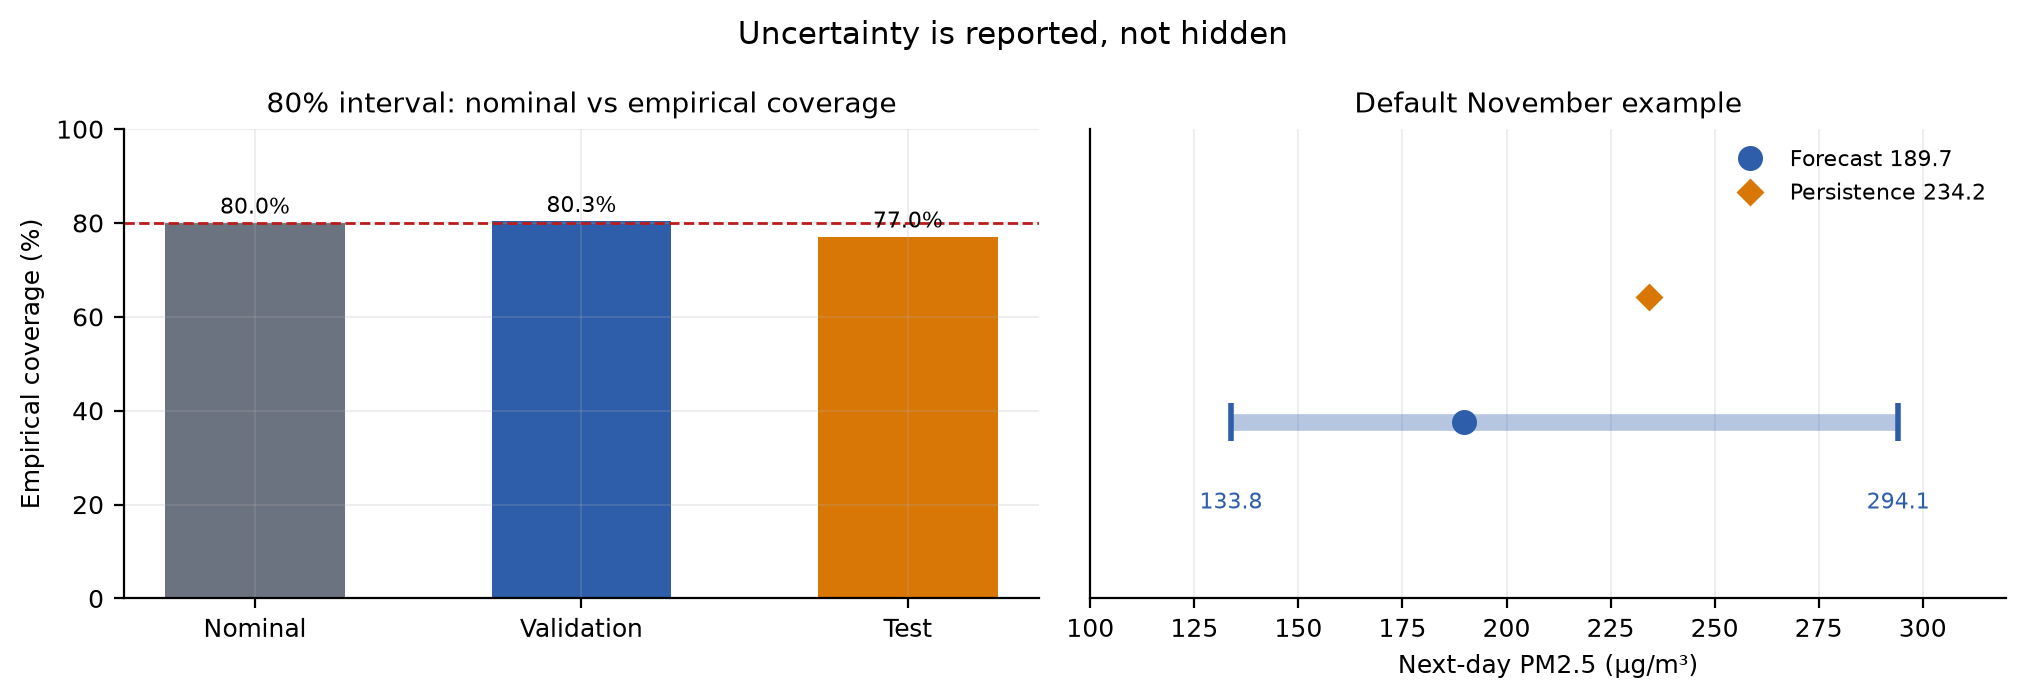
\includegraphics[width=\linewidth]{fig_interval.png}
  \caption{Left: nominal 80\% coverage versus validation and test coverage.
  Right: the default November forecast and its 80\% interval, compared with
  persistence. The interval is wide because the model is uncertain, not because
  the app is hiding a point estimate.}
  \label{fig:d3-interval}
\end{figure}

The interval is a central interval for the \emph{next-day PM$_{2.5}$ observation},
not a confidence interval for the model's mean prediction. It does not include
model-selection uncertainty, distribution shift, or the error introduced by the
steady-state feature assumption. A future version should add conformal
prediction and a separate interval for the AQI category.

\subsection{Explanations: global and local}
\label{sec:d3-explanations}

The app provides two explanations with different scopes. The global explanation
uses permutation importance on the validation split: one feature at a time is
shuffled, and the increase in RMSE (regression) or the drop in macro-F1
(classification) is recorded. The local explanation perturbs one input for the
current forecast and reports the change in the predicted PM$_{2.5}$.

\paragraph{Global view.} Figure~\ref{fig:d3-importance} and
Table~\ref{tab:importance} show the top features. For regression, today's
PM$_{2.5}$ is dominant (increase in RMSE 14.51), followed by the numeric AQI
(4.20), day-of-year (4.15), lag-1 PM$_{2.5}$ (2.93), and wind direction (2.50).
For classification, the top features are PM$_{2.5}$ (drop in macro-F1 0.0786),
wind direction (0.0672), pressure (0.0506), numeric AQI (0.0495), and the
day-of-year cosine (0.0407). The presence of day-of-year and seasonal terms is
consistent with the strong winter cycle.

The ranking is descriptive, not causal. Permutation importance breaks the
relationship between a feature and its correlated neighbours. Shuffling
\texttt{pm25} while leaving the lags intact can overstate its unique
contribution; conversely, a feature that is redundant with another may look
unimportant. The report uses the ranking to explain what the model relies on,
not to claim that changing a feature would change the outcome by that amount.

\begin{figure}[htbp]
  \centering
  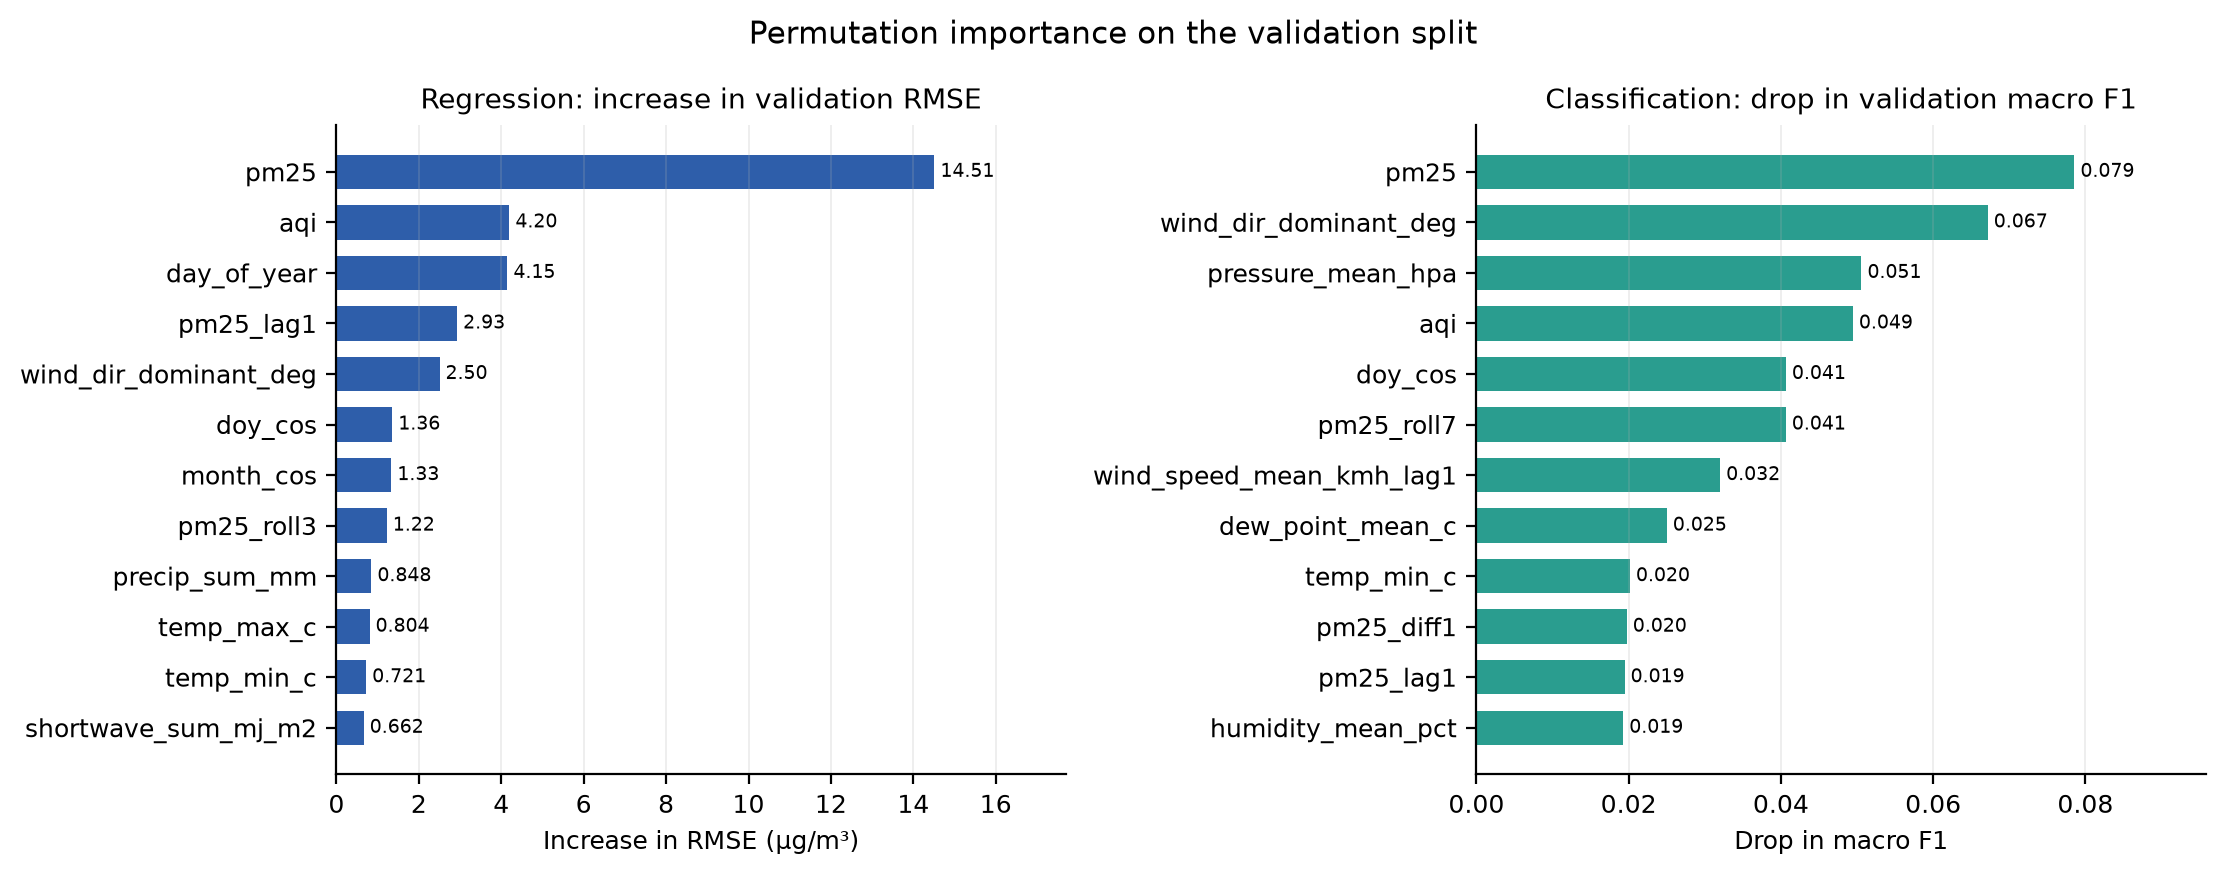
\includegraphics[width=\linewidth]{fig_importance.png}
  \caption{Permutation importance on the validation split. Regression scores are
  the increase in RMSE when a feature is shuffled; classification scores are the
  drop in macro-F1. Correlated features share credit, so the ranking is not a
  causal decomposition.}
  \label{fig:d3-importance}
\end{figure}

\begin{table}[htbp]
\centering
\footnotesize
\begin{tabular}{@{}rlrrl r@{}}
\toprule
\multicolumn{3}{c}{\textbf{Regression (increase in RMSE)}} &
\multicolumn{3}{c}{\textbf{Classification (drop in macro-F1)}} \\
\cmidrule(lr){1-3}\cmidrule(lr){4-6}
\textbf{Rank} & \textbf{Feature} & \textbf{Value} &
\textbf{Rank} & \textbf{Feature} & \textbf{Value} \\
\midrule
1 & \texttt{pm25} & 14.51 & 1 & \texttt{pm25} & 0.0786 \\
2 & \texttt{aqi} & 4.20 & 2 & \texttt{wind\_dir\_dominant\_deg} & 0.0672 \\
3 & \texttt{day\_of\_year} & 4.15 & 3 & \texttt{pressure\_mean\_hpa} & 0.0506 \\
4 & \texttt{pm25\_lag1} & 2.93 & 4 & \texttt{aqi} & 0.0495 \\
5 & \texttt{wind\_dir\_dominant\_deg} & 2.50 & 5 & \texttt{doy\_cos} & 0.0407 \\
6 & \texttt{doy\_cos} & 1.36 & 6 & \texttt{pm25\_roll7} & 0.0406 \\
7 & \texttt{month\_cos} & 1.33 & 7 & \texttt{wind\_speed\_mean\_kmh\_lag1} & 0.0320 \\
8 & \texttt{pm25\_roll3} & 1.22 & 8 & \texttt{dew\_point\_mean\_c} & 0.0250 \\
\bottomrule
\end{tabular}
\caption{Top eight permutation-importance features for the two tasks.}
\label{tab:importance}
\end{table}

\paragraph{Local view.} The local explanation answers a narrower question: for
\emph{this} forecast, what happens if one input is increased by a fixed amount?
The app perturbs four inputs: PM$_{2.5}$ by +25 $\mu$g/m$^3$, temperature by
+5$^\circ$C, humidity by +10 percentage points, and wind speed by +5 km/h. The
PM$_{2.5}$ step is larger than the others because HGB predictions are piecewise
constant: a +10 step often stays inside the same leaf and reports a misleading
0.0. A +25 step crosses splits more reliably, but it is still a finite
difference, not a smooth slope.

Table~\ref{tab:local} shows the local explanation for the default November
example. A +25 $\mu$g/m$^3$ increase in today's PM$_{2.5}$ raises the forecast by
38.68 $\mu$g/m$^3$; a +5$^\circ$C temperature increase raises it by 18.41; a
+5 km/h wind increase lowers it by 7.08; and a +10-point humidity increase
lowers it by 0.43. The wind sign matches the physical intuition that stronger
wind disperses pollution. The temperature sign is local and counter-intuitive
at first glance; it should not be read as a causal effect, because temperature
is correlated with season, pressure, and the winter inversion regime.

\begin{table}[htbp]
\centering
\small
\begin{tabular}{@{}lrr@{}}
\toprule
\textbf{Input change} & \textbf{Change in forecast} & \textbf{Direction} \\
\midrule
PM$_{2.5}$ +25 $\mu$g/m$^3$ & +38.68 & Higher forecast \\
Temperature +5$^\circ$C & +18.41 & Higher forecast \\
Wind +5 km/h & $-7.08$ & Lower forecast \\
Humidity +10 points & $-0.43$ & Slightly lower forecast \\
\bottomrule
\end{tabular}
\caption{Local sensitivity for the default November example (point forecast
189.74 $\mu$g/m$^3$). The values are one-at-a-time finite differences, not
causal effects.}
\label{tab:local}
\end{table}

The app ranks the four bars by absolute effect. A zero-length bar is possible
even for an important feature if the perturbation stays inside a leaf; the
larger PM$_{2.5}$ step reduces, but does not eliminate, that artifact. A
Shapley-value decomposition would be a more principled local explanation and is
left as future work.

\subsection{Seasonal defaults and historical context}
\label{sec:d3-seasonal}

The app opens on a seasonally plausible scenario rather than a fixed clean-day
value. The initial PM$_{2.5}$ is the historical median for the current calendar
month, and the initial category is derived from that PM$_{2.5}$ through the EPA
breakpoints. On 12 November 2026 the default is 234.2 $\mu$g/m$^3$ and
\emph{Very Unhealthy}; the forecast is 189.74 $\mu$g/m$^3$, still
\emph{Very Unhealthy}, with a persistence value of 234.2 $\mu$g/m$^3$.

This choice matters for the demo. A fixed 60 $\mu$g/m$^3$ default would open the
app on a moderately polluted day that is not representative of November in
Lahore. The monthly medians in Table~\ref{tab:monthly} and
Figure~\ref{fig:d3-seasonal} show the size of the seasonal swing: the median is
253.3 $\mu$g/m$^3$ in December, 234.2 in November, and 44.4 in August. The
default is a starting point, not a live reading; the user can override it.

\begin{table}[htbp]
\centering
\small
\begin{tabular}{@{}lrlr@{}}
\toprule
\textbf{Month} & \textbf{Median PM$_{2.5}$} &
\textbf{Month} & \textbf{Median PM$_{2.5}$} \\
\midrule
January & 216.5 & July & 47.5 \\
February & 145.0 & August & 44.4 \\
March & 83.7 & September & 62.1 \\
April & 59.8 & October & 119.1 \\
May & 70.9 & November & 234.2 \\
June & 67.0 & December & 253.3 \\
\bottomrule
\end{tabular}
\caption{Historical monthly median PM$_{2.5}$ ($\mu$g/m$^3$), computed from
physically valid daily values. The app uses the current month's median as its
initial PM$_{2.5}$ default.}
\label{tab:monthly}
\end{table}

\begin{figure}[htbp]
  \centering
  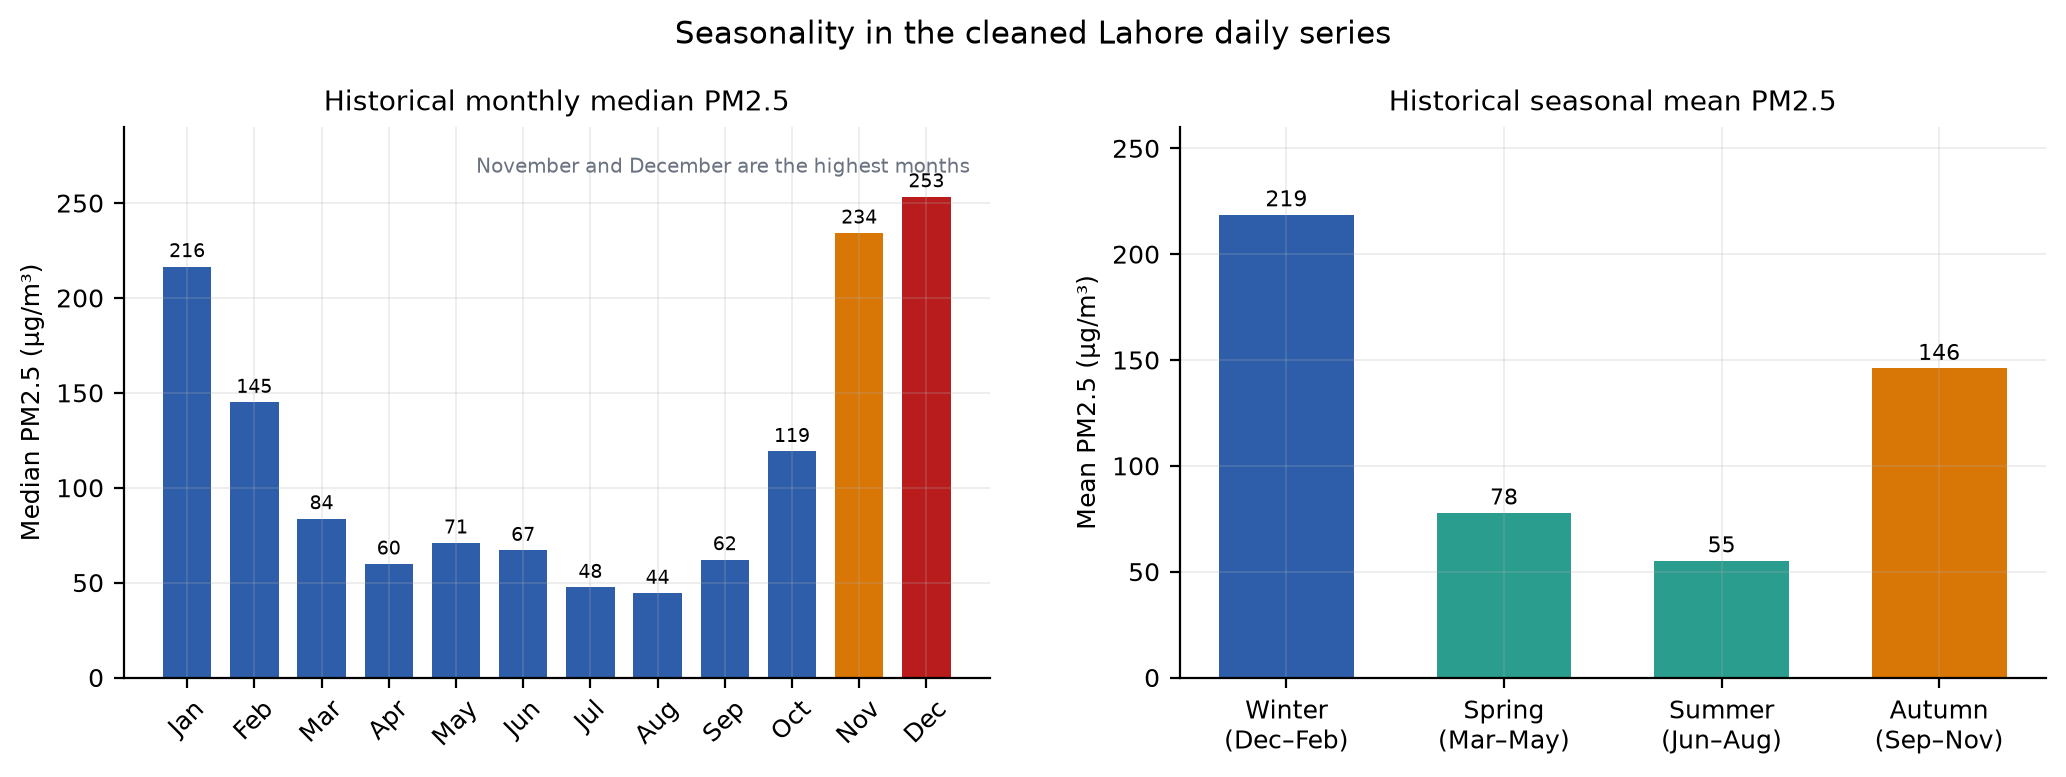
\includegraphics[width=\linewidth]{fig_seasonal.png}
  \caption{Historical monthly medians and seasonal means. November and December
  are the highest months; summer is much cleaner. These are descriptive
  statistics from one station, not a forecast.}
  \label{fig:d3-seasonal}
\end{figure}

\paragraph{Winter stagnation.} The app also reports a simple historical pattern.
A winter day (December--February) is labelled \emph{stagnant} when its mean wind
speed is in the winter lower quartile and it recorded at most 0.5 mm of rain. Of
407 winter days, 100 (24.6\%) meet the definition. Their mean PM$_{2.5}$ is
294.9 $\mu$g/m$^3$, versus 193.7 $\mu$g/m$^3$ on better-ventilated days, a
difference of +52.2\%. The winter wind quartile threshold is 5.2 km/h. This is a
descriptive proxy for stagnation, not a dispersion model, and it should not be
read as a causal estimate of the effect of wind.

\begin{table}[htbp]
\centering
\small
\begin{tabular}{@{}lr@{}}
\toprule
\textbf{Quantity} & \textbf{Value} \\
\midrule
Winter days (Dec--Feb) & 407 \\
Stagnant days & 100 (24.6\%) \\
Winter wind lower quartile & 5.2 km/h \\
Mean PM$_{2.5}$ on stagnant days & 294.9 $\mu$g/m$^3$ \\
Mean PM$_{2.5}$ on ventilated days & 193.7 $\mu$g/m$^3$ \\
Difference & +52.2\% \\
\bottomrule
\end{tabular}
\caption{Winter stagnation summary. The definition is descriptive and the
difference is associational.}
\label{tab:stagnation}
\end{table}

\paragraph{Seasonal means.} The seasonal means are 218.6 $\mu$g/m$^3$ in winter,
146.0 in autumn, 77.7 in spring, and 55.1 in summer. These values are the
context for the app's guidance: a November forecast that looks lower than today
can still be \emph{Very Unhealthy}, and a winter afternoon that is cleaner than
the morning can still be far above the WHO guideline. The app says this
explicitly rather than implying that timing solves the problem.

\subsection{The hourly profile}
\label{sec:d3-hourly}

The hourly card uses 36,820 valid hourly observations from the Lahore US
Diplomatic Post sensor, covering 2019-05-23 to 2025-02-18. The overall cleanest
three-hour window is 14:00--16:59, with a mean PM$_{2.5}$ of 85.2
$\mu$g/m$^3$; the worst hour is 22:00, with 138.4 $\mu$g/m$^3$. The afternoon
minimum holds in every season, but the winter version of the same window still
averages 155.4 $\mu$g/m$^3$, versus 41.2 in spring, 44.4 in summer, and 90.8 in
autumn. Timing helps; it does not make winter air safe.

\begin{table}[htbp]
\centering
\small
\begin{tabular}{@{}lr@{}}
\toprule
\textbf{Window or season} & \textbf{Mean PM$_{2.5}$} \\
\midrule
Cleanest overall window (14:00--16:59) & 85.2 $\mu$g/m$^3$ \\
Worst hour (22:00) & 138.4 $\mu$g/m$^3$ \\
Winter cleanest window (14:00--16:59) & 155.4 $\mu$g/m$^3$ \\
Spring cleanest window & 41.2 $\mu$g/m$^3$ \\
Summer cleanest window & 44.4 $\mu$g/m$^3$ \\
Autumn cleanest window & 90.8 $\mu$g/m$^3$ \\
\bottomrule
\end{tabular}
\caption{The hourly profile. The source is a single station and the values are
descriptive history, not a today-specific hourly forecast.}
\label{tab:hourly}
\end{table}

\begin{figure}[htbp]
  \centering
  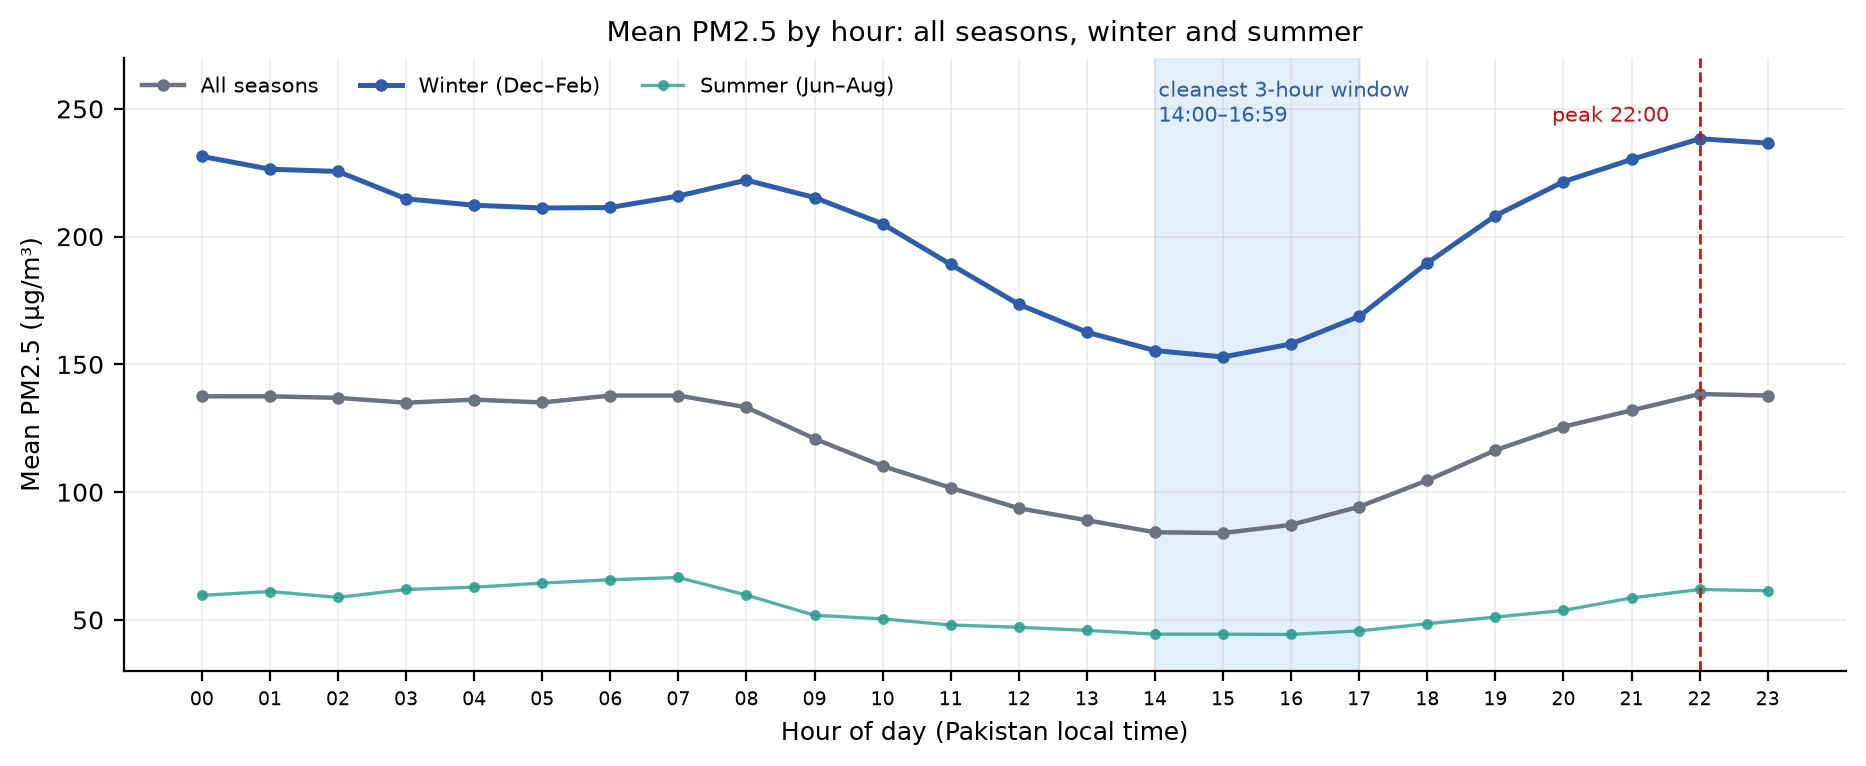
\includegraphics[width=\linewidth]{fig_hourly.png}
  \caption{Mean PM$_{2.5}$ by hour for all seasons, winter, and summer. The
  shaded window is the overall cleanest three hours; the dashed line marks the
  worst hour. Winter afternoons remain polluted.}
  \label{fig:d3-hourly}
\end{figure}

The card carries a caveat in the app: it is a descriptive station history in
Pakistan local time, not a today-specific forecast. The hourly source file is not
committed; if it is absent, the app omits the card and the rest of the pipeline
still runs.

\subsection{Persistence, guidance, and the honesty contract}
\label{sec:d3-honesty}

The app displays persistence on every forecast. Table~\ref{tab:persistence}
repeats the comparison that drives the report's framing. On the test split, the
regression's RMSE is 64.92 versus 64.82 for persistence, a difference of 0.10
$\mu$g/m$^3$ and a skill score of $-0.0016$. The classifier's macro-F1 is 0.4780
versus 0.5157 for persistence, even though the classifier's accuracy is slightly
higher (0.5856 versus 0.5676). The accuracy/macro-F1 split is the key: accuracy
is dominated by the common \emph{Unhealthy} class, while macro-F1 gives the rare
hazardous classes equal weight.

\begin{table}[htbp]
\centering
\small
\begin{tabular}{@{}lrrrr@{}}
\toprule
\textbf{Task and model} & \textbf{Validation} & \textbf{Test} &
\textbf{Persistence validation} & \textbf{Persistence test} \\
\midrule
Regression, HGB RMSE & 45.62 & 64.92 & 51.55 & 64.82 \\
Classification, HGB macro-F1 & 0.4941 & 0.4780 & 0.4766 & 0.5157 \\
\bottomrule
\end{tabular}
\caption{The frozen model versus persistence. The regression ties persistence on
test; the classifier loses on macro-F1. Ridge reached a lower test RMSE (62.10)
but was not the validation-selected model, so it is not used.}
\label{tab:persistence}
\end{table}

When the two category views disagree, the app shows a warning and says that the
implied category is the more defensible view because the classifier was weaker
than persistence on test. This is a deliberate design choice: hiding the
disagreement would make the interface look more confident than the evidence
supports.

\paragraph{Guidance.} The guidance text is keyed to the regression-implied
category and is cautious and non-medical. Table~\ref{tab:guidance} lists the
headlines. Every message carries a disclaimer that it is not a substitute for
official health advice. The app does not tell a user that it is safe to exercise;
it tells a user when to consider reducing exertion and when to avoid prolonged
outdoor activity.

\begin{table}[htbp]
\centering
\small
\begin{tabular}{@{}L{5.2cm}L{9.0cm}@{}}
\toprule
\textbf{Implied category} & \textbf{Headline} \\
\midrule
Good/Moderate & Air quality is relatively favourable. \\
Unhealthy for Sensitive & Sensitive groups should take care. \\
Unhealthy & Consider reducing outdoor exertion. \\
Very Unhealthy & Avoid prolonged outdoor activity. \\
Hazardous (301--400) & Avoid outdoor activity. \\
Hazardous (401--500) & Avoid outdoor activity. \\
\bottomrule
\end{tabular}
\caption{Cautious guidance by implied AQI category. The app adds a non-medical
disclaimer to every message.}
\label{tab:guidance}
\end{table}

\subsection{Tests and reproducibility}
\label{sec:d3-tests}

The application layer has 14 unit tests. They cover the EPA breakpoints and
category mapping, the feature schema and defaults, the interval bounds, the
local explanation, the guidance dictionary, the seasonal/stagnation patterns,
the monthly medians, and the hourly profile. The Streamlit AppTest adds a render
smoke test: no exceptions, four charts, and three expanders.

\begin{table}[htbp]
\centering
\small
\begin{tabular}{@{}L{4.4cm}L{10.0cm}@{}}
\toprule
\textbf{Test area} & \textbf{What is checked} \\
\midrule
AQI conversion & Breakpoints and category labels match the training labels \\
Feature contract & The app builds the expected columns, with the expected defaults \\
Intervals & Bounds contain the point forecast and respect the calibration factor \\
Explanation & Sensitivity returns the four perturbations in the expected shape \\
Guidance & Every category has a headline, detail, and disclaimer \\
Patterns & Stagnation, seasonal means, monthly medians, and hourly profile are present \\
App render & AppTest reports no exceptions, four charts, and three expanders \\
\bottomrule
\end{tabular}
\caption{Test coverage for the Deliverable 3 application layer.}
\label{tab:tests}
\end{table}

The reproducibility check is stronger than the test suite. Refitting the D3
pipelines from the committed script reproduces the Deliverable 2 metrics exactly:
regression validation/test RMSE 45.6243/64.9198, persistence 51.5457/64.8175;
classification validation/test macro-F1 0.4941/0.4780, persistence
0.4766/0.5157; interval coverage 80.3\%/77.0\%. The D2 code and report were not
edited. The D3 training script adds the two classifier settings that were needed
to match D2 exactly: balanced class weights and disabled early stopping. The
model itself is unchanged.

\section{Phase 6: Final Evaluation and Discussion}
\label{sec:phase6}

This section integrates the six phases, evaluates the application as a whole,
and states what the project can and cannot claim. The central finding is
negative but useful: the frozen model does not beat persistence, and the
application is designed to say so.

\subsection{Integrated results across phases}
\label{sec:integrated}

Table~\ref{tab:integrated} summarizes the delivered phases. The project moved
from a problem definition and a documented dataset, through a validation-selected
model and a bias analysis, to an application and an honest final evaluation.
The model scores did not change between Deliverable 2 and Deliverable 3.

\begin{table}[htbp]
\centering
\footnotesize
\begin{tabular}{@{}L{2.2cm}L{4.7cm}L{7.5cm}@{}}
\toprule
\textbf{Phase} & \textbf{Main output} & \textbf{Headline} \\
\midrule
Phase 1 & Problem definition and objectives &
1,506 valid days; only 9 Good days (0.6\%); 73.2\% Unhealthy or worse \\
Phase 2 & Data foundations and EDA &
2,113 daily rows, 63 columns, 2019-05-23 to 2025-03-04; one station \\
Phase 3 & Model development and selection &
HGB selected on validation: RMSE 45.62, macro-F1 0.4941 \\
Phase 4 & Evaluation and bias analysis &
Test RMSE 64.92 vs persistence 64.82; macro-F1 0.478 vs 0.516; severe-tail
errors are the largest \\
Phase 5 & Application and explainability &
Six inputs, two category views, 80\% interval, local/global explanations,
seasonal defaults, stagnation, hourly profile \\
Phase 6 & Final evaluation and discussion &
Ablation, backtest, limitations, reproducibility, and an honest verdict: the
app demonstrates the pipeline; it does not beat persistence \\
\bottomrule
\end{tabular}
\caption{Integrated results across the six phases.}
\label{tab:integrated}
\end{table}

The contribution is not a new accuracy record. It is an end-to-end, reproducible
system that makes a difficult result visible: a strong one-day persistence
baseline is hard to beat with the available features, and the remaining errors
are concentrated on the most severe pollution days, which are exactly the days
that matter most for public health.

\subsection{Ablation: do weather and calendar features help?}
\label{sec:ablation}

The ablation refits both tasks on three nested feature sets with the frozen
hyperparameters: history only (12 features), history plus calendar (29), and the
full set (46). Test metrics are reported but never used to choose a set. The
results are in Table~\ref{tab:ablation} and Figure~\ref{fig:d3-ablation}.

\begin{table}[htbp]
\centering
\footnotesize
\setlength{\tabcolsep}{4.5pt}
\begin{tabular}{@{}lrrrrr@{}}
\toprule
\textbf{Feature set} & \textbf{Feat.} &
\textbf{Reg. val} & \textbf{Reg. test} &
\textbf{Clf. val} & \textbf{Clf. test} \\
\midrule
History only & 12 & 52.18 & 63.88 & 0.4663 & 0.4715 \\
History + calendar & 29 & 49.97 & 65.16 & 0.4319 & 0.5155 \\
Full (adds weather) & 46 & \textbf{45.62} & \textbf{64.92} & \textbf{0.4941} & \textbf{0.4780} \\
\bottomrule
\end{tabular}
\caption{Nested feature-set ablation. Reg. columns are RMSE
($\mu$g/m$^3$); Clf. columns are macro-F1. Bold marks the validation-selected
full model. Test values are reported, not used for selection.}
\label{tab:ablation}
\end{table}

\begin{figure}[htbp]
  \centering
  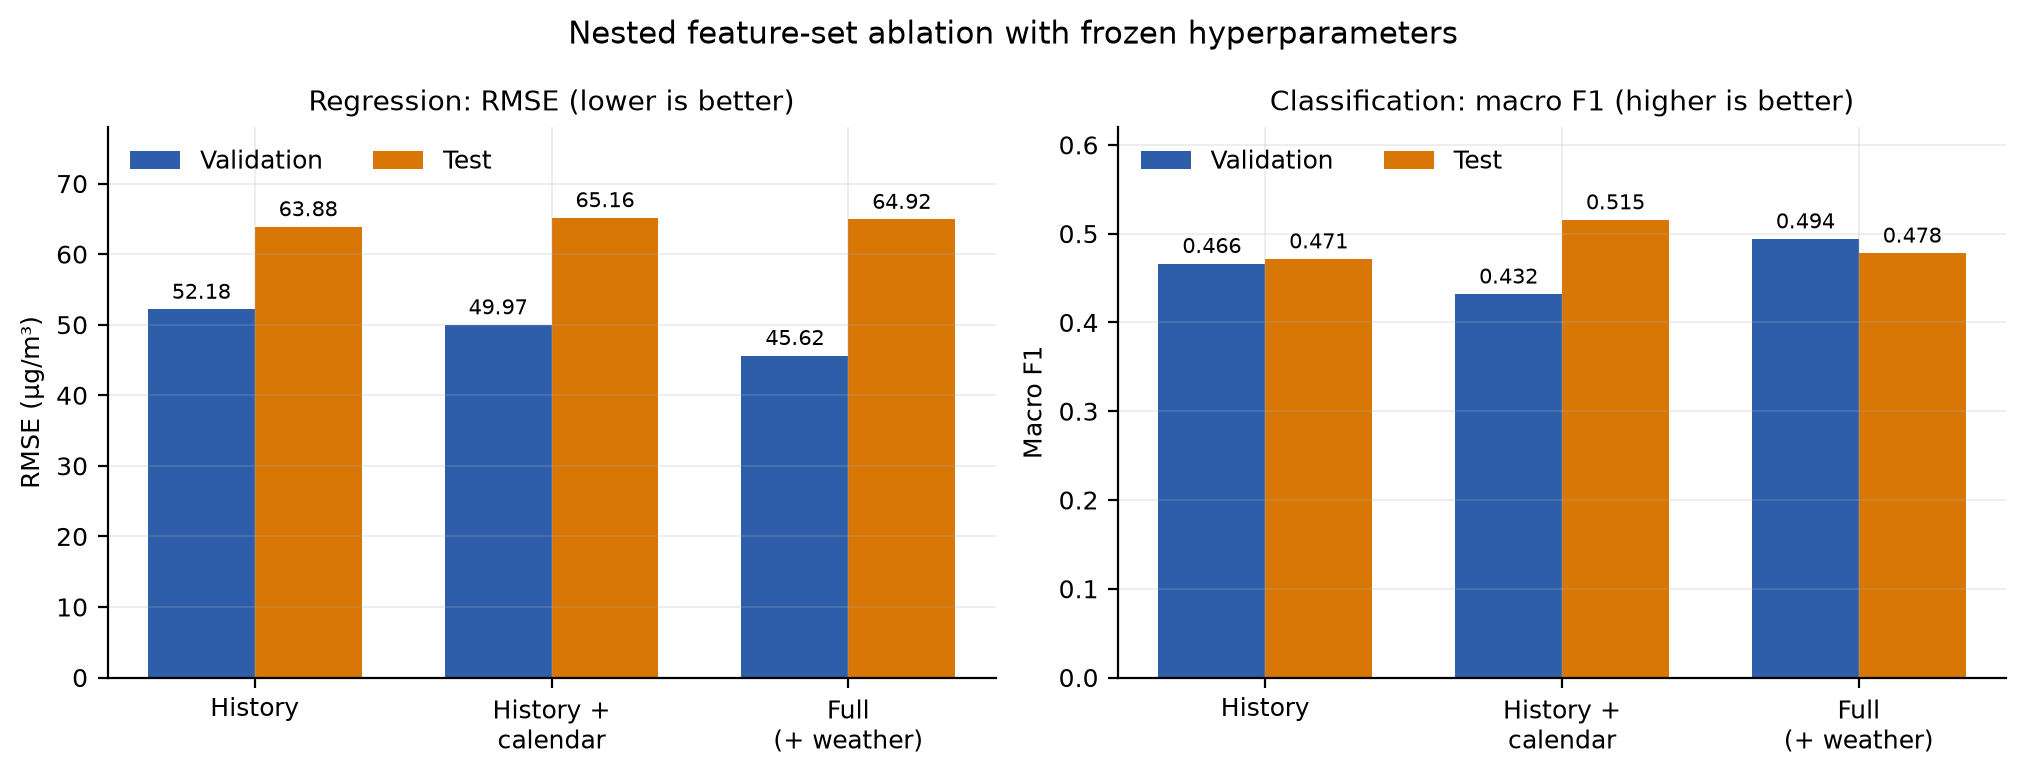
\includegraphics[width=\linewidth]{fig_ablation.png}
  \caption{Ablation results. The full model is best on validation for both tasks,
  but the test pattern is mixed: calendar features help classification and hurt
  regression, and the full model is not consistently best on test.}
  \label{fig:d3-ablation}
\end{figure}

The full model is best on validation for both tasks, which is why it is the
delivered model. The test pattern is mixed. Adding calendar features improves
classification test macro-F1 from 0.4715 to 0.5155 but lowers regression test
RMSE from 63.88 to 65.16. The full model then improves validation but gives back
some test performance. The honest conclusion is that there is no consistent
held-out gain from adding weather and calendar features on this dataset. The
ablation is descriptive, not a second model-selection step; switching to the
history-plus-calendar classifier after seeing test would violate the
validation-only rule.

\subsection{Backtest: 1 November 2024}
\label{sec:backtest}

A single backtest makes the application's limitations concrete. The feature date
is 1 November 2024, which is in the test split. Today's PM$_{2.5}$ is 156.6
$\mu$g/m$^3$. The app's six-input forecast is 159.23 $\mu$g/m$^3$, with an 80\%
interval of 101.7--209.7. The full-feature pipeline, using the actual history and
weather for that date, forecasts 188.23. The observed next-day PM$_{2.5}$ is
278.86. Persistence is 156.6. The actual value is outside the app's interval.

\begin{figure}[H]
  \centering
  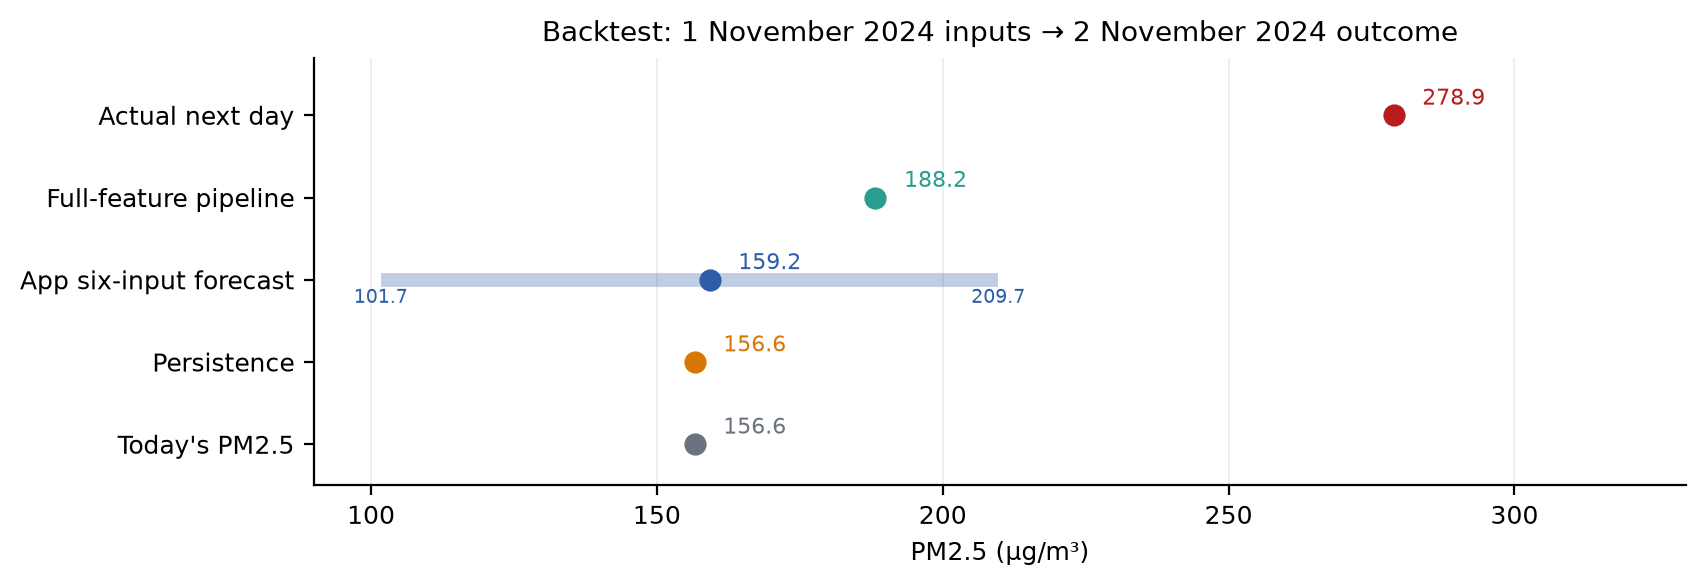
\includegraphics[width=0.96\linewidth]{fig_backtest.png}
  \caption{Backtest for 1 November 2024. The app forecast is close to
  persistence and far below the actual outcome; the full-feature model is
  closer but still under-predicts. This is the severe-tail failure that the bias
  analysis identified.}
  \label{fig:d3-backtest}
\end{figure}

\begin{table}[H]
\centering
\small
\begin{tabular}{@{}lr@{}}
\toprule
\textbf{Quantity} & \textbf{Value} \\
\midrule
Feature date & 1 November 2024 \\
Today's PM$_{2.5}$ & 156.6 $\mu$g/m$^3$ \\
App six-input forecast & 159.23 $\mu$g/m$^3$ \\
App 80\% interval & 101.7--209.7 $\mu$g/m$^3$ \\
Full-feature pipeline forecast & 188.23 $\mu$g/m$^3$ \\
Actual next-day PM$_{2.5}$ (2 November 2024) & 278.86 $\mu$g/m$^3$ \\
Persistence & 156.6 $\mu$g/m$^3$ \\
\bottomrule
\end{tabular}
\caption{Backtest for 1 November 2024. The app forecast and the full-feature
forecast both under-predict the severe day; the app's interval misses the
actual value.}
\label{tab:backtest}
\end{table}

The difference between 159.23 and 188.23 is informative. The app does not have
the actual previous days' PM$_{2.5}$ or the actual weather, so it assumes a
steady state and uses training medians for uncollected weather features. The
full-feature pipeline has the real inputs. Even with those inputs, it
under-predicts a severe day by about 91 $\mu$g/m$^3$. The app's lower forecast is
not evidence that the simpler interface is better; it is a consequence of
different information. The interval is wide, but not wide enough for this
outlier. With 77\% test coverage, some misses are expected; the important point
is that the miss is on a high-severity day, where the cost of under-prediction is
largest.

\subsection{What the app can and cannot claim}
\label{sec:claims}

Table~\ref{tab:claims} separates the defensible claims from the indefensible
ones. The app is a demonstration of an end-to-end explainable pipeline. It is not
an operational air-quality warning system.

\begin{table}[htbp]
\centering
\small
\begin{tabular}{@{}L{7.2cm}L{7.2cm}@{}}
\toprule
\textbf{The app can support} & \textbf{The app cannot support} \\
\midrule
A next-day PM$_{2.5}$ and AQI-category forecast from six inputs &
A claim that the forecast beats persistence on held-out data \\
A calibrated 80\% interval with reported validation and test coverage &
A guarantee that the interval contains the outcome \\
Local sensitivity and global permutation importance &
A causal claim about the effect of weather or policy \\
Seasonal context: monthly medians, stagnation, and the hourly profile &
A claim that winter afternoons are safe \\
A persistence comparison and a disagreement warning &
A claim that the classifier is reliable for rare hazardous classes \\
A reproducible artifact pipeline and 14 tests &
A live feed, a multi-day forecast, or a city-wide nowcast \\
Cautious, non-medical guidance &
Medical advice or a substitute for official advisories \\
\bottomrule
\end{tabular}
\caption{Defensible and indefensible claims for the Deliverable 3 application.}
\label{tab:claims}
\end{table}

\subsection{Limitations and ethics}
\label{sec:limitations-d3}

Table~\ref{tab:limitations-d3} consolidates the limitations from the model, the
data, and the application. The list is long because the project is deliberately
honest about what a single-station, six-input, one-day forecaster can do.

\begin{table}[htbp]
\centering
\footnotesize
\begin{tabular}{@{}L{3.8cm}L{5.7cm}L{5.5cm}@{}}
\toprule
\textbf{Limitation} & \textbf{Consequence} & \textbf{Mitigation or future work} \\
\midrule
One monitoring station & Results may not generalise to other neighbourhoods &
Add stations and a spatial validation design \\
Regression ties persistence; classifier loses & No evidence of an accuracy gain &
Report the baseline; treat the model as a demonstrator \\
Severe-tail under-prediction & The highest-risk days are the hardest &
Cost-sensitive training, quantile models, conformal intervals \\
Six inputs and many defaults & The forecast is illustrative, not live &
Ingest live weather and history; expose data provenance \\
Steady-state lags and rolling means & Rapid changes are under-represented &
Use the actual previous days' PM$_{2.5}$ \\
Classifier bias toward \emph{Unhealthy} & Category probabilities are overconfident &
Calibrate probabilities; use the implied category \\
80\% interval covers 77.0\% on test & Slight under-coverage &
Recalibrate on more data; add conformal prediction \\
Rare hazardous classes & Per-class metrics are noisy &
Collect more severe days; report support \\
Distribution shift & Validation-to-test reversals are possible &
Rolling-origin validation; monitor drift \\
No traffic data & Calendar features are proxies &
Integrate traffic and emissions data \\
Guidance is non-medical & Users may over-rely on the app &
Keep the disclaimer; link to official advisories \\
Single-station environmental justice & No demographic or neighbourhood fairness claim &
Add monitors and a population-aware evaluation \\
\bottomrule
\end{tabular}
\caption{Consolidated limitations and mitigations.}
\label{tab:limitations-d3}
\end{table}

\paragraph{Ethics.} The app processes no personal data and runs locally. If it
were deployed publicly, it would need authentication where appropriate, rate
limits, logging, a privacy review, and a clear separation between the
demonstration and official health advice. The guidance is intentionally
cautious: it tells users when to consider reducing exertion, not that a
particular activity is safe. The single-station limitation is also an equity
issue: a monitor at one location cannot represent the exposure of the whole
city, and the dataset contains no demographic attributes with which to test
fairness across groups.

\subsection{Reproducibility and repository guide}
\label{sec:repro-d3}

Table~\ref{tab:repro} lists the commands needed to rebuild the application and
the report from the committed source. All commands are run from the
\texttt{deliverable\_3} folder unless noted otherwise.

\begin{table}[H]
\centering
\footnotesize
\begin{tabular}{@{}L{3.2cm}L{7.4cm}L{4.0cm}@{}}
\toprule
\textbf{Step} & \textbf{Command} & \textbf{Expected output} \\
\midrule
Refit artifacts & \texttt{python -m src.train\_pipeline} &
Four joblib files and \texttt{metadata.json} \\
Run tests & \texttt{python -m unittest discover -s tests -t .} &
14 tests pass \\
Run ablation & \texttt{python -m src.ablation} &
\texttt{models/ablation.json} \\
Run app & \texttt{python -m streamlit run app/app.py} &
Local browser UI \\
Build figures & \texttt{python report/make\_figures.py} &
Report figures and \texttt{examples.json} \\
Build report & \texttt{tectonic report\_d3.tex} &
\texttt{report\_d3.pdf} \\
\bottomrule
\end{tabular}
\caption{Reproduction commands. The data files must be restored from the shared
Drive or regenerated from the data scripts before the refit. Append \texttt{-v}
to the test command for verbose output.}
\label{tab:repro}
\end{table}

The artifact policy is the same as in Deliverable 2: no fitted model binary and
no processed data file is committed. The \texttt{models/.gitignore} excludes the
joblib files, \texttt{metadata.json}, and \texttt{ablation.json}; the repository
root ignores the processed data. The refit is deterministic because the
hyperparameters and the random seed are fixed. The report figures are generated
from the persisted artifacts by \texttt{report/make\_figures.py}, so the report
and the app cannot silently diverge.

\paragraph{File map.} The D3 source is small enough to audit: \texttt{app/app.py}
is the interface; \texttt{src/inference.py} is the serving contract;
\texttt{src/train\_pipeline.py} refits the four pipelines and builds the
metadata; \texttt{src/ablation.py} runs the nested feature-set comparison;
\texttt{src/hourly.py} builds the hourly profile; \texttt{tests/test\_inference.py}
contains the 14 tests; \texttt{report/make\_figures.py} builds the report
figures; and \texttt{report/report\_d3.tex} is this report. The D1 and D2 reports
and code are unchanged.

\subsection{Conclusion and future work}
\label{sec:conclusion}

Deliverable 3 delivers a working, reproducible, explainable next-day air-quality
application for Lahore. The user enters six values; the app returns a PM$_{2.5}$
forecast, two category views, an 80\% interval, local and global explanations,
seasonal context, and a persistence comparison. The model is the frozen
Deliverable 2 model. It ties persistence on regression and loses to persistence
on classification macro-F1. The report does not hide that result, and the app
does not hide it either.

The most defensible contribution is the combination of a rigorous
validation-only modelling protocol, a calibrated uncertainty layer, an
explainable interface, a seasonal and hourly context, and a reproducibility
policy that regenerates every artifact from committed scripts. The project is
useful as a teaching and demonstration system, and as a foundation for a
stronger operational model.

Future work should proceed in the order that the evidence demands. First, ingest
live weather and PM$_{2.5}$ history so the inference layer does not rely on
steady-state assumptions. Second, add a second station and a rolling-origin
validation design to test whether the model generalises across place and time.
Third, improve the severe tail with cost-sensitive training, quantile or
conformal intervals, and a classifier that is calibrated rather than merely
arg-maxed. Fourth, replace the one-at-a-time sensitivity with a Shapley-value
decomposition if a more principled local explanation is needed. Finally, run a
small user study before making any public-health claim. Until then, the app
should remain a demonstration, and the official advisories should remain the
source of actionable guidance.


\appendix
% Appendices for the final SmogShield report.

\section{Viva questions and answers}
\label{app:viva}

\begin{description}[leftmargin=1.2em,style=nextline,itemsep=4pt]
  \item[What does the app predict?]
  It predicts tomorrow's PM$_{2.5}$ concentration and tomorrow's AQI category
  from six values for today: date, PM$_{2.5}$, AQI category, temperature,
  humidity, and wind speed. The forecast is always for the day after the
  selected feature date.

  \item[Why are there two AQI category views?]
  The classifier is a direct six-class model. The implied category converts the
  regression's predicted PM$_{2.5}$ through the same US-EPA breakpoints used to
  build the labels, so it is monotonic in the prediction. The classifier was
  weaker than persistence on test, so the app treats the implied category as the
  more defensible view and warns when the two disagree.

  \item[Does the model beat persistence?]
  No. On test, regression RMSE is 64.92 versus 64.82 for persistence, a
  0.10 $\mu$g/m$^3$ difference and a skill score of $-0.0016$. Classification
  macro-F1 is 0.4780 versus 0.5157. Ridge reached a lower test RMSE (62.10), but
  it was not the validation-selected model, so switching to it after seeing test
  would violate the validation-only rule.

  \item[Why keep a model that does not beat persistence?]
  The project is an end-to-end explainable system, not an accuracy record. The
  model was selected on validation, the test result is reported honestly, and
  the application demonstrates inference, uncertainty, explanations, and
  reproducibility. Persistence is a strong one-day baseline because PM$_{2.5}$ is
  highly autocorrelated; failing to beat it is an informative result.

  \item[What is HGB?]
  Histogram-based gradient boosting. It builds an ensemble of small decision
  trees sequentially, with each tree correcting the errors of the previous ones.
  The histogram step bins continuous features for speed. It handles non-linear
  relationships, interactions, and missing values, and it needs little
  preprocessing. The frozen settings were selected on validation in Deliverable
  2.

  \item[What is persistence?]
  Persistence assumes tomorrow will be the same as today: predicted value at
  $t+1$ equals the observed value at $t$. For classification, tomorrow's
  category equals today's. It is the simplest possible forecast and the baseline
  every model must beat.

  \item[Why macro-F1 instead of accuracy?]
  Accuracy is dominated by the common \emph{Unhealthy} class. Macro-F1 gives each
  class equal weight, so it exposes poor performance on the rare hazardous
  classes. The HGB classifier has slightly higher test accuracy than persistence
  but lower macro-F1; reporting only accuracy would obscure the rare-class
  weakness.

  \item[What does the 80\% interval mean?]
  It is a central interval for the next-day PM$_{2.5}$ observation, built from
  quantile HGB models at the 10th and 90th percentiles and calibrated on
  validation. Validation coverage is 80.3\%; test coverage is 77.0\%. The test
  split is used only to report coverage, never to choose the calibration factor.

  \item[Why is the interval so wide?]
  The model is uncertain, especially on severe days. The default November
  example forecasts 189.74 $\mu$g/m$^3$ with an interval of 133.8--294.1. The
  width is an honest statement about the evidence, not a bug. The backtest on
  1 November 2024 shows that the actual value can fall outside the interval when
  the day is an extreme outlier.

  \item[Why only six inputs?]
  Usability. The remaining features use training medians or modes, and the
  PM$_{2.5}$ lags and rolling windows are held at today's value. The app calls
  itself an illustrative single-day forecaster for this reason. A production
  version would ingest live weather and a multi-day PM$_{2.5}$ history.

  \item[What changed after Deliverable 2?]
  The model and its reported scores are unchanged; the D3 refit reproduces D2
  exactly. What is new is the application layer: inference, the Streamlit app,
  prediction intervals, explanations, the ablation, the hourly profile, the
  seasonal defaults, and the tests. The D2 code and report were not edited.

  \item[What is the biggest limitation?]
  The single monitoring station and the severe-tail under-prediction. The model
  is weakest on the highest-pollution days, which are exactly the days that
  matter most for public health. A second station, live inputs, and a
  cost-sensitive or conformal approach are the next steps.
\end{description}

\section{Glossary}
\label{app:glossary}

\begin{longtable}{@{}L{3.6cm}L{11.0cm}@{}}
\toprule
\textbf{Term} & \textbf{Meaning in this project} \\
\midrule
\endhead
\bottomrule
\endfoot
PM$_{2.5}$ & Fine particulate matter with diameter at most 2.5 $\mu$m, measured
in $\mu$g/m$^3$. The regression target. \\
AQI & Air Quality Index, a 0--500 scale computed from PM$_{2.5}$ using the US-EPA
2012 breakpoints. \\
HGB & Histogram-based gradient boosting; an ensemble of small trees trained
sequentially to correct errors. \\
Regression & Predicting a continuous number, here tomorrow's PM$_{2.5}$. \\
Classification & Predicting a discrete class, here tomorrow's AQI category. \\
Persistence & The baseline ``tomorrow equals today.'' \\
RMSE & Root mean squared error; same units as the target and sensitive to large
errors. \\
MAE & Mean absolute error; average absolute miss, in the target's units. \\
$R^2$ & Fraction of variance explained; 1 is perfect and 0 is no better than the
mean. \\
Macro-F1 & The unweighted mean of per-class F1 scores; treats each class equally
and exposes rare-class performance. \\
Weighted-F1 & F1 weighted by class support; dominated by the common classes. \\
Precision and recall & Of the predicted positives, how many are correct; of the
true positives, how many were found. \\
Confusion matrix & A table of predicted versus true classes. \\
Prediction interval & A range for a future observation, here the central 80\%. \\
Quantile regression & Training a model to predict a conditional percentile rather
than the mean. \\
Coverage & The fraction of true values that fall inside the interval. \\
Calibration & Adjusting interval width so empirical coverage matches the nominal
level. \\
Permutation importance & Global importance: the increase in error when a feature
is shuffled. \\
Sensitivity & Local importance: the change in the forecast when one input is
perturbed. \\
Ablation & Removing feature groups to test whether they improve performance. \\
Data leakage & Information from validation or test contaminating training;
prevented here by the seven-day purge and train-only preprocessing. \\
Class imbalance & Some categories are much rarer than others; handled with
balanced class weights and macro-F1. \\
Piecewise constant & A tree model's prediction stays flat inside a leaf, so a
small input change may have no effect. \\
Steady state & The app's assumption that today's PM$_{2.5}$ has been stable for
the past week when it fills lags and rolling windows. \\
\end{longtable}

\section{File map and build notes}
\label{app:files}

Table~\ref{tab:filemap} lists the Deliverable 3 files a reviewer is most likely
to open. The full repository map also includes the Deliverable 1 data scripts and
the Deliverable 2 modelling code, which are unchanged.

\begin{table}[htbp]
\centering
\footnotesize
\begin{tabular}{@{}L{5.4cm}L{9.2cm}@{}}
\toprule
\textbf{File} & \textbf{Role} \\
\midrule
\texttt{app/app.py} & Streamlit interface: six inputs, forecast cards, interval,
guidance, charts, expanders \\
\texttt{src/inference.py} & Loads the four pipelines and metadata; assembles the
feature row; predicts PM$_{2.5}$, category, interval, explanation, and guidance \\
\texttt{src/train\_pipeline.py} & Refits the frozen pipelines; writes the joblib
artifacts and \texttt{metadata.json} \\
\texttt{src/ablation.py} & Runs the nested history/calendar/weather ablation \\
\texttt{src/hourly.py} & Builds the hour-of-day and seasonal PM$_{2.5}$ profile \\
\texttt{tests/test\_inference.py} & Fourteen unit tests for the inference and app
contract \\
\texttt{report/make\_figures.py} & Generates the report figures and the worked
examples from the frozen artifacts \\
\texttt{report/report\_d3.tex} & This report's master LaTeX file \\
\texttt{report/phase34\_final.tex} & Deliverable 2 Phase 3--4 body, reused with
adjusted table paths \\
\texttt{report/phase56\_final.tex} & New Deliverable 3 Phase 5--6 chapters \\
\texttt{report/appendix\_final.tex} & Viva questions, glossary, and file map \\
\texttt{README.md} & Install, run, artifact, and submission notes \\
\texttt{STUDY\_REPORT.md} & Plain-language technical study report \\
\texttt{requirements.txt} & Python dependencies for the application layer \\
\bottomrule
\end{tabular}
\caption{Deliverable 3 file map.}
\label{tab:filemap}
\end{table}

\paragraph{Build notes.} The report is compiled from the
\texttt{deliverable\_3/report} directory with Tectonic:
\begin{verbatim}
tectonic report_d3.tex
\end{verbatim}
The \texttt{report/make\_figures.py} script must be run first if the figures or
\texttt{examples.json} are missing. The model artifacts must be present for the
script to compute the worked examples; run \texttt{python -m src.train\_pipeline}
from \texttt{deliverable\_3} first. The report's numerical tables are taken from
the frozen D2 metrics and the D3 metadata, ablation, and worked-example files.


\begin{thebibliography}{9}

\bibitem{majeed2024lahore}
R. Majeed, M. S. Anjum, M. Imad-ud-din, S. Malik, M. N. Anwar, B. Anwar, and M. F. Khokhar,
``Solving the mysteries of Lahore smog: the fifth season in the country,''
\emph{Frontiers in Sustainable Cities}, vol.~5, art.~1314426, 2024.
doi:10.3389/frsc.2023.1314426.

\bibitem{who2024ambient}
World Health Organization,
``Ambient (outdoor) air pollution,'' fact sheet, 24 October 2024.
[Online]. Available: \url{https://www.who.int/news-room/fact-sheets/detail/ambient-(outdoor)-air-quality-and-health}

\bibitem{epa_pm_basics}
U.S. Environmental Protection Agency,
``Particulate Matter (PM) Basics.''
[Online]. Available: \url{https://www.epa.gov/pm-pollution/particulate-matter-pm-basics}

\bibitem{epa_aqi_tad}
U.S. Environmental Protection Agency,
``Technical Assistance Document for the Reporting of Daily Air Quality -- the Air Quality Index (AQI),'' EPA-454/B-18-007, September 2018.
[Online]. Available: \url{https://www.airnow.gov/sites/default/files/2020-05/aqi-technical-assistance-document-sept2018.pdf}

\bibitem{waqas2024lahore}
H. M. S. Waqas, T. Naz, K. Shahid, A. Yaqoob, and M. B. Ahmad,
``Time series forecasting of air quality index in Lahore: a machine learning perspective with Facebook Prophet model,''
\emph{International Journal of Scientific Research in Science and Technology}, vol.~11, no.~5, pp.~219--226, 2024.
doi:10.32628/IJSRST2411598.

\bibitem{scikit}
F. Pedregosa, G. Varoquaux, A. Gramfort, V. Michel, B. Thirion, O. Grisel, M. Blondel, P. Prettenhofer, R. Weiss, V. Dubourg, J. Vanderplas, A. Passos, D. Cournapeau, M. Brucher, M. Perrot, and E. Duchesnay,
``Scikit-learn: Machine learning in Python,''
\emph{Journal of Machine Learning Research}, vol.~12, pp.~2825--2830, 2011.

\bibitem{hgb}
J. H. Friedman,
``Greedy function approximation: a gradient boosting machine,''
\emph{Annals of Statistics}, vol.~29, no.~5, pp.~1189--1232, 2001.

\bibitem{streamlit}
Streamlit,
``Streamlit documentation,'' 2026.
[Online]. Available: \url{https://docs.streamlit.io/}

\end{thebibliography}

\end{document}
